\chapter{The best academic Computer Science Depts: A ranking case study}
\label{sec:13}

\abstract*{ In this case study, we are solving with our \Digraph resources a ranking decision problem based on published data from the \emph{Times Higher Education} (THE) \emph{World University Rankings} 2016 by \emph{Computer Science} (CS) subject. Several hundred academic CS Departments, from all over the world, were ranked that year following an overall numerical score based on the weighted average of five performance criteria: \emph{Teaching} (the learning environment, $30\%$), \emph{Research} (volume, income and reputation, $30\%$), \emph{Citations} (research influence, $27.5\%$), \emph{International outlook} (staff, students, and research, $7.5\%$), and \emph{Industry income} (innovation, $5\%$). To illustrate our \Digraph programming resources, we shall first have a look into the THE ranking data with short Python scripts. In a second section, we shall relax the commensurability hypothesis of the ranking criteria and show how to similarly rank with multiple incommensurable performance criteria of solely ordinal significance. A third Section is finally devoted to introduce quality measures for qualifying ranking results.}

\abstract{ In this case study, we are solving with our \Digraph resources a ranking decision problem based on published data from the \emph{Times Higher Education} (THE) \emph{World University Rankings} 2016 by \emph{Computer Science} (CS) subject. Several hundred academic CS Departments, from all over the world, were ranked that year following an overall numerical score based on the weighted average of five performance criteria: \emph{Teaching} (the learning environment, $30\%$), \emph{Research} (volume, income and reputation, $30\%$), \emph{Citations} (research influence, $27.5\%$), \emph{International outlook} (staff, students, and research, $7.5\%$), and \emph{Industry income} (innovation, $5\%$). To illustrate our \Digraph programming resources, we shall first have a look into the THE multiple criteria ranking data with short Python scripts. In a second section, we shall relax the commensurability hypothesis of the ranking criteria and show how to similarly rank with multiple incommensurable performance criteria of solely ordinal significance. A third section is finally devoted to introduce quality measures for qualifying ranking results.
}

\section{The THE performance tableau}
\label{sec:13.1}

For this decision making case study, we use an extract of the published \THE (THE) World University rankings 2016 by Computer Science (CS) subject, concerning the 75 first-ranked academic Institutions\footnote{\href{https://www.timeshighereducation.com/world-university-rankings/2017/subject-ranking/computer-science}{THE World University Rankings 2016 by Computer Science subject}}. The multiple criteria performance tableau data, collected from the THE web pages, is stored in a file named \texttt{the-cs-2016.py} of \texttt{PerformanceTableau} format \footnote{The performance tableau \texttt{the-cs-2016.py} is available in the \texttt{examples} directory of the \Digraph resources \citep{BIS-2021}.}.\index{THE University rankings 2016 by CS subject} 
\begin{lstlisting}[caption={Performance tableau of the },label=list:13.1]
>>> from perfTabs import PerformanceTableau
>>> cspt = PerformanceTableau('the_cs_2016')
>>> cspt
  *------- PerformanceTableau instance description ------*
   Instance class     : PerformanceTableau
   Instance name      : the-cs-2016
   Actions            : 75
   Objectives         : 5
   Criteria           : 5
   NaN proportion (%) : 0.0
   Attributes         : ['name','description','actions',
                           'objectives','criteria',
			   'weightPreorder','NA','evaluation']
\end{lstlisting}

Potential decision alternatives, in our case here, are the 75 THE best-ranked CS Departments in 2016, all of them located at world renowned Institutions, like California Institute of Technology, Swiss Federal Institute of Technology Zurich, Technical University München, University of Oxford or the National University of Singapore (see List.~\vref{list:13.2} below). 

Instead of using prefigured \Digraph \texttt{show...()} methods, readily available for inspecting \texttt{PerformanceTableau} instances, Listing~\vref{list:13.2} below illstrates how to write small Python scripts for printing out its content.   
\begin{lstlisting}[caption={Printing the CS Departments},label=list:13.2,basicstyle=\ttfamily\scriptsize]
>>> for x in cspt.actions:
...     print('%s:\t%s (%s)' %\
...        (x,cspt.actions[x]['name'],cspt.actions[x]['comment']) )
  albt:	University of Alberta (CA)
  anu:	Australian National University (AU)
  ariz:	Arizona State University (US)
  bju:	Beijing University (CN)
  bro:	Brown University (US)
  calt:	California Institute of Technology (US)
  cbu:	Columbia University (US)
  chku:	Chinese University of Hong Kong (HK)
  cihk:	City University of Hong Kong (HK)
  cir:	University of California at Irvine (US)
  cmel:	Carnegie Mellon University (US)
  cou:	Cornell University (US)
  csb:	University of California at Santa Barbara (US)
  csd:	University Of California at San Diego (US)
  dut:	Delft University of Technology (NL)
  eind:	Eindhoven University of Technology (NL)
  ens:	Superior Normal School at Paris (FR)
  epfl:	Swiss Federal Institute of Technology Lausanne (CH)
  epfr:	Polytechnic school of Paris (FR)
  ethz:	Swiss Federal Institute of Technology Zurich (CH)
  frei:	University of Freiburg (DE)
  git:	Georgia Institute of Technology (US)
  glas:	University of Glasgow (UK)
  hels:	University of Helsinki (FI)
  hkpu:	Hong Kong Polytechnic University (CN)
  hkst:	Hong Kong University of Science and Technology (HK)
  hku:	Hong Kong University (HK)
  humb:	Berlin Humboldt University (DE)
  icl:	Imperial College London (UK)
  indis:Indian Institute of Science (IN)
  itmo:	ITMO University (RU)
  kcl:	King's College London (UK)
  kist:	Korea Adv. Institute of Science and Technology (KR)
  kit:	Karlsruhe Institute of Technology (DE)
  kth:	KTH Royal Institute of Technology (SE)
  kuj:	Kyoto University (JP)
  kul:	Catholic University Leuven (BE)
  lms:	Lomonosov Moscow State University (RU)
  man:	University of Manchester (UK)
  mcp:	University of Maryland College Park (US)
  mel:	University of Melbourne (AU)
  mil:	Polytechnic University of Milan (IT)
  mit:	Massachusetts Institute of Technology (US)
  naji:	Nanjing University (CN)
  ntu:	Nanyang Technological University of Singapore (SG)
  ntw:	National Taiwan University (TW)
  nyu:	New York University (US)
  oxf:	University of Oxford (UK)
  pud:	Purdue University (US)
  qut:	Queensland University of Technology (AU)
  rcu:	Rice University (US)
  rwth:	RWTH Aachen University (DE)
  shJi:	Shanghai Jiao Tong University (CN)
  sing:	National University of Singapore (SG)
  sou:	University of Southhampton (UK)
  stut:	University of Stuttgart (DE)
  tech:	Technion - Israel Institute of Technology (IL)
  tlavu:Tel Aviv University (IR)
  tsu:	Tsinghua University (CN)
  tub:	Technical University of Berlin (DE)
  tud:	Technical University of Darmstadt (DE)
  tum:	Technical University of Muenchen (DE)
  ucl:	University College London (UK)
  ued:	University of Edinburgh (UK)
  uiu:	University of Illinois at Urbana-Champagne (US)
  unlu:	University of Luxembourg (LU)
  unsw:	University of New South Wales (AU)
  unt:	University of Toronto (CA)
  uta:	University of Texas at Austin (US)
  utj:	University of Tokyo (JP)
  utw:	University of Twente (NL)
  uwa:	University of Waterloo (CA)
  wash:	University of Washington (US)
  wtu:	Vienna University of Technology (AUS)
  zhej:	Zhejiang University (CN)
\end{lstlisting}

The THE authors base their 2016 ranking on five decision objectives \citep{THE-2016}.
\begin{lstlisting}[caption={The THE ranking objectives},label=list:13.3,basicstyle=\ttfamily\scriptsize]
>>> for obj in cspt.objectives:
...     print('%s: %s (%.1f%%),\n\t%s' %\
...                (obj,cspt.objectives[obj]['name'],\
...                 cspt.objectives[obj]['weight'],
...                 cspt.objectives[obj]['comment'])\
...           ) 
 Teaching: Best learning environment (30.0%)
   Reputation survey; Staff-to-student ration;
   Doctorate-to-student ratio;
   Doctorate-to-academic-staff ratio;
   Institutional income.
 Research: Highest volume and reputation (30.0%)
   Reputation survey;
   Research income;
   Research productivity.
 Citations: Highest research influence (27.5%)
   Impact.
 International outlook: Most international staff,
                        students and research (7.5%)
   Proportions of international students;
   Proportions of international staff;
   International collaborations.
 Industry income: Best knowledge transfer (5.0%)
   Volume.
\end{lstlisting}

With a cumulated importance of $87\%$ (see above), \emph{Teaching}, \emph{Research} and \emph{Citations} represent clearly the major ranking objectives. \emph{International outlook} and \emph{Industry income} are considered of minor importance ($12.5\%$).

THE authors do, unfortunately, not publish the detail of their performance assessments for grading CS Depts with respect to each one of performance criteria per ranking objective.  \footnote{THE gives some insight on the subject and significance of the actual ranking criteria used for grading along each ranking objective on her website \citep{THE-2016}}. The THE 2016 ranking publication reveals solely a compound assessment on a single performance criteria per ranking objective. The five retained performance criteria may be printed out as follows.
\begin{lstlisting}
>>> for g in cspt.criteria:
...     print('%s:\t%s, %s (%.1f%%)' %\
...       (g,cspt.criteria[g]['name'],cspt.criteria[g]['comment'],\
...        cspt.criteria[g]['weight']) )  
  gtch:	Teaching, The learning environment (30.0%)
  gres:	Research, Volume, income and reputation (30.0%)
  gcit:	Citations, Research influence (27.5%)
  gint:	International outlook, In staff, students and research (7.5%)
  gind:	Industry income, knowledge transfer (5.0%)
\end{lstlisting}

The largest part ($87.5\%$) of criteria significance is, hence canonically, allocated to the major ranking criteria: \emph{Teaching} ($30\%$), \emph{Research} ($30\%$) and \emph{Citations} ($27.5\%$). The small remaining part ($12.5\%$) goes to \emph{International outlook} ($7.5\%$) and \emph{Industry income} ($5\%$).

In order to render commensurable these performance criteria, the THE authors replace, per criterion, the actual performance grade obtained by each University with the corresponding \emph{quantile} observed in the cumulative distribution of the performance grades obtained by all the surveyed institutions \citep{THE-2016}. The THE ranking is eventually determined by an \emph{overall score} per University which corresponds to the weighted average of these five criteria quantiles, as illustrated in Listing~\vref{list:13.4} below.     
\begin{lstlisting}[caption={Computing the THE overall scores},label=list:13.4]
>>> theScores = []
>>> for x in cspt.actions:
...     xscore = Decimal('0')
...     for g in cspt.criteria:
...         xscore += cspt.evaluation[g][x] *\
...          (cspt.criteria[g]['weight']/Decimal('100'))
...	   theScores.append((xscore,x))
\end{lstlisting}

In Listing~\vref{list:13.5} (Lines 15-16), we may thus notice that, in the 2016 edition of the THE World University rankings by CS subject, the Swiss Federal Institute of Technology Zürich is first-ranked with an overall score of $92.9$; followed by the California Institute of Technology (overall score: $92.4$) \footnote{The author's own Computer Science Dept at the University of Luxembourg was ranked on position 63 with an overall score of $58.0$.}.
\begin{lstlisting}[caption={Printing the ranked performance table},label=list:13.5,basicstyle=\ttfamily\scriptsize]
>>> theScores.sort(reverse = True)
>>> print('##  Univ \tgtch  gres  gcit  gint  gind  overall')
>>> print('-------------------------------------------------') 
>>> i = 1
>>> for it in theScores:
...     x = it[1]
...     xScore = it[0]
...     print('%2d: %s' % (i,x), end=' \t')
...     for g in cspt.criteria:
...         print('%.1f ' % (cspt.evaluation[g][x]),end=' ')
...	    print(' %.1f' % xScore)
...         i += 1   
    ##  Univ 	gtch  gres  gcit  gint  gind  overall
    -------------------------------------------------
     1: ethz 	89.2  97.3  97.1  93.6  64.1   92.9
     2: calt 	91.5  96.0  99.8  59.1  85.9   92.4
     3: oxf 	94.0  92.0  98.8  93.6  44.3   92.2
     4: mit 	87.3  95.4  99.4  73.9  87.5   92.1
     5: git 	87.2  99.7  91.3  63.0  79.5   89.9
     6: cmel 	88.1  92.3  99.4  58.9  71.1   89.4
     7: icl 	90.1  87.5  95.1  94.3  49.9   89.0
     8: epfl 	86.3  91.6  94.8  97.2  42.7   88.9
     9: tum 	87.6  95.1  87.9  52.9  95.1   87.7
    10: sing 	89.9  91.3  83.0  95.3  50.6   86.9
    11: cou 	81.6  94.1  99.7  55.7  45.7   86.6
    12: ucl 	85.5  90.3  87.6  94.7  42.4   86.1
    13: wash 	84.4  88.7  99.3  57.4  41.2   85.6
    14: hkst 	74.3  92.0  96.2  84.4  55.8   85.5
    15: ntu 	76.6  87.7  90.4  92.9  86.9   85.5
    16: ued 	85.7  85.3  89.7  95.0  38.8   85.0
    17: unt 	79.9  84.4  99.6  77.6  38.4   84.4
    18: uiu 	85.0  83.1  99.2  51.4  42.2   83.7
    19: mcp 	79.7  89.3  94.6  29.8  51.7   81.5
    20: cbu 	81.2  78.5  94.7  66.9  45.7   81.3
    21: tsu 	88.1  90.2  76.7  27.1  85.9   80.9
    22: csd 	75.2  81.6  99.8  39.7  59.8   80.5
    23: uwa 	75.3  82.6  91.3  72.9  41.5   80.0
    24: nyu 	71.1  77.4  99.4  78.0  39.8   79.7
    25: uta 	72.6  85.3  99.6  31.6  49.7   79.6
    26: kit 	73.8  85.5  84.4  41.3  76.8   77.9
    27: bju 	83.0  85.3  70.1  30.7  99.4   77.0
    28: csb 	65.6  70.9  94.8  72.9  74.9   76.2
    29: rwth 	77.8  85.0  70.8  43.7  89.4   76.1
    30: hku 	77.0  73.0  77.0  96.8  39.5   75.4
    31: pud 	76.9  84.8  70.8  58.1  56.7   75.2
    32: kist 	79.4  88.2  64.2  31.6  92.8   74.9
    33: kcl 	45.5  94.6  86.3  95.1  38.3   74.8
    34: chku 	64.1  69.3  94.7  75.6  49.9   74.2
    35: epfr 	81.7  60.6  78.1  85.3  62.9   73.7
    36: dut 	64.1  78.3  76.3  69.8  90.1   73.4
    37: tub 	66.2  82.4  71.0  55.4  99.9   73.3
    38: utj 	92.0  91.7  48.7  25.8  49.6   72.9
    39: cir 	68.8  64.6  93.0  65.1  40.4   72.5
    40: ntw 	81.5  79.8  66.6  25.5  67.6   72.0
    41: anu 	47.2  73.0  92.2  90.0  48.1   70.6
    42: rcu 	64.1  53.8  99.4  63.7  46.1   69.8
    43: mel 	56.1  70.2  83.7  83.3  50.4   69.7
    44: lms 	81.5  68.1  61.0  31.1  87.8   68.4
    45: ens 	71.8  40.9  98.7  69.6  43.5   68.3
    46: wtu 	61.8  73.5  73.7  51.9  62.2   67.9
    47: tech 	54.9  71.0  85.1  51.7  40.1   67.1
    48: bro 	58.5  54.9  96.8  52.3  38.6   66.5
    49: man 	63.5  71.9  62.9  84.1  42.1   66.3
    50: zhej 	73.5  70.4  60.7  22.6  75.7   65.3
    51: frei 	54.2  51.6  89.5  49.7  99.9   65.1
    52: unsw 	60.2  58.2  70.5  87.0  44.3   63.6
    53: kuj 	75.4  72.8  49.5  28.3  51.4   62.8
    54: sou 	48.2  60.7  75.5  87.4  43.2   62.1
    55: shJi 	66.9  68.3  62.4  22.8  38.5   61.4
    56: itmo 	58.0  32.0  98.7  39.2  68.7   60.5
    57: kul 	35.2  55.8  92.0  46.0  88.3   60.5
    58: glas 	35.2  52.5  91.2  85.8  39.2   59.8
    59: utw 	38.2  52.8  87.0  69.0  60.0   59.4
    60: stut 	54.2  60.6  61.1  36.3  97.8   58.9
    61: naji 	51.4  76.9  48.8  39.7  74.4   58.6
    62: tud 	46.6  53.6  75.9  53.7  66.5   58.3
    63: unlu 	35.2  44.2  87.4  99.7  54.1   58.0
    64: qut 	45.5  42.6  82.8  75.2  63.0   58.0
    65: hkpu 	46.8  36.5  91.4  73.2  41.5   57.7
    66: albt 	39.2  53.3  69.9  91.9  75.4   57.6
    67: mil 	46.4  64.3  69.2  44.1  38.5   57.5
    68: hels 	48.8  49.6  80.4  50.6  39.5   57.4
    69: cihk 	42.4  44.9  80.1  76.2  67.9   57.3
    70: tlavu 	34.1  57.2  89.0  45.3  38.6   57.2
    71: indis 	56.9  76.1  49.3  20.1  41.5   57.0
    72: ariz 	28.4  61.8  84.3  59.3  42.0   56.8
    73: kth 	44.8  42.0  83.6  71.6  39.2   56.4
    74: humb 	48.4  31.3  94.7  41.5  45.5   55.3
    75: eind 	32.4  48.4  81.5  72.2  45.8   54.4
\end{lstlisting}

It is important to notice that a ranking by weighted average scores requires \emph{commensurable ranking criteria} of precise decimal significance and on wich precise decimal performance grades are given. It is very unlikely that the THE 2016 performance assessments verify indeed these conditions. Here we show how to relax these methodological requirements --precise commensurable criteria and decimal grades-- by following instead a bipolar-valued epistemic logic based ranking methodology (see Chap.~\ref{sec:8}).

\section{Ranking with multiple criteria of ordinal significance}
\label{sec:13.2}

Let us, first, have a critical look in Figure~\vref{fig:13.1} at the THE performance criteria.
\begin{lstlisting}
>>> cspt.showHTMLCriteria(Sorted=False)
\end{lstlisting}
\begin{figure}[ht]
%\sidecaption
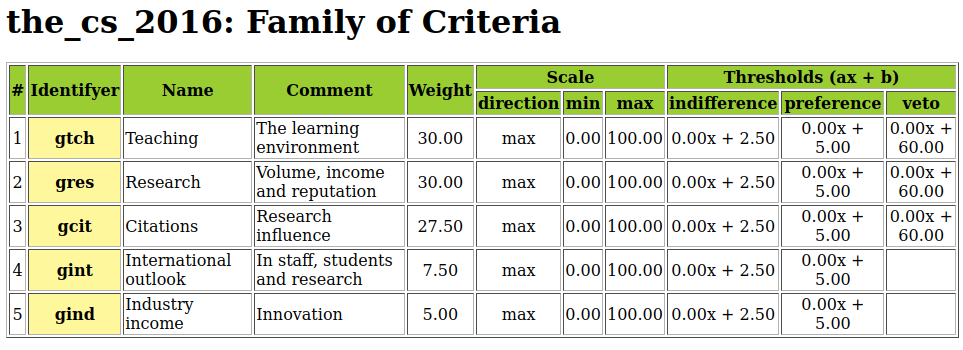
\includegraphics[width=\hsize]{Figures/13-1-the_cs_2016Criteria.png}
\caption{The THE ranking criteria}
\label{fig:13.1}       % Give a unique label
\end{figure}

Considering a very likely imprecision of the performance grading procedure, followed by some potential violation of uniform distributed quantile classes, we assume here that a performance quantile difference of up to $2.5\%$ is \emph{insignificant}, whereas a difference of $5\%$ and more warrants a \emph{clearly better}, resp. \emph{clearly less good} performance. With quantiles $94\%$, resp. $87.3\%$, Oxford's CS teaching environment, for instance, is thus clearly better evaluated than that of the MIT (see List.~\vref{list:13.5} Lines 27-28). We shall furthermore assume that a \emph{considerable} performance quantile difference of $60\%$, observed on the three major ranking criteria: \emph{Teaching}, \emph{Research} and \emph{Citations}, will trigger the polarisation of pairwise outranking, respectively outranked situations \citep{BIS-2013}.

The effect these performance discrimination thresholds induce on the outranking modelling can be inspected with the \texttt{showCriteria()} method\index{showCriteria@\texttt{showCriteria()}}.
\begin{lstlisting}[caption={Inspecting the performance discrimination thresholds},label=list:13.6]
>>> cspt.showCriteria()
  *----  criteria -----*
    gtch 'Teaching'
      Scale = (Decimal('0.00'), Decimal('100.00'))
      Weight = 0.300 
      Threshold ind : 2.50 + 0.00x ;   percentile:  8.07
      Threshold pref : 5.00 + 0.00x ;  percentile: 15.75
      Threshold veto : 60.00 + 0.00x ; percentile: 99.75
    gres 'Research'
      Scale = (Decimal('0.00'), Decimal('100.00'))
      Weight = 0.300 
      Threshold ind : 2.50 + 0.00x ;   percentile:  7.86
      Threshold pref : 5.00 + 0.00x ;  percentile: 16.14
      Threshold veto : 60.00 + 0.00x ; percentile: 99.21
    gcit 'Citations'
      Scale = (Decimal('0.00'), Decimal('100.00'))
      Weight = 0.275 
      Threshold ind : 2.50 + 0.00x ;   percentile:  11.82
      Threshold pref : 5.00 + 0.00x ;  percentile:  22.99
      Threshold veto : 60.00 + 0.00x ; percentile: 100.00
    gint 'International outlook'
      Scale = (Decimal('0.00'), Decimal('100.00'))
      Weight = 0.075 
      Threshold ind : 2.50 + 0.00x ;  percentile:  6.45
      Threshold pref : 5.00 + 0.00x ; percentile: 11.75
    gind 'Industry income'
      Scale = (Decimal('0.00'), Decimal('100.00'))
      Weight = 0.050 
      Threshold ind : 2.50 + 0.00x ;  percentile: 11.82
      Threshold pref : 5.00 + 0.00x ; percentile: 21.51
\end{lstlisting}

Between $6\%$ and $12\%$ of the observed quantile differences are, hence, considered to be \emph{insignificant}. Similarly, between $77\%$ and $88\%$ are considered to be \emph{significant}. Less than $1\%$ correspond to \emph{considerable} quantile differences on both the \emph{Teaching} and \emph{Research} criteria; actually triggering an epistemic polarisation effect \citep{BIS-2013}.

Beside the likely imprecise performance discrimination, the \emph{precise decimal significance weights}, as allocated by the THE authors to the five ranking criteria are, as well, quite \emph{questionable}. Criteria significance weights may carry sometimes hidden strategies for rendering the performance evaluations commensurable in view of a numerical computation of the overall ranking scores. The eventual ranking result is, the case given, as much depending on the precise values of the given criteria significance weights as, vice versa, the given precise significance weights are depending on the subjectively expected and accepted ranking results \footnote{In a social choice context, this potential double bind between voting profiles and election result, corresponds to voting manipulation strategies.}. We will therefore drop these precise decimal weights and, instead, only require a corresponding criteria significance preorder: \texttt{gtch} $=$ \texttt{gres} $>$ \texttt{gcit} $>$ \texttt{gint} $>$ \texttt{gind}. \emph{Teaching environment} and \emph{Research volume and reputation} are equally considered most significant, followed by \emph{Research influence}. Then comes \emph{International outlook in staff, students and research} and, least significant finally, \emph{Industry income and innovation}.

Both these working hypotheses: --performance discrimitation thresholds and --solely ordinal criteria significance, give us way to a ranking methodology based on \emph{robust pairwise outranking} situations (see Chap.~\ref{sec:19} and \citep{BIS-2004b}).
\begin{definition}[Robust outranking situations with ordinal criteria significance weights]\label{def:13.1}
\begin{itemize}[topsep=1pt]
\item We say that CS Dept $x$ \emph{robustly outranks} CS Dept $y$ when $x$ positively outranks $y$ with \textbf{all} significance weight vectors that are compatible with the significance preorder: \texttt{gtch} $=$ \texttt{gres} $>$ \texttt{gcit} $>$ \texttt{gint} $>$ \texttt{gind};
\item We say that CS Dept $x$ is \emph{robustly outranked} by CS Dept $y$ when $x$ is positively outranked by $y$ with \textbf{all} significance weight vectors that are compatible with the significance preorder: \texttt{gtch} $=$ \texttt{gres} $>$ \texttt{gcit} $>$ \texttt{gint} $>$ \texttt{gind};
\item Otherwise, CS Depts $x$ and $y$ are considered to be \emph{incomparable}.
\end{itemize}
\end{definition}

A corresponding digraph constructor is provided by the \texttt{RobustOutranking\-Digraph} class\index{RobustOutrankingDigraph@\texttt{RobustOutrankingDigraph} class}.
\begin{lstlisting}[caption={Computing the robust outranking digraph},label=list:13.7]
>>> from outrankingDigraphs import RobustOutrankingDigraph	     
>>> rdg = RobustOutrankingDigraph(cspt)
>>> rdg
  *------- Object instance description ------*
   Instance class       : RobustOutrankingDigraph
   Instance name        : robust_the_cs_2016
   Actions              : 75
   Criteria             : 5
   Size                 : 2993
   Determinateness (%)  : 78.16
   Valuation domain     : [-1.00;1.00]
>>> rdg.computeIncomparabilityDegree(Comments=True)
  Incomparability degree (%) of digraph <robust_the_cs_2016>:
   links x<->y y: 2775, incomparable: 102, comparable: 2673
   (incomparable/links) =  0.037
>>> rdg.computeTransitivityDegree(Comments=True)
  Transitivity degree of digraph <robust_the_cs_2016>:
   triples x>y>z: 405150, closed: 218489, open: 186661
   (closed/triples) =  0.539
>>> rdg.computeSymmetryDegree(Comments=True)
  Symmetry degree (%) of digraph <robust_the_cs_2016>:
   arcs x>y: 2673, symmetric: 320, asymmetric: 2353
   (symmetric/arcs) =  0.12
\end{lstlisting}

In the resulting digraph instance \texttt{rdg} (see Line 9 in Listing~\vref{list:13.7}), we observe $2993$ such robust pairwise outranking situations validated with a mean significance of $78\%$ (Line 10). Unfortunately, in the case here, they do not deliver any complete linear ranking. The robust outranking digraph \texttt{rdg} contains 102 incomparability situations ($3.7\%$, Line 15); nearly half of its transitive closure is missing ($46.1\%$, Line 19) and $12\%$ of the positive outranking situations correspond in fact to symmetric indifference situations (Line 23).

Worse even, the digraph \texttt{rdg} admits a really high number of outranking circuits.\index{showChordlessCircuits@\texttt{showChordlessCircuits()}}
\begin{lstlisting}[caption={Inspecting outranking circuits},label=list:13.8]
>>> rdg.computeChordlessCircuits()
>>> rdg.showChordlessCircuits()
 *---- Chordless circuits ----*
  145 circuits.
  1:  ['albt','unlu','ariz','hels'], cred. : 0.300
  2:  ['albt','tlavu','hels'], cred. : 0.150
  3:  ['anu', 'man', 'itmo'], cred. : 0.250
  4:  ['anu', 'zhej', 'rcu'], cred. : 0.250
    ...
    ...
  82:  ['csb','epfr','rwth'], cred. : 0.250
  83:  ['csb','epfr','pud','nyu'], cred. : 0.250
  84:  ['csd','kcl','kist'], cred. : 0.250
    ...
    ...
  142:  ['kul','qut','mil'], cred. : 0.250
  143:  ['lms','rcu','tech'], cred. : 0.300
  144:  ['mil','stut','qut'], cred. : 0.300
  145:  ['mil','stut','tud'], cred. : 0.300
\end{lstlisting}

Among the 145 detected robust outranking circuits reported in Listing \vref{list:13.8}, we notice, for instance, two outranking circuits of length 4 (see circuits 1 and 83).

Let us inspect below the bipolar-valued robust outranking characteristics of the first circuit.
\begin{lstlisting}[caption={Showing the relation table with stability denotation},label=list:13.9]
>>> rdg.showRelationTable(actionsSubset=\
...         ['albt','unlu','ariz','hels'],\
...         Sorted=False) 
  * ---- Relation Table -----
   r/(stab)|  'albt' 'unlu' 'ariz' 'hels'   
      -----|-----------------------------
    'albt' |  +1.00  +0.30  +0.00  +0.00  
           |   (+4)   (+2)   (-1)   (-1)  
    'unlu' |  +0.00  +1.00  +0.40  +0.00  
           |   (+0)   (+4)   (+2)   (-1)  
    'ariz' |  +0.00  -0.12  +1.00  +0.40  
           |   (+1)   (-2)   (+4)   (+2)  
    'hels' |  +0.45  +0.00  -0.03  +1.00  
           |   (+2)   (+1)   (-2)   (+4)  
   Valuation domain: [-1.0; 1.0]
   Stability denotation semantics:
   +4|-4 : unanimous outranking | outranked situation;
   +2|-2 : outranking | outranked situation validated
      with all potential significance weights that are
      compatible with the given significance preorder;
   +1|-1 : validated outranking | outranked situation
      with the given significance weights;
     0   : indeterminate relational situation.
\end{lstlisting}

In Listing~\vref{list:13.9}, we notice that the robust outranking circuit \texttt{[albt,} \texttt{unlu,} \texttt{ariz,} \texttt{hels]}  will reappear with all potential criteria significance weight vectors that are compatible with given preorder: \texttt{gtch} $=$ \texttt{gres} $>$ \texttt{gcit} $>$ \texttt{gint} $>$ \texttt{gind}. Notice also the ($\pm 1$) marked outranking situations, like the one between \texttt{albt} and \texttt{ariz}. The statement that ``\emph{Arizona State University strictly  outranks University of Alberta}'' is in fact valid with the precise THE criteria signifiance weights, but not with all potential significance weights vectors that are compatible with the given significance preorder. All these ($\pm 1$)  marked outranking situations become hence \emph{doubtful} ($r(x \succsim y) = 0.00$) and the corresponding CS Depts, like University of Alberta and Arizona State University, become \emph{incomparable} in a robust outranking sense.  

Showing many incomparabilities and indifferences; not being transitive and containing many robust outranking circuits; all these relational characteristics, make that no ranking algorithm, applied to digraph \texttt{rdg}, does exist that would produce a \emph{unique} optimal linear ranking result. Methodologically, we are only left with ranking heuristics. In Chapter~\ref{sec:8} on ranking with multiple criteria we have now seen several potential heuristic ranking rules that can be used for ranking with an outranking digraph; yet, they may deliver potentially more or less diverging results. Considering the order of digraph \texttt{rdg} (75) and the largely unequal THE criteria significance weights, we rather opt, in this tutorial, for the \NetFlows ranking rule \footnote{The reader might try other ranking rules, like the \Copeland or \Kohler rules. Mind that the latter ranking-by-choosing rule is more complex (see Chap.~\ref{sec:8}).}. Its complexity in $O(n^2)$ is indeed quite tractable and, by avoiding potential \emph{tyranny of short majority} effects, the \NetFlows rule may specifically take the ranking criteria significance weights into a more fairly balanced account.

The \NetFlows ranking result of the CS Depts can be directly computed with the \texttt{computeNetFlowsRanking()} method\index{computeNetFlowsRanking@\texttt{computeNetFlowsRanking()}}. 
\begin{lstlisting}[caption={Computing a robust \NetFlows ranking},label=list:13.10]
>>> nfRanking = rdg.computeNetFlowsRanking()
>>> nfRanking
  ['ethz','calt','mit', 'oxf',  'cmel','git', 'epfl',
   'icl', 'cou', 'tum', 'wash', 'sing','hkst','ucl',
   'uiu', 'unt', 'ued', 'ntu',  'mcp', 'csd', 'cbu',
   'uta', 'tsu', 'nyu', 'uwa',  'csb', 'kit', 'utj',
   'bju', 'kcl', 'chku','kist', 'rwth','pud', 'epfr',
   'hku', 'rcu', 'cir', 'dut',  'ens', 'ntw', 'anu',
   'tub', 'mel', 'lms', 'bro',  'frei','wtu', 'tech',
   'itmo','zhej','man', 'kuj',  'kul', 'unsw','glas',
   'utw', 'unlu','naji','sou',  'hkpu','qut', 'humb',
   'shJi','stut','tud', 'tlavu','cihk','albt','indis',
   'ariz','kth', 'hels','eind', 'mil']
\end{lstlisting}

We actually obtain in Listing~\vref{list:13.10} a very similar ranking result as the one obtained with the THE average scores. The same group of seven Depts: \texttt{ethz}, \texttt{calt}, \texttt{mit}, \texttt{oxf}, \texttt{cmel}, \texttt{git} and \texttt{epfl}, is top-ranked. And a same group of Depts: \texttt{tlavu}, \texttt{cihk}, \texttt{indis}, \texttt{ariz}, \texttt{kth}, \texttt{hels}, \texttt{eind}, and \texttt{mil} appears at the end of the list.

We can print out the difference between the overall scores based THE ranking and the \NetFlows ranking above with the following short Python script, where we make use of an ordered Python dictionary with net-flow scores, stored in the \texttt{rdg.netFlowsRankingDict} attribute by the previous computation.
\begin{lstlisting}[caption={Comparing the robust \NetFlows ranking with the THE ranking},label=list:13.11,basicstyle=\ttfamily\scriptsize]
>>> # rdg.netFlowsRankingDict: ordered dictionary with net flow
>>> # scores stored in rdg by the computeNetFlowsRanking() method
>>> # theScores = [(xScore_1,x_1), (xScore_2,x_2),... ]
>>> # is sorted in decreasing order of xscores_i
>>> print(\
...  ' NetFlows ranking   gtch  gres  gcit  gint  gind   THE ranking')
>>> for i in range(75):
...     x = nfRanking[i]
...     xScore = rdg.netFlowsRankingDict[x]['netFlow']
...     thexScore,thex = theScores[i]
...     print('%2d: %s (%.2f) ' % (i+1,x,xScore), end=' \t')
...     for g in rdg.criteria:
...         print('%.1f ' % (t.evaluation[g][x]),end=' ')
...     print(' %s (%.2f)' % (thex,thexScore) )  
  NetFlows ranking   gtch  gres  gcit  gint  gind   THE ranking
   1: ethz (116.95)  89.2  97.3  97.1  93.6  64.1   ethz (92.88)
   2: calt (116.15)  91.5  96.0  99.8  59.1  85.9   calt (92.42)
   3: mit (112.72)   87.3  95.4  99.4  73.9  87.5   oxf (92.20)
   4: oxf (112.00)   94.0  92.0  98.8  93.6  44.3   mit (92.06)
   5: cmel (101.60)  88.1  92.3  99.4  58.9  71.1   git (89.88)
   6: git (93.40)    87.2  99.7  91.3  63.0  79.5   cmel (89.43)
   7: epfl (90.88)   86.3  91.6  94.8  97.2  42.7   icl (89.00)
   8: icl (90.62)    90.1  87.5  95.1  94.3  49.9   epfl (88.86)
   9: cou (84.60)    81.6  94.1  99.7  55.7  45.7   tum (87.70)
  10: tum (80.42)    87.6  95.1  87.9  52.9  95.1   sing (86.86)
  11: wash (76.28)   84.4  88.7  99.3  57.4  41.2   cou (86.59)
  12: sing (73.05)   89.9  91.3  83.0  95.3  50.6   ucl (86.05)
  13: hkst (71.05)   74.3  92.0  96.2  84.4  55.8   wash (85.60)
  14: ucl (66.78)    85.5  90.3  87.6  94.7  42.4   hkst (85.47)
  15: uiu (64.80)    85.0  83.1  99.2  51.4  42.2   ntu (85.46)
  16: unt (62.65)    79.9  84.4  99.6  77.6  38.4   ued (85.03)
  17: ued (58.67)    85.7  85.3  89.7  95.0  38.8   unt (84.42)
  18: ntu (57.88)    76.6  87.7  90.4  92.9  86.9   uiu (83.67)
  19: mcp (54.08)    79.7  89.3  94.6  29.8  51.7   mcp (81.53)
  20: csd (46.62)    75.2  81.6  99.8  39.7  59.8   cbu (81.25)
  21: cbu (44.27)    81.2  78.5  94.7  66.9  45.7   tsu (80.91)
  22: uta (43.27)    72.6  85.3  99.6  31.6  49.7   csd (80.45)
  23: tsu (42.42)    88.1  90.2  76.7  27.1  85.9   uwa (80.02)
  24: nyu (35.30)    71.1  77.4  99.4  78.0  39.8   nyu (79.72)
  25: uwa (28.88)    75.3  82.6  91.3  72.9  41.5   uta (79.61)
  26: csb (18.18)    65.6  70.9  94.8  72.9  74.9   kit (77.94)
  27: kit (16.32)    73.8  85.5  84.4  41.3  76.8   bju (77.04)
  28: utj (15.95)    92.0  91.7  48.7  25.8  49.6   csb (76.23)
  29: bju (15.45)    83.0  85.3  70.1  30.7  99.4   rwth (76.06)
  30: kcl (11.95)    45.5  94.6  86.3  95.1  38.3   hku (75.41)
  31: chku (9.43)    64.1  69.3  94.7  75.6  49.9   pud (75.17)
  32: kist (7.30)    79.4  88.2  64.2  31.6  92.8   kist (74.94)
  33: rwth (5.00)    77.8  85.0  70.8  43.7  89.4   kcl (74.81)
  34: pud (2.40)     76.9  84.8  70.8  58.1  56.7   chku (74.23)
  35: epfr (-1.70)   81.7  60.6  78.1  85.3  62.9   epfr (73.71)
  36: hku (-3.83)    77.0  73.0  77.0  96.8  39.5   dut (73.44)
  37: rcu (-6.38)    64.1  53.8  99.4  63.7  46.1   tub (73.25)
  38: cir (-8.20)    68.8  64.6  93.0  65.1  40.4   utj (72.92)
  39: dut (-8.85)    64.1  78.3  76.3  69.8  90.1   cir (72.50)
  40: ens (-8.97)    71.8  40.9  98.7  69.6  43.5   ntw (72.00)
  41: ntw (-11.15)   81.5  79.8  66.6  25.5  67.6   anu (70.57)
  42: anu (-11.50)   47.2  73.0  92.2  90.0  48.1   rcu (69.79)
  43: tub (-12.20)   66.2  82.4  71.0  55.4  99.9   mel (69.67)
  44: mel (-23.98)   56.1  70.2  83.7  83.3  50.4   lms (68.38)
  45: lms (-25.43)   81.5  68.1  61.0  31.1  87.8   ens (68.35)
  46: bro (-27.18)   58.5  54.9  96.8  52.3  38.6   wtu (67.86)
  47: frei (-34.42)  54.2  51.6  89.5  49.7  99.9   tech (67.06)
  48: wtu (-35.05)   61.8  73.5  73.7  51.9  62.2   bro (66.49)
  49: tech (-37.95)  54.9  71.0  85.1  51.7  40.1   man (66.33)
  50: itmo (-38.50)  58.0  32.0  98.7  39.2  68.7   zhej (65.34)
  51: zhej (-43.70)  73.5  70.4  60.7  22.6  75.7   frei (65.08)
  52: man (-44.83)   63.5  71.9  62.9  84.1  42.1   unsw (63.65)
  53: kuj (-47.40)   75.4  72.8  49.5  28.3  51.4   kuj (62.77)
  54: kul (-49.98)   35.2  55.8  92.0  46.0  88.3   sou (62.15)
  55: unsw (-54.88)  60.2  58.2  70.5  87.0  44.3   shJi (61.35)
  56: glas (-56.98)  35.2  52.5  91.2  85.8  39.2   itmo (60.52)
  57: utw (-59.27)   38.2  52.8  87.0  69.0  60.0   kul (60.47)
  58: unlu (-60.08)  35.2  44.2  87.4  99.7  54.1   glas (59.78)
  59: naji (-60.52)  51.4  76.9  48.8  39.7  74.4   utw (59.40)
  60: sou (-60.83)   48.2  60.7  75.5  87.4  43.2   stut (58.85)
  61: hkpu (-62.05)  46.8  36.5  91.4  73.2  41.5   naji (58.61)
  62: qut (-66.17)   45.5  42.6  82.8  75.2  63.0   tud (58.28)
  63: humb (-68.10)  48.4  31.3  94.7  41.5  45.5   unlu (58.04)
  64: shJi (-69.72)  66.9  68.3  62.4  22.8  38.5   qut (57.99)
  65: stut (-69.90)  54.2  60.6  61.1  36.3  97.8   hkpu (57.69)
  66: tud (-70.83)   46.6  53.6  75.9  53.7  66.5   albt (57.63)
  67: tlavu (-71.50) 34.1  57.2  89.0  45.3  38.6   mil (57.47)
  68: cihk (-72.20)  42.4  44.9  80.1  76.2  67.9   hels (57.40)
  69: albt (-72.33)  39.2  53.3  69.9  91.9  75.4   cihk (57.33)
  70: indis (-72.53) 56.9  76.1  49.3  20.1  41.5   tlavu (57.19)
  71: ariz (-75.10)  28.4  61.8  84.3  59.3  42.0   indis (57.04)
  72: kth (-77.10)   44.8  42.0  83.6  71.6  39.2   ariz (56.79)
  73: hels (-79.55)  48.8  49.6  80.4  50.6  39.5   kth (56.36)
  74: eind (-82.85)  32.4  48.4  81.5  72.2  45.8   humb (55.34)
  75: mil (-83.67)   46.4  64.3  69.2  44.1  38.5   eind (54.36)
\end{lstlisting}

The first inversion we observe in Listing~\vref{list:13.11} (Lines 18-19) concerns Oxford University and the MIT, switching positions 3 and 4. Most inversions are similarly short and concern only switching very close positions in either way. There are some slightly more important inversions concerning, for instance, the Hong Kong University CS Dept, ranked into position 30 in the THE ranking and here in the position 36 (Line 51). The opposite situation may also happen; the Berlin Humboldt University CS Dept, occupying the 74th position in the THE ranking, advances in the robust \NetFlows ranking to position 63 (Line 78).

In our bipolar-valued epistemic framework, the \NetFlows score of any CS Dept $x$ corresponds to the criteria significance support for the logical statement ``$x$ \emph{is first-ranked}''. Formally 
\begin{equation}\label{eq:13.1}
  r(x \; \text{is first-ranked}) \; = \; \sum_{y \neq x} r\big((x \succsim y) \,+\, (y \not\succsim x)\big) \;=\; \sum_{y \neq x} \big(r(x \succsim y) - r(y \succsim x)\big).
\end{equation}

Using the robust outranking characteristics of digraph \texttt{rdg}, we can thus explicitly compute, for instance, ETH Zürich's \NetFlows score, denoted \texttt{nfx} below.
\begin{lstlisting}
>>> x = 'ethz'
>>> nfx = Decimal('0')
>>> for y in rdg.actions:
...     if x != y:
...         nfx += (rdg.relation[x][y]\
...                - rdg.relation[y][x])  
>>> print(x, nfx)
  ethz 116.950
\end{lstlisting}

In Listing~\vref{list:13.11} (Line 16), one may now verify that ETH Zürich obtains indeed the highest \NetFlows score $116.95$, and gives, hence the \emph{most credible} first-ranked CS Dept of the 75 potential candidates.

Yet, how may we now convince the reader, that the outranking based ranking result here appears more objective and trustworthy, than the classic value theory based THE ranking by average quantile scores?  

\section{How to judge the quality of a ranking result?}
\label{sec:13.3}

In a multiple criteria based ranking problem, inspecting pairwise marginal performance differences may give objectivity to global preferential statements. That a CS Dept $x$ convincingly outranks Dept $y$ can conveniently be checked with the \texttt{showPairwiseOutrankings()} method.\index{showPairwiseOutrankings@\texttt{showPairwiseOutrankings()}}. The ETH Zürich CS Dept is, for instance, first ranked before Caltech's Dept in both previous rankings. Lest us check the preferential reasons.
\begin{lstlisting}[caption={Comparing pairwise criteria performances},label=list:13.11,basicstyle=\ttfamily\scriptsize]
>>> rdg.showPairwiseOutrankings('ethz','calt')
  *------------  pairwise comparisons ----*
  Valuation in range: -100.00 to +100.00
  Comparing actions : ('ethz', 'calt')
  crit.    wght.  g(ethz)  g(calt) diff  | ind  pref     r()  | 
  --------------------------------------   -------------------
  'gcit'   27.50   97.10   99.80   -2.70 | 2.50  5.00   +0.00 | 
  'gind'    5.00   64.10   85.90  -21.80 | 2.50  5.00   -5.00 | 
  'gint'    7.50   93.60   59.10  +34.50 | 2.50  5.00   +7.50 | 
  'gres'   30.00   97.30   96.00   +1.30 | 2.50  5.00  +30.00 | 
  'gtch'   30.00   89.20   91.50   -2.30 | 2.50  5.00  +30.00 |
                                                     ------
                                         r(x >= y):  +62.50
  crit.    wght.  g(calt)  g(ethz) diff  | ind   pref    r()  |
  ---------------------------------------   -----------------
  'gcit'   27.50   99.80   97.10   +2.70 | 2.50  5.00  +27.50 | 
  'gind'    5.00   85.90   64.10  +21.80 | 2.50  5.00   +5.00 | 
  'gint'    7.50   59.10   93.60  -34.50 | 2.50  5.00   -7.50 | 
  'gres'   30.00   96.00   97.30   -1.30 | 2.50  5.00  +30.00 | 
  'gtch'   30.00   91.50   89.20   +2.30 | 2.50  5.00  +30.00 |
                                                      -------
                                            r(y >= x): +85.00
\end{lstlisting}

A significant positive performance difference ($+34.50$), concerning the \emph{International outlook} criterion (of $7,5\%$ significance), is observed in Listing~\vref{list:13.11} in favour of the ETH Zürich Dept (Line 9 above). Similarly, a significant positive performance difference ($+21.80$), concerning the \emph{Industry income} criterion (of $5\%$ significance), is observed, this time, in favour of the Caltech Dept (Line 17). The former, larger positive, performance difference, observed on a more significant criterion, gives so far a first convincing argument of $12.5\%$ significance for putting ETH Zürich first, before Caltech. Yet, the slightly positive performance difference ($+2.70$, Line 16) between Caltech and ETH Zürich on the \emph{Citations} criterion (of $27.5\%$ significance) confirms an ``\emph{at least as well performing as}'' situation in favour of the Caltech Dept.

The inverse negative performance difference ($-2.70$, Line 7), however, is neither \emph{significant} ($< -5.00$), nor \emph{insignificant} ($> -2.50$), and does hence neither confirm nor infirm a ``\emph{not at least as well performing as}'' situation in disfavour of ETH Zürich. We observe here a convincing argument of $27.5\%$ significance for ranking Caltech first, before ETH Zürich.

Notice finally, that, on the \emph{Teaching} and \emph{Research} criteria of total significance $60\%$, both Depts do, with performance differences $(< \mid 2.50 \mid)$, perform one as well as the other. As these two major performance criteria together necessarily admid always the highest significance with the imposed significance weight preorder: \texttt{gtch} $=$ \texttt{gres} $>$ \texttt{gcit} $>$ \texttt{gint} $>$ \texttt{gind}, both outranking situations get in fact globally confirmed at stability level $+2$ (see Chap.~\ref{sec:19}).

We may well illustrate all such \emph{stable outranking} situations with a browser view of the corresponding robust relation map ordering the CS Depts again with the same \NetFlows ranking rule.
\begin{lstlisting}
>>> rdg.showHTMLRelationMap(\
...            tableTitle='Robust Outranking Map',
...            rankingRule='NetFlows')
\end{lstlisting}
\begin{figure}[ht]
%\sidecaption
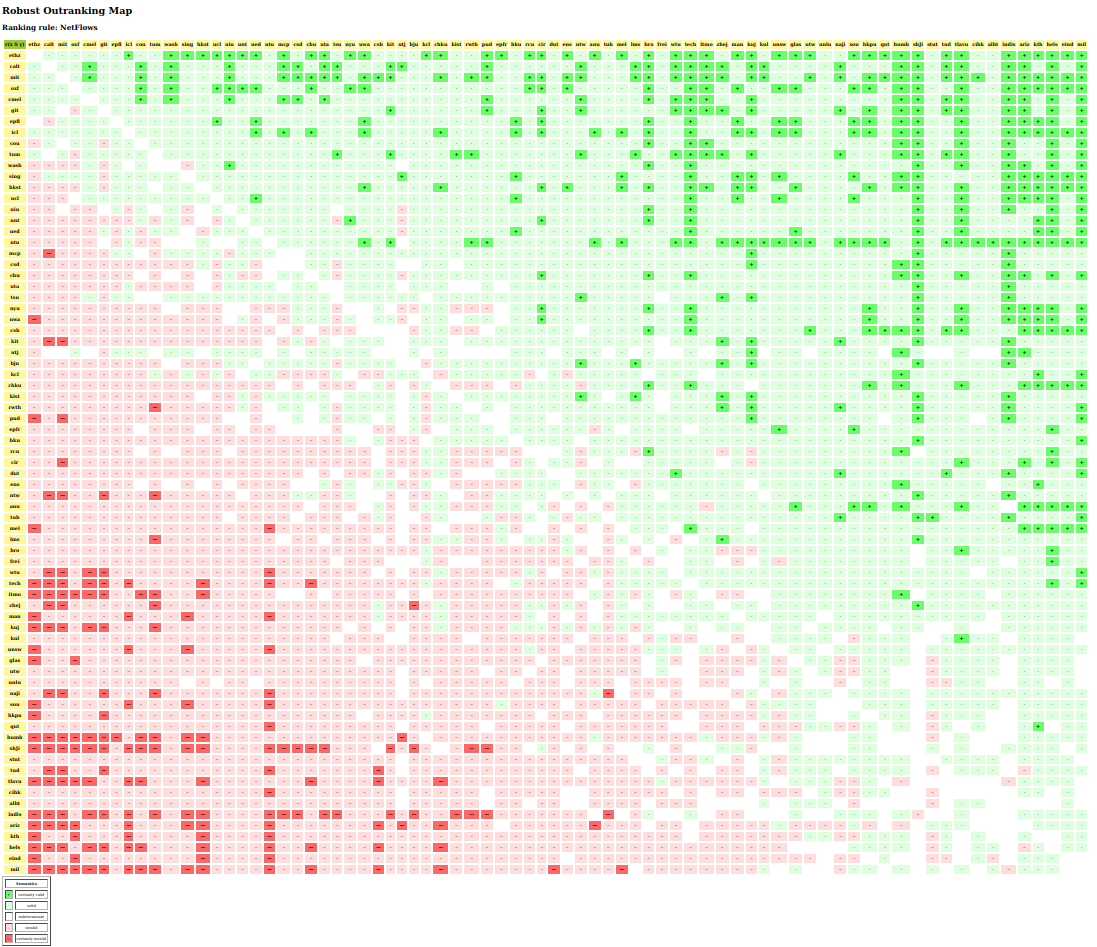
\includegraphics[width=\hsize]{Figures/13-2-the_cs_RelationMap.png}
\caption{Relation map of the robust outranking relation}
\label{fig:13.2}       % Give a unique label
\end{figure}

In Figure~\vref{fig:13.2}, \emph{dark green}, resp. \emph{light green} marked positions show certainly, resp. positively valid outranking situations, whereas \emph{dark red}, resp. \emph{light red} marked positions show certainly, respectively positively valid outranked situations. In the left upper corner one may verify that the five top-ranked Depts ([\texttt{ethz}, \texttt{calt}, \texttt{oxf}, \texttt{mit}, \texttt{cmel}]) are in fact mutually outranking each other and thus are all indifferent one to another. They give even robust \Condorcet winners by robustly outranking all other Depts.

Notice by the way that no certainly valid robust outranking (dark green) and no certainly valid robust outranked situations (dark red) appear in Figure~\vref{fig:13.3} below, resp. above the principal diagonal; none of these robust preferential situations are hence violated by the robust \NetFlows ranking. The non reflexive \emph{white} positions in the relation map, like the one between the Georgia Institute of Technology and the MIT, mark outranking or outranked situations that are not robust with respect to the given significance weight preorder. They become, hence, doubtful and are set to the indeterminate characteristic value $0.0$.

By measuring the ordinal correlation with the underlying pairwise global and marginal robust outranking situations, the quality of the robust \NetFlows ranking result can be formally evaluated with the \texttt{computeRankingCorrelation()} method\index{computeRankingCorrelation@\texttt{computeRankingCorrelation()}} and the \texttt{showCorrelation()} method\index{showCorrelation@\texttt{showCorrelation()}} (see Chap.~\ref{sec:16}).
\begin{lstlisting}[caption={Measuring the quality of the \NetFlows ranking result},label=list:13.12]
>>> corrnf = rdg.computeRankingCorrelation(nfRanking)
>>> rdg.showCorrelation(corrnf)   
  Correlation indexes:
    Crisp ordinal correlation  : +0.901
    Epistemic determination    :  0.563
    Bipolar-valued equivalence : +0.507
\end{lstlisting}

Listing~\vref{list:13.12} Line 4 indicates that the \NetFlows ranking result is indeed highly ordinally correlated ($+0.901$, in \Kendall 's tau index sense) with the pairwise global robust outranking relation. Their bipolar-valued \emph{relational equivalence} index ($+0.51$, Line 6) indicates a more than $75\%$ criteria significance support.

With the \texttt{showRankingConsensusQuality()} method,  we can also check how the \NetFlows ranking rule is actually balancing the five ranking objectives.\index{showRankingConsensusQuality@\texttt{showRankingConsensusQuality()}}
\begin{lstlisting}[caption={Measuring the consensus quality of the \NetFlows ranking result},label=list:13.13]
>>> rdg.showRankingConsensusQuality(nfRanking)
  Criterion (weight): correlation
  -------------------------------
    gtch (0.300): +0.660
    gres (0.300): +0.638
    gcit (0.275): +0.370
    gint (0.075): +0.155
    gind (0.050): +0.101
   Summary:
    Weighted mean marginal correlation (a): +0.508
    Standard deviation (b)                : +0.187
    Ranking fairness (a)-(b)              : +0.321
\end{lstlisting}

The ordinal correlation indexes with the marginal performance criterion rankings are nearly respecting the given significance weights preorder: \texttt{gtch} $\approx$ \texttt{gres} $>$ \texttt{gcit} $>$ \texttt{gint} $>$ \texttt{gind} (see Lines 4-8 above). The mean marginal ordinal correlation index is quite high ($+0.51$). Coupled with a low standard deviation ($0.187$), we obtain a quite fairly balanced ranking result (Lines 10-12). 

We can furthermore inspect with the \texttt{showCriteriaCorrelationTable()} method \index{showCriteriaCorrelationTable@\texttt{showCriteriaCorrelationTable()}} the mutual correlation indexes observed between the individual criterion based marginal robust outranking relations. 
\begin{lstlisting}[caption={Showing the ordinal correlation between the marginal criterion relations},label=list:13.13]
>>> rdg.showCriteriaCorrelationTable()
    Criteria ordinal correlation index
	 |  gcit    gind    gint    gres    gtch   
    -----|------------------------------------------
    gcit | +1.00   -0.11   +0.24   +0.13   +0.17   
    gind |         +1.00   -0.18   +0.15   +0.15   
    gint |                 +1.00   +0.04   -0.00   
    gres |                         +1.00   +0.67   
    gtch |                                 +1.00   
\end{lstlisting}

Slightly contradictory ($-0.11$) appear the \emph{Citations} and \emph{Industrial income} criteria (Line 5 Column 3 in List.~\vref{list:13.13}). Due perhaps to potential confidentiality clauses, it seams perhaps not always possible to publish industrially relevant research results in highly ranked journals. However, criteria \emph{Citations} and \emph{International outlook} show a slightly positive correlation ($+0.24$, Column 4), whereas the \emph{International outlook} criterion shows no apparent correlation with both the major \emph{Teaching} and \emph{Research} criteria. The latter are however highly correlated ($+0.67$. Line 9 Column 6).

A Principal Component Analysis may well illustrate with the \texttt{export3Dplot\-OfCriteriaCorrelation()} method the previous findings \citep[Lecture 2]{CPSTAT-2020}. \index{export3DplotOfCriteriaCorrelation@\texttt{export3DplotOfCriteriaCorrelation()}}
\begin{lstlisting}
>>> rdg.export3DplotOfCriteriaCorrelation(graphType='pdf')
\end{lstlisting}
\begin{figure}[ht]
%\sidecaption
\includegraphics[width=\hsize]{Figures/13-3-3DCorrelation.pdf}
\caption{3D PCA plot of the pairwise criteria correlation table.}
\label{fig:13.3}       % Give a unique label
\end{figure}

In Figure~\vref{fig:13.3}, one may notice first that more than $80\%$ of the total variance of the previous correlation table is explained by the apparent opposition between the marginal outrankings of criteria: \emph{Teaching}, \emph{Research} and \emph{Industry income} on the left side, and the marginal outrankings of criteria: \emph{Citations} and \emph{International outlook} on the right side. Notice also in the left lower corner the nearly identical positions of the marginal outrankings of the major \emph{Teaching} and \emph{Research} criteria. In the factors 2 and 3 plot, about $30\%$ of the total variance is captured by the opposition between the marginal outrankings of the \emph{Teaching} and \emph{Research} criteria and the marginal outrankings of the \emph{Industrial income} criterion. Finally, in the factors 1 and 3 plot, nearly $15\%$ of the total variance is explained by the opposition between the marginal outrankings of the \emph{International outlook} criterion and the marginal outrankings of the \emph{Citations} criterion.

It is, finally, interesting to similarly assess the ordinal correlation between the THE average scores-based ranking and the robust outranking digraph.
\begin{lstlisting}[caption={Computing the ordinal quality of the THE ranking},label=list:13.14]
>>> # theScores = [(xScore_1,x_1), (xScore_2,x_2),... ]
>>> # is sorted in decreasing order of xscores
>>> theRanking = [item[1] for item in theScores]
>>> corrthe = rdg.computeRankingCorrelation(theRanking)
>>> rdg.showCorrelation(corrthe)
    Correlation indexes:
     Crisp ordinal correlation  : +0.907
     Epistemic determination    :  0.563
     Bipolar-valued equivalence : +0.511
>>> rdg.showRankingConsensusQuality(theRanking)
    Criterion (weight): correlation
    -------------------------------
     gtch (0.300): +0.683
     gres (0.300): +0.670
     gcit (0.275): +0.319
     gint (0.075): +0.161
     gind (0.050): +0.106
    Summary:
     Weighted mean marginal correlation (a): +0.511
     Standard deviation (b)                : +0.210
     Ranking fairness (a)-(b)              : +0.302
\end{lstlisting}

The THE ranking result is similarly correlated ($+0.907$, Line 7 in Listing~\ref{list:13.14}) with the pairwise global robust outranking situations. By its overall weighted scoring rule, the THE ranking natuarlly induces marginal criterion correlations that are compatible with the given significance weight preorder (Lines 13-17). Notice that the mean marginal correlation is of a similar value ($+0.51$, Line 19) as the robust \NetFlows ranking. Yet, its standard deviation is slightly higher, which leads to a less fairer balancing of the three major ranking criteria.

To conclude, let us emphasize, that, without any commensurability hypothesis and by taking, furthermore, into account, first, the always present more or less imprecision of any performance grading and, secondly, solely ordinal criteria significance weights, we may obtain here with our robust outranking approach a very similar ranking result with a slightly better preference modelling quality. A convincing heatmap view of the 25 first-ranked Institutions may eventually be generated in the default system browser with following command.
\begin{lstlisting}
>>> rdg.showHTMLPerformanceHeatmap(
...            WithActionNames=True,\
...            outrankingModel='this',\
...            rankingRule='NetFlows',\
...            ndigits=1,\
...            Correlations=True,\
...            fromIndex=0,toIndex=25)
\end{lstlisting}
\begin{figure}[h]
%\sidecaption
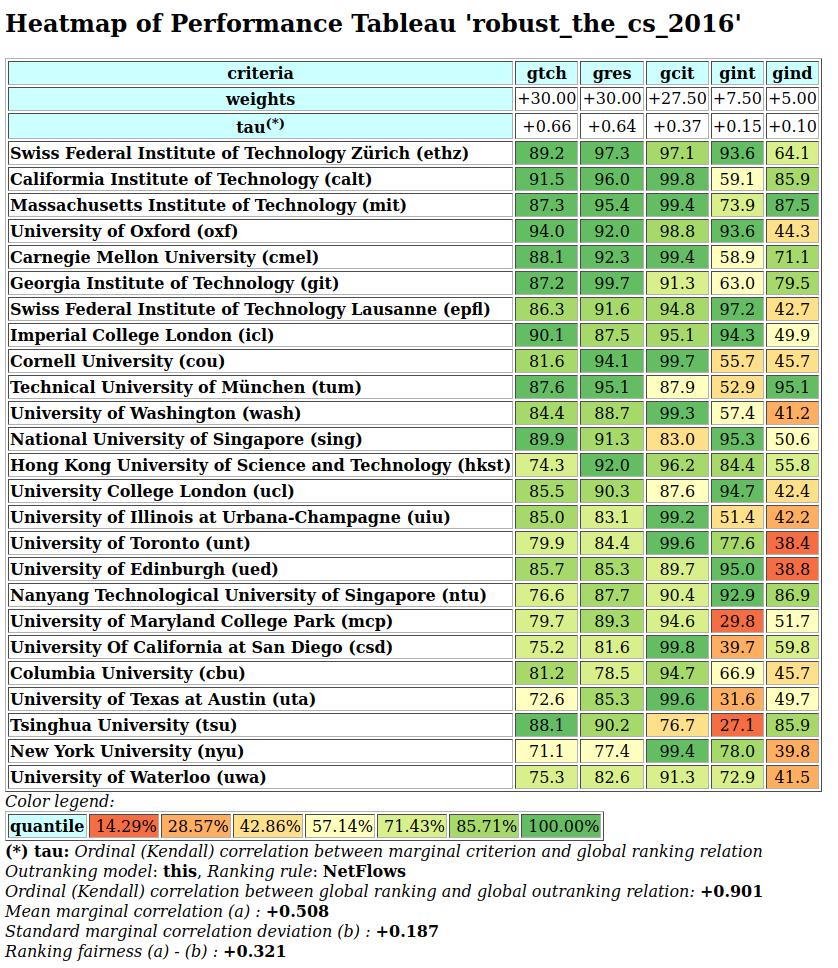
\includegraphics[width=\hsize]{Figures/13-4-theHeatmap.png}
\caption{Extract of a heatmap browser view on the \NetFlows ranking result}
\label{fig:13.4}       % Give a unique label
\end{figure}

As an exercise, the reader is invited to try out other robust outranking based ranking heuristics. Notice also that we have not challenged in this case study the THE provided criteria significance preorder. It would be very interesting to consider the five ranking objectives as equally important and, consequently, consider the ranking criteria to be equisignificant. Curious to see the ranking results under such settings.
 
%%%%%%% The chapter bibliography
%\normallatexbib
\clearpage
%\phantomsection
%\addcontentsline{toc}{section}{Chapter Bibliography}
\bibliographystyle{spbasic}
%\typeout{}
\bibliography{03-backMatters/reference}
%\chapter{The best academic Computer Science Depts: A ranking case study}
\label{sec:13}

\abstract*{ In this case study, we are solving with our \Digraph resources a ranking decision problem based on published data from the \emph{Times Higher Education} (THE) \emph{World University Rankings} 2016 by \emph{Computer Science} (CS) subject. Several hundred academic CS Departments, from all over the world, were ranked that year following an overall numerical score based on the weighted average of five performance criteria: \emph{Teaching} (the learning environment, $30\%$), \emph{Research} (volume, income and reputation, $30\%$), \emph{Citations} (research influence, $27.5\%$), \emph{International outlook} (staff, students, and research, $7.5\%$), and \emph{Industry income} (innovation, $5\%$). To illustrate our \Digraph programming resources, we shall first have a look into the THE ranking data with short Python scripts. In a second section, we shall relax the commensurability hypothesis of the ranking criteria and show how to similarly rank with multiple incommensurable performance criteria of solely ordinal significance. A third Section is finally devoted to introduce quality measures for qualifying ranking results.}

\abstract{ In this case study, we are solving with our \Digraph resources a ranking decision problem based on published data from the \emph{Times Higher Education} (THE) \emph{World University Rankings} 2016 by \emph{Computer Science} (CS) subject. Several hundred academic CS Departments, from all over the world, were ranked that year following an overall numerical score based on the weighted average of five performance criteria: \emph{Teaching} (the learning environment, $30\%$), \emph{Research} (volume, income and reputation, $30\%$), \emph{Citations} (research influence, $27.5\%$), \emph{International outlook} (staff, students, and research, $7.5\%$), and \emph{Industry income} (innovation, $5\%$). To illustrate our \Digraph programming resources, we shall first have a look into the THE multiple-criteria ranking data with short Python scripts. In a second section, we shall relax the commensurability hypothesis of the ranking criteria and show how to similarly rank with multiple incommensurable performance criteria of solely ordinal significance. A third section is finally devoted to introduce quality measures for qualifying ranking results.
}

\section{The THE performance tableau}
\label{sec:13.1}

For this decision making case study, we use an extract of the published \THE (THE) World University rankings 2016 by Computer Science (CS) subject, concerning the 75 first-ranked academic Institutions\footnote{\href{https://www.timeshighereducation.com/world-university-rankings/2017/subject-ranking/computer-science}{THE World University Rankings 2016 by Computer Science subject}}. The multiple-criteria performance tableau data, collected from the THE web pages, is stored in a file named \texttt{the-cs-2016.py} of \texttt{PerformanceTableau} format \footnote{The performance tableau \texttt{the-cs-2016.py} is available in the \texttt{examples} directory of the \Digraph resources \citep{BIS-2021}.}.\index{THE University rankings 2016 by CS subject} 
\begin{lstlisting}[caption={Performance tableau of the },label=list:13.1]
>>> from perfTabs import PerformanceTableau
>>> cspt = PerformanceTableau('the_cs_2016')
>>> cspt
  *------- PerformanceTableau instance description ------*
   Instance class     : PerformanceTableau
   Instance name      : the-cs-2016
   Actions            : 75
   Objectives         : 5
   Criteria           : 5
   NaN proportion (%) : 0.0
   Attributes         : ['name','description','actions',
                           'objectives','criteria',
			   'weightPreorder','NA','evaluation']
\end{lstlisting}

Potential decision alternatives, in our case here, are the 75 THE best-ranked CS Departments in 2016, all of them located at world renowned Institutions, like California Institute of Technology, Swiss Federal Institute of Technology Zurich, Technical University München, University of Oxford or the National University of Singapore (see List.~\vref{list:13.2} below). 

Instead of using prefigured \Digraph \texttt{show...()} methods, readily available for inspecting \texttt{PerformanceTableau} instances, Listing~\vref{list:13.2} illustrates how to write small Python scripts for printing out its content.   
\begin{lstlisting}[caption={Printing the CS Departments},label=list:13.2,basicstyle=\ttfamily\scriptsize]
>>> for x in cspt.actions:
...     print('%s:\t%s (%s)' %\
...        (x,cspt.actions[x]['name'],cspt.actions[x]['comment']) )
  albt:	University of Alberta (CA)
  anu:	Australian National University (AU)
  ariz:	Arizona State University (US)
  bju:	Beijing University (CN)
  bro:	Brown University (US)
  calt:	California Institute of Technology (US)
  cbu:	Columbia University (US)
  chku:	Chinese University of Hong Kong (HK)
  cihk:	City University of Hong Kong (HK)
  cir:	University of California at Irvine (US)
  cmel:	Carnegie Mellon University (US)
  cou:	Cornell University (US)
  csb:	University of California at Santa Barbara (US)
  csd:	University Of California at San Diego (US)
  dut:	Delft University of Technology (NL)
  eind:	Eindhoven University of Technology (NL)
  ens:	Superior Normal School at Paris (FR)
  epfl:	Swiss Federal Institute of Technology Lausanne (CH)
  epfr:	Polytechnic school of Paris (FR)
  ethz:	Swiss Federal Institute of Technology Zurich (CH)
  frei:	University of Freiburg (DE)
  git:	Georgia Institute of Technology (US)
  glas:	University of Glasgow (UK)
  hels:	University of Helsinki (FI)
  hkpu:	Hong Kong Polytechnic University (CN)
  hkst:	Hong Kong University of Science and Technology (HK)
  hku:	Hong Kong University (HK)
  humb:	Berlin Humboldt University (DE)
  icl:	Imperial College London (UK)
  indis:Indian Institute of Science (IN)
  itmo:	ITMO University (RU)
  kcl:	King's College London (UK)
  kist:	Korea Adv. Institute of Science and Technology (KR)
  kit:	Karlsruhe Institute of Technology (DE)
  kth:	KTH Royal Institute of Technology (SE)
  kuj:	Kyoto University (JP)
  kul:	Catholic University Leuven (BE)
  lms:	Lomonosov Moscow State University (RU)
  man:	University of Manchester (UK)
  mcp:	University of Maryland College Park (US)
  mel:	University of Melbourne (AU)
  mil:	Polytechnic University of Milan (IT)
  mit:	Massachusetts Institute of Technology (US)
  naji:	Nanjing University (CN)
  ntu:	Nanyang Technological University of Singapore (SG)
  ntw:	National Taiwan University (TW)
  nyu:	New York University (US)
  oxf:	University of Oxford (UK)
  pud:	Purdue University (US)
  qut:	Queensland University of Technology (AU)
  rcu:	Rice University (US)
  rwth:	RWTH Aachen University (DE)
  shJi:	Shanghai Jiao Tong University (CN)
  sing:	National University of Singapore (SG)
  sou:	University of Southhampton (UK)
  stut:	University of Stuttgart (DE)
  tech:	Technion - Israel Institute of Technology (IL)
  tlavu:Tel Aviv University (IR)
  tsu:	Tsinghua University (CN)
  tub:	Technical University of Berlin (DE)
  tud:	Technical University of Darmstadt (DE)
  tum:	Technical University of Muenchen (DE)
  ucl:	University College London (UK)
  ued:	University of Edinburgh (UK)
  uiu:	University of Illinois at Urbana-Champagne (US)
  unlu:	University of Luxembourg (LU)
  unsw:	University of New South Wales (AU)
  unt:	University of Toronto (CA)
  uta:	University of Texas at Austin (US)
  utj:	University of Tokyo (JP)
  utw:	University of Twente (NL)
  uwa:	University of Waterloo (CA)
  wash:	University of Washington (US)
  wtu:	Vienna University of Technology (AUS)
  zhej:	Zhejiang University (CN)
\end{lstlisting}

The THE authors base their 2016 ranking on five decision objectives \citep{THE-2016}.
\begin{lstlisting}[caption={The THE ranking objectives},label=list:13.3,basicstyle=\ttfamily\scriptsize]
>>> for obj in cspt.objectives:
...     print('%s: %s (%.1f%%),\n\t%s' %\
...                (obj,cspt.objectives[obj]['name'],\
...                 cspt.objectives[obj]['weight'],
...                 cspt.objectives[obj]['comment'])\
...           ) 
 Teaching: Best learning environment (30.0%)
   Reputation survey; Staff-to-student ration;
   Doctorate-to-student ratio;
   Doctorate-to-academic-staff ratio;
   Institutional income.
 Research: Highest volume and reputation (30.0%)
   Reputation survey;
   Research income;
   Research productivity.
 Citations: Highest research influence (27.5%)
   Impact.
 International outlook: Most international staff,
                        students and research (7.5%)
   Proportions of international students;
   Proportions of international staff;
   International collaborations.
 Industry income: Best knowledge transfer (5.0%)
   Volume.
\end{lstlisting}

With a cumulated importance of $87\%$ (see above), \emph{Teaching}, \emph{Research} and \emph{Citations} represent clearly the major ranking objectives. \emph{International outlook} and \emph{Industry income} are considered of minor importance ($12.5\%$).

THE authors do, unfortunately, not publish the detail of their performance assessments for evaluating CS Depts with respect to each one of performance criteria per ranking objective.  \footnote{THE gives some insight on the subject and significance of the actual ranking criteria used for evaluating along each ranking objective on her website \citep{THE-2016}}. The THE 2016 ranking publication reveals solely a compound assessment on a single performance criteria per ranking objective. The five retained performance criteria may be printed out as follows.
\begin{lstlisting}
>>> for g in cspt.criteria:
...     print('%s:\t%s, %s (%.1f%%)' %\
...       (g,cspt.criteria[g]['name'],cspt.criteria[g]['comment'],\
...        cspt.criteria[g]['weight']) )  
  gtch:	Teaching, The learning environment (30.0%)
  gres:	Research, Volume, income and reputation (30.0%)
  gcit:	Citations, Research influence (27.5%)
  gint:	International outlook, In staff, students and research (7.5%)
  gind:	Industry income, knowledge transfer (5.0%)
\end{lstlisting}

The largest part ($87.5\%$) of criteria significance is, hence canonically, allocated to the major ranking criteria: \emph{Teaching} ($30\%$), \emph{Research} ($30\%$) and \emph{Citations} ($27.5\%$). The small remaining part ($12.5\%$) goes to \emph{International outlook} ($7.5\%$) and \emph{Industry income} ($5\%$).

In order to render commensurable these performance criteria, the THE authors replace, per criterion, the actual performance evaluation obtained by each University with the corresponding \emph{quantile} observed in the cumulative distribution of the performance evaluations obtained by all the surveyed institutions \citep{THE-2016}. The THE ranking is eventually determined by an \emph{overall score} per University which corresponds to the weighted average of these five criteria quantiles, as illustrated in Listing~\vref{list:13.4}.     
\begin{lstlisting}[caption={Computing the THE overall scores},label=list:13.4]
>>> theScores = []
>>> for x in cspt.actions:
...     xscore = Decimal('0')
...     for g in cspt.criteria:
...         xscore += cspt.evaluation[g][x] *\
...          (cspt.criteria[g]['weight']/Decimal('100'))
...	   theScores.append((xscore,x))
\end{lstlisting}

In Listing~\vref{list:13.5} (Lines 15-16), we may thus notice that, in the 2016 edition of the THE World University rankings by CS subject, the Swiss Federal Institute of Technology Zürich is first-ranked with an overall score of $92.9$; followed by the California Institute of Technology (overall score: $92.4$) \footnote{The author's own Computer Science Dept at the University of Luxembourg was ranked on position 63 with an overall score of $58.0$.}.
\begin{lstlisting}[caption={Printing the ranked performance table},label=list:13.5,basicstyle=\ttfamily\scriptsize]
>>> theScores.sort(reverse = True)
>>> print('##  Univ \tgtch  gres  gcit  gint  gind  overall')
>>> print('-------------------------------------------------') 
>>> i = 1
>>> for it in theScores:
...     x = it[1]
...     xScore = it[0]
...     print('%2d: %s' % (i,x), end=' \t')
...     for g in cspt.criteria:
...         print('%.1f ' % (cspt.evaluation[g][x]),end=' ')
...	    print(' %.1f' % xScore)
...         i += 1   
    ##  Univ 	gtch  gres  gcit  gint  gind  overall
    -------------------------------------------------
     1: ethz 	89.2  97.3  97.1  93.6  64.1   92.9
     2: calt 	91.5  96.0  99.8  59.1  85.9   92.4
     3: oxf 	94.0  92.0  98.8  93.6  44.3   92.2
     4: mit 	87.3  95.4  99.4  73.9  87.5   92.1
     5: git 	87.2  99.7  91.3  63.0  79.5   89.9
     6: cmel 	88.1  92.3  99.4  58.9  71.1   89.4
     7: icl 	90.1  87.5  95.1  94.3  49.9   89.0
     8: epfl 	86.3  91.6  94.8  97.2  42.7   88.9
     9: tum 	87.6  95.1  87.9  52.9  95.1   87.7
    10: sing 	89.9  91.3  83.0  95.3  50.6   86.9
    11: cou 	81.6  94.1  99.7  55.7  45.7   86.6
    12: ucl 	85.5  90.3  87.6  94.7  42.4   86.1
    13: wash 	84.4  88.7  99.3  57.4  41.2   85.6
    14: hkst 	74.3  92.0  96.2  84.4  55.8   85.5
    15: ntu 	76.6  87.7  90.4  92.9  86.9   85.5
    16: ued 	85.7  85.3  89.7  95.0  38.8   85.0
    17: unt 	79.9  84.4  99.6  77.6  38.4   84.4
    18: uiu 	85.0  83.1  99.2  51.4  42.2   83.7
    19: mcp 	79.7  89.3  94.6  29.8  51.7   81.5
    20: cbu 	81.2  78.5  94.7  66.9  45.7   81.3
    21: tsu 	88.1  90.2  76.7  27.1  85.9   80.9
    22: csd 	75.2  81.6  99.8  39.7  59.8   80.5
    23: uwa 	75.3  82.6  91.3  72.9  41.5   80.0
    24: nyu 	71.1  77.4  99.4  78.0  39.8   79.7
    25: uta 	72.6  85.3  99.6  31.6  49.7   79.6
    26: kit 	73.8  85.5  84.4  41.3  76.8   77.9
    27: bju 	83.0  85.3  70.1  30.7  99.4   77.0
    28: csb 	65.6  70.9  94.8  72.9  74.9   76.2
    29: rwth 	77.8  85.0  70.8  43.7  89.4   76.1
    30: hku 	77.0  73.0  77.0  96.8  39.5   75.4
    31: pud 	76.9  84.8  70.8  58.1  56.7   75.2
    32: kist 	79.4  88.2  64.2  31.6  92.8   74.9
    33: kcl 	45.5  94.6  86.3  95.1  38.3   74.8
    34: chku 	64.1  69.3  94.7  75.6  49.9   74.2
    35: epfr 	81.7  60.6  78.1  85.3  62.9   73.7
    36: dut 	64.1  78.3  76.3  69.8  90.1   73.4
    37: tub 	66.2  82.4  71.0  55.4  99.9   73.3
    38: utj 	92.0  91.7  48.7  25.8  49.6   72.9
    39: cir 	68.8  64.6  93.0  65.1  40.4   72.5
    40: ntw 	81.5  79.8  66.6  25.5  67.6   72.0
    41: anu 	47.2  73.0  92.2  90.0  48.1   70.6
    42: rcu 	64.1  53.8  99.4  63.7  46.1   69.8
    43: mel 	56.1  70.2  83.7  83.3  50.4   69.7
    44: lms 	81.5  68.1  61.0  31.1  87.8   68.4
    45: ens 	71.8  40.9  98.7  69.6  43.5   68.3
    46: wtu 	61.8  73.5  73.7  51.9  62.2   67.9
    47: tech 	54.9  71.0  85.1  51.7  40.1   67.1
    48: bro 	58.5  54.9  96.8  52.3  38.6   66.5
    49: man 	63.5  71.9  62.9  84.1  42.1   66.3
    50: zhej 	73.5  70.4  60.7  22.6  75.7   65.3
    51: frei 	54.2  51.6  89.5  49.7  99.9   65.1
    52: unsw 	60.2  58.2  70.5  87.0  44.3   63.6
    53: kuj 	75.4  72.8  49.5  28.3  51.4   62.8
    54: sou 	48.2  60.7  75.5  87.4  43.2   62.1
    55: shJi 	66.9  68.3  62.4  22.8  38.5   61.4
    56: itmo 	58.0  32.0  98.7  39.2  68.7   60.5
    57: kul 	35.2  55.8  92.0  46.0  88.3   60.5
    58: glas 	35.2  52.5  91.2  85.8  39.2   59.8
    59: utw 	38.2  52.8  87.0  69.0  60.0   59.4
    60: stut 	54.2  60.6  61.1  36.3  97.8   58.9
    61: naji 	51.4  76.9  48.8  39.7  74.4   58.6
    62: tud 	46.6  53.6  75.9  53.7  66.5   58.3
    63: unlu 	35.2  44.2  87.4  99.7  54.1   58.0
    64: qut 	45.5  42.6  82.8  75.2  63.0   58.0
    65: hkpu 	46.8  36.5  91.4  73.2  41.5   57.7
    66: albt 	39.2  53.3  69.9  91.9  75.4   57.6
    67: mil 	46.4  64.3  69.2  44.1  38.5   57.5
    68: hels 	48.8  49.6  80.4  50.6  39.5   57.4
    69: cihk 	42.4  44.9  80.1  76.2  67.9   57.3
    70: tlavu 	34.1  57.2  89.0  45.3  38.6   57.2
    71: indis 	56.9  76.1  49.3  20.1  41.5   57.0
    72: ariz 	28.4  61.8  84.3  59.3  42.0   56.8
    73: kth 	44.8  42.0  83.6  71.6  39.2   56.4
    74: humb 	48.4  31.3  94.7  41.5  45.5   55.3
    75: eind 	32.4  48.4  81.5  72.2  45.8   54.4
\end{lstlisting}

It is important to notice that a ranking by weighted average scores requires \emph{commensurable ranking criteria} of precise decimal significance and on wich precise decimal performance evaluations are given. It is very unlikely that the THE 2016 performance assessments verify indeed these conditions. Here we show how to relax these methodological requirements --precise commensurable criteria and decimal evaluations-- by following instead a bipolar-valued epistemic logic based ranking methodology (see Chap.~\ref{sec:8}).

\section{Ranking with multiple criteria of ordinal significance}
\label{sec:13.2}

Let us, first, have a critical look in Figure~\vref{fig:13.1} at the THE performance criteria.
\begin{lstlisting}
>>> cspt.showHTMLCriteria(Sorted=False)
\end{lstlisting}
\begin{figure}[ht]
%\sidecaption
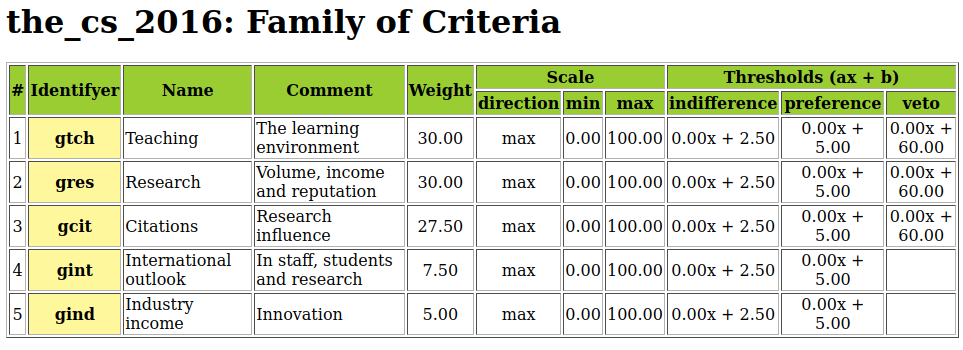
\includegraphics[width=\hsize]{Figures/13-1-the_cs_2016Criteria.png}
\caption{The THE ranking criteria}
\label{fig:13.1}       % Give a unique label
\end{figure}

Considering a very likely imprecision of the performance evaluation procedure, followed by some potential violation of uniform distributed quantile classes, we assume here that a performance quantile difference of up to $2.5\%$ is \emph{insignificant}, whereas a difference of $5\%$ and more warrants a \emph{clearly better}, resp. \emph{clearly less good} performance. With quantiles $94\%$, resp. $87.3\%$, Oxford's CS teaching environment, for instance, is thus clearly better evaluated than that of the MIT (see List.~\vref{list:13.5} Lines 27-28). We shall furthermore assume that a \emph{considerable} performance quantile difference of $60\%$, observed on the three major ranking criteria: \emph{Teaching}, \emph{Research} and \emph{Citations}, will trigger the polarisation of pairwise outranking, respectively outranked situations \citep{BIS-2013}.

The effect these performance discrimination thresholds induce on the outranking modelling can be inspected with the \texttt{showCriteria()} method\index{showCriteria@\texttt{showCriteria()}}.
\begin{lstlisting}[caption={Inspecting the performance discrimination thresholds},label=list:13.6]
>>> cspt.showCriteria()
  *----  criteria -----*
    gtch 'Teaching'
      Scale = (Decimal('0.00'), Decimal('100.00'))
      Weight = 0.300 
      Threshold ind : 2.50 + 0.00x ;   percentile:  8.07
      Threshold pref : 5.00 + 0.00x ;  percentile: 15.75
      Threshold veto : 60.00 + 0.00x ; percentile: 99.75
    gres 'Research'
      Scale = (Decimal('0.00'), Decimal('100.00'))
      Weight = 0.300 
      Threshold ind : 2.50 + 0.00x ;   percentile:  7.86
      Threshold pref : 5.00 + 0.00x ;  percentile: 16.14
      Threshold veto : 60.00 + 0.00x ; percentile: 99.21
    gcit 'Citations'
      Scale = (Decimal('0.00'), Decimal('100.00'))
      Weight = 0.275 
      Threshold ind : 2.50 + 0.00x ;   percentile:  11.82
      Threshold pref : 5.00 + 0.00x ;  percentile:  22.99
      Threshold veto : 60.00 + 0.00x ; percentile: 100.00
    gint 'International outlook'
      Scale = (Decimal('0.00'), Decimal('100.00'))
      Weight = 0.075 
      Threshold ind : 2.50 + 0.00x ;  percentile:  6.45
      Threshold pref : 5.00 + 0.00x ; percentile: 11.75
    gind 'Industry income'
      Scale = (Decimal('0.00'), Decimal('100.00'))
      Weight = 0.050 
      Threshold ind : 2.50 + 0.00x ;  percentile: 11.82
      Threshold pref : 5.00 + 0.00x ; percentile: 21.51
\end{lstlisting}

Between $6\%$ and $12\%$ of the observed quantile differences are, hence, considered to be \emph{insignificant}. Similarly, between $77\%$ and $88\%$ are considered to be \emph{significant}. Less than $1\%$ correspond to \emph{considerable} quantile differences on both the \emph{Teaching} and \emph{Research} criteria; actually triggering an epistemic polarisation effect \citep{BIS-2013}.

Beside the likely imprecise performance discrimination, the \emph{precise decimal significance weights}, as allocated by the THE authors to the five ranking criteria are, as well, quite \emph{questionable}. Criteria significance weights may carry sometimes hidden strategies for rendering the performance evaluations commensurable in view of a numerical computation of the overall ranking scores. The eventual ranking result is, the case given, as much depending on the precise values of the given criteria significance weights as, vice versa, the given precise significance weights are depending on the subjectively expected and accepted ranking results \footnote{In a social choice context, this potential double bind between voting profiles and election result, corresponds to voting manipulation strategies.}. We will therefore drop these precise decimal weights and, instead, only require a corresponding criteria significance preorder: \texttt{gtch} $=$ \texttt{gres} $>$ \texttt{gcit} $>$ \texttt{gint} $>$ \texttt{gind}. \emph{Teaching environment} and \emph{Research volume and reputation} are equally considered most significant, followed by \emph{Research influence}. Then comes \emph{International outlook in staff, students and research} and, least significant finally, \emph{Industry income and innovation}.

Both these working hypotheses: --performance discrimination thresholds and --solely ordinal criteria significance, give us way to a ranking methodology based on \emph{robust pairwise outranking} situations (see Chap.~\ref{sec:19} and \citep{BIS-2004b}).
\begin{definition}[Robust outranking situations with ordinal criteria significance weights]\label{def:13.1}
\begin{itemize}[topsep=1pt]
\item We say that CS Dept $x$ \emph{robustly outranks} CS Dept $y$ when $x$ positively outranks $y$ with \textbf{all} significance weight vectors that are compatible with the significance preorder: \texttt{gtch} $=$ \texttt{gres} $>$ \texttt{gcit} $>$ \texttt{gint} $>$ \texttt{gind};
\item We say that CS Dept $x$ is \emph{robustly outranked} by CS Dept $y$ when $x$ is positively outranked by $y$ with \textbf{all} significance weight vectors that are compatible with the significance preorder: \texttt{gtch} $=$ \texttt{gres} $>$ \texttt{gcit} $>$ \texttt{gint} $>$ \texttt{gind};
\item Otherwise, CS Depts $x$ and $y$ are considered to be \emph{incomparable}.
\end{itemize}
\end{definition}

A corresponding digraph constructor is provided by the \texttt{RobustOutranking\-Digraph} class\index{RobustOutrankingDigraph@\texttt{RobustOutrankingDigraph} class}.
\begin{lstlisting}[caption={Computing the robust outranking digraph},label=list:13.7]
>>> from outrankingDigraphs import RobustOutrankingDigraph	     
>>> rdg = RobustOutrankingDigraph(cspt)
>>> rdg
  *------- Object instance description ------*
   Instance class       : RobustOutrankingDigraph
   Instance name        : robust_the_cs_2016
   Actions              : 75
   Criteria             : 5
   Size                 : 2993
   Determinateness (%)  : 78.16
   Valuation domain     : [-1.00;1.00]
>>> rdg.computeIncomparabilityDegree(Comments=True)
  Incomparability degree (%) of digraph <robust_the_cs_2016>:
   links x<->y y: 2775, incomparable: 102, comparable: 2673
   (incomparable/links) =  0.037
>>> rdg.computeTransitivityDegree(Comments=True)
  Transitivity degree of digraph <robust_the_cs_2016>:
   triples x>y>z: 405150, closed: 218489, open: 186661
   (closed/triples) =  0.539
>>> rdg.computeSymmetryDegree(Comments=True)
  Symmetry degree (%) of digraph <robust_the_cs_2016>:
   arcs x>y: 2673, symmetric: 320, asymmetric: 2353
   (symmetric/arcs) =  0.12
\end{lstlisting}

In the resulting digraph instance \texttt{rdg} (see Line 9 in Listing~\vref{list:13.7}), we observe $2993$ such robust pairwise outranking situations validated with a mean significance of $78\%$ (Line 10). Unfortunately, in the case here, they do not deliver any complete linear ranking. The robust outranking digraph \texttt{rdg} contains 102 incomparability situations ($3.7\%$, Line 15); nearly half of its transitive closure is missing ($46.1\%$, Line 19) and $12\%$ of the positive outranking situations correspond in fact to symmetric indifference situations (Line 23).

Worse even, the digraph \texttt{rdg} admits a really high number of outranking circuits \footnote{The \texttt{computeChordlessCircuits()} and \texttt{showChordlessCircuits()} methods are separate because there are various methods available for enumerating the chordless circuits in a digraph \citep{BIS-2010}.}.\index{showChordlessCircuits@\texttt{showChordlessCircuits()}}
\begin{lstlisting}[caption={Inspecting outranking circuits},label=list:13.8]
>>> rdg.computeChordlessCircuits()
>>> rdg.showChordlessCircuits()
 *---- Chordless circuits ----*
  145 circuits.
  1:  ['albt','unlu','ariz','hels'], cred. : 0.300
  2:  ['albt','tlavu','hels'], cred. : 0.150
  3:  ['anu', 'man', 'itmo'], cred. : 0.250
  4:  ['anu', 'zhej', 'rcu'], cred. : 0.250
    ...
    ...
  82:  ['csb','epfr','rwth'], cred. : 0.250
  83:  ['csb','epfr','pud','nyu'], cred. : 0.250
  84:  ['csd','kcl','kist'], cred. : 0.250
    ...
    ...
  142:  ['kul','qut','mil'], cred. : 0.250
  143:  ['lms','rcu','tech'], cred. : 0.300
  144:  ['mil','stut','qut'], cred. : 0.300
  145:  ['mil','stut','tud'], cred. : 0.300
\end{lstlisting}

Among the 145 detected robust outranking circuits reported in Listing \vref{list:13.8}, we notice, for instance, two outranking circuits of length 4 (see circuits 1 and 83).

Let us inspect below the bipolar-valued robust outranking characteristics of the first circuit.
\begin{lstlisting}[caption={Showing the relation table with stability denotation},label=list:13.9]
>>> rdg.showRelationTable(actionsSubset=\
...         ['albt','unlu','ariz','hels'],\
...         Sorted=False) 
  * ---- Relation Table -----
   r/(stab)|  'albt' 'unlu' 'ariz' 'hels'   
      -----|-----------------------------
    'albt' |  +1.00  +0.30  +0.00  +0.00  
           |   (+4)   (+2)   (-1)   (-1)  
    'unlu' |  +0.00  +1.00  +0.40  +0.00  
           |   (+0)   (+4)   (+2)   (-1)  
    'ariz' |  +0.00  -0.12  +1.00  +0.40  
           |   (+1)   (-2)   (+4)   (+2)  
    'hels' |  +0.45  +0.00  -0.03  +1.00  
           |   (+2)   (+1)   (-2)   (+4)  
   Valuation domain: [-1.0; 1.0]
   Stability denotation semantics:
   +4|-4 : unanimous outranking | outranked situation;
   +2|-2 : outranking | outranked situation validated
      with all potential significance weights that are
      compatible with the given significance preorder;
   +1|-1 : validated outranking | outranked situation
      with the given significance weights;
     0   : indeterminate relational situation.
\end{lstlisting}

In Listing~\vref{list:13.9}, we notice that the robust outranking circuit \texttt{[albt,} \texttt{unlu,} \texttt{ariz,} \texttt{hels]}  will reappear with all potential criteria significance weight vectors that are compatible with given preorder: \texttt{gtch} $=$ \texttt{gres} $>$ \texttt{gcit} $>$ \texttt{gint} $>$ \texttt{gind}. Notice also the ($\pm 1$) marked outranking situations, like the one between \texttt{albt} and \texttt{ariz}. The statement that ``\emph{Arizona State University strictly  outranks University of Alberta}'' is in fact valid with the precise THE criteria significance weights, but not with all potential significance weights vectors that are compatible with the given significance preorder. All these ($\pm 1$)  marked outranking situations become hence \emph{doubtful} ($r(x \succsim y) = 0.00$) and the corresponding CS Depts, like University of Alberta and Arizona State University, become \emph{incomparable} in a robust outranking sense.  

Showing many incomparabilities and indifferences; not being transitive and containing many robust outranking circuits; all these relational characteristics, make that no ranking algorithm, applied to digraph \texttt{rdg}, does exist that would produce a \emph{unique} optimal linear ranking result. Methodologically, we are only left with ranking heuristics. In Chapter~\ref{sec:8} on ranking with multiple criteria we have now seen several potential heuristic ranking rules that can be used for ranking with an outranking digraph; yet, they may deliver potentially more or less diverging results. Considering the order of digraph \texttt{rdg} (75) and the largely unequal THE criteria significance weights, we rather opt, in this tutorial, for the \NetFlows ranking rule \footnote{The reader might try other ranking rules, like the \Copeland or \Kohler rules. Mind that the latter ranking-by-choosing rule is more complex (see Chap.~\ref{sec:8}).}. Its complexity in $O(n^2)$ is indeed quite tractable and, by avoiding potential \emph{tyranny of short majority} effects, the \NetFlows rule may specifically take the ranking criteria significance weights into a more fairly balanced account.

The \NetFlows ranking result of the CS Depts can be directly computed with the \texttt{computeNetFlowsRanking()} method\index{computeNetFlowsRanking@\texttt{computeNetFlowsRanking()}}. 
\begin{lstlisting}[caption={Computing a robust \NetFlows ranking},label=list:13.10]
>>> nfRanking = rdg.computeNetFlowsRanking()
>>> nfRanking
  ['ethz','calt','mit', 'oxf',  'cmel','git', 'epfl',
   'icl', 'cou', 'tum', 'wash', 'sing','hkst','ucl',
   'uiu', 'unt', 'ued', 'ntu',  'mcp', 'csd', 'cbu',
   'uta', 'tsu', 'nyu', 'uwa',  'csb', 'kit', 'utj',
   'bju', 'kcl', 'chku','kist', 'rwth','pud', 'epfr',
   'hku', 'rcu', 'cir', 'dut',  'ens', 'ntw', 'anu',
   'tub', 'mel', 'lms', 'bro',  'frei','wtu', 'tech',
   'itmo','zhej','man', 'kuj',  'kul', 'unsw','glas',
   'utw', 'unlu','naji','sou',  'hkpu','qut', 'humb',
   'shJi','stut','tud', 'tlavu','cihk','albt','indis',
   'ariz','kth', 'hels','eind', 'mil']
\end{lstlisting}

We actually obtain in Listing~\vref{list:13.10} a very similar ranking result as the one obtained with the THE average scores. The same group of seven Depts: \texttt{ethz}, \texttt{calt}, \texttt{mit}, \texttt{oxf}, \texttt{cmel}, \texttt{git} and \texttt{epfl}, is top-ranked. And a same group of Depts: \texttt{tlavu}, \texttt{cihk}, \texttt{indis}, \texttt{ariz}, \texttt{kth}, \texttt{hels}, \texttt{eind}, and \texttt{mil} appears at the end of the list.

We can print out the difference between the overall scores based THE ranking and the \NetFlows ranking above with the following short Python script, where we make use of an ordered Python dictionary with net-flow scores, stored in the \texttt{rdg.netFlowsRankingDict} attribute by the previous computation.
\begin{lstlisting}[caption={Comparing the robust \NetFlows ranking with the THE ranking},label=list:13.11,basicstyle=\ttfamily\scriptsize]
>>> # rdg.netFlowsRankingDict: ordered dictionary with net flow
>>> # scores stored in rdg by the computeNetFlowsRanking() method
>>> # theScores = [(xScore_1,x_1), (xScore_2,x_2),... ]
>>> # is sorted in decreasing order of xscores_i
>>> print(\
...  ' NetFlows ranking   gtch  gres  gcit  gint  gind   THE ranking')
>>> for i in range(75):
...     x = nfRanking[i]
...     xScore = rdg.netFlowsRankingDict[x]['netFlow']
...     thexScore,thex = theScores[i]
...     print('%2d: %s (%.2f) ' % (i+1,x,xScore), end=' \t')
...     for g in rdg.criteria:
...         print('%.1f ' % (t.evaluation[g][x]),end=' ')
...     print(' %s (%.2f)' % (thex,thexScore) )  
  NetFlows ranking   gtch  gres  gcit  gint  gind   THE ranking
   1: ethz (116.95)  89.2  97.3  97.1  93.6  64.1   ethz (92.88)
   2: calt (116.15)  91.5  96.0  99.8  59.1  85.9   calt (92.42)
   3: mit (112.72)   87.3  95.4  99.4  73.9  87.5   oxf (92.20)
   4: oxf (112.00)   94.0  92.0  98.8  93.6  44.3   mit (92.06)
   5: cmel (101.60)  88.1  92.3  99.4  58.9  71.1   git (89.88)
   6: git (93.40)    87.2  99.7  91.3  63.0  79.5   cmel (89.43)
   7: epfl (90.88)   86.3  91.6  94.8  97.2  42.7   icl (89.00)
   8: icl (90.62)    90.1  87.5  95.1  94.3  49.9   epfl (88.86)
   9: cou (84.60)    81.6  94.1  99.7  55.7  45.7   tum (87.70)
  10: tum (80.42)    87.6  95.1  87.9  52.9  95.1   sing (86.86)
  11: wash (76.28)   84.4  88.7  99.3  57.4  41.2   cou (86.59)
  12: sing (73.05)   89.9  91.3  83.0  95.3  50.6   ucl (86.05)
  13: hkst (71.05)   74.3  92.0  96.2  84.4  55.8   wash (85.60)
  14: ucl (66.78)    85.5  90.3  87.6  94.7  42.4   hkst (85.47)
  15: uiu (64.80)    85.0  83.1  99.2  51.4  42.2   ntu (85.46)
  16: unt (62.65)    79.9  84.4  99.6  77.6  38.4   ued (85.03)
  17: ued (58.67)    85.7  85.3  89.7  95.0  38.8   unt (84.42)
  18: ntu (57.88)    76.6  87.7  90.4  92.9  86.9   uiu (83.67)
  19: mcp (54.08)    79.7  89.3  94.6  29.8  51.7   mcp (81.53)
  20: csd (46.62)    75.2  81.6  99.8  39.7  59.8   cbu (81.25)
  21: cbu (44.27)    81.2  78.5  94.7  66.9  45.7   tsu (80.91)
  22: uta (43.27)    72.6  85.3  99.6  31.6  49.7   csd (80.45)
  23: tsu (42.42)    88.1  90.2  76.7  27.1  85.9   uwa (80.02)
  24: nyu (35.30)    71.1  77.4  99.4  78.0  39.8   nyu (79.72)
  25: uwa (28.88)    75.3  82.6  91.3  72.9  41.5   uta (79.61)
  26: csb (18.18)    65.6  70.9  94.8  72.9  74.9   kit (77.94)
  27: kit (16.32)    73.8  85.5  84.4  41.3  76.8   bju (77.04)
  28: utj (15.95)    92.0  91.7  48.7  25.8  49.6   csb (76.23)
  29: bju (15.45)    83.0  85.3  70.1  30.7  99.4   rwth (76.06)
  30: kcl (11.95)    45.5  94.6  86.3  95.1  38.3   hku (75.41)
  31: chku (9.43)    64.1  69.3  94.7  75.6  49.9   pud (75.17)
  32: kist (7.30)    79.4  88.2  64.2  31.6  92.8   kist (74.94)
  33: rwth (5.00)    77.8  85.0  70.8  43.7  89.4   kcl (74.81)
  34: pud (2.40)     76.9  84.8  70.8  58.1  56.7   chku (74.23)
  35: epfr (-1.70)   81.7  60.6  78.1  85.3  62.9   epfr (73.71)
  36: hku (-3.83)    77.0  73.0  77.0  96.8  39.5   dut (73.44)
  37: rcu (-6.38)    64.1  53.8  99.4  63.7  46.1   tub (73.25)
  38: cir (-8.20)    68.8  64.6  93.0  65.1  40.4   utj (72.92)
  39: dut (-8.85)    64.1  78.3  76.3  69.8  90.1   cir (72.50)
  40: ens (-8.97)    71.8  40.9  98.7  69.6  43.5   ntw (72.00)
  41: ntw (-11.15)   81.5  79.8  66.6  25.5  67.6   anu (70.57)
  42: anu (-11.50)   47.2  73.0  92.2  90.0  48.1   rcu (69.79)
  43: tub (-12.20)   66.2  82.4  71.0  55.4  99.9   mel (69.67)
  44: mel (-23.98)   56.1  70.2  83.7  83.3  50.4   lms (68.38)
  45: lms (-25.43)   81.5  68.1  61.0  31.1  87.8   ens (68.35)
  46: bro (-27.18)   58.5  54.9  96.8  52.3  38.6   wtu (67.86)
  47: frei (-34.42)  54.2  51.6  89.5  49.7  99.9   tech (67.06)
  48: wtu (-35.05)   61.8  73.5  73.7  51.9  62.2   bro (66.49)
  49: tech (-37.95)  54.9  71.0  85.1  51.7  40.1   man (66.33)
  50: itmo (-38.50)  58.0  32.0  98.7  39.2  68.7   zhej (65.34)
  51: zhej (-43.70)  73.5  70.4  60.7  22.6  75.7   frei (65.08)
  52: man (-44.83)   63.5  71.9  62.9  84.1  42.1   unsw (63.65)
  53: kuj (-47.40)   75.4  72.8  49.5  28.3  51.4   kuj (62.77)
  54: kul (-49.98)   35.2  55.8  92.0  46.0  88.3   sou (62.15)
  55: unsw (-54.88)  60.2  58.2  70.5  87.0  44.3   shJi (61.35)
  56: glas (-56.98)  35.2  52.5  91.2  85.8  39.2   itmo (60.52)
  57: utw (-59.27)   38.2  52.8  87.0  69.0  60.0   kul (60.47)
  58: unlu (-60.08)  35.2  44.2  87.4  99.7  54.1   glas (59.78)
  59: naji (-60.52)  51.4  76.9  48.8  39.7  74.4   utw (59.40)
  60: sou (-60.83)   48.2  60.7  75.5  87.4  43.2   stut (58.85)
  61: hkpu (-62.05)  46.8  36.5  91.4  73.2  41.5   naji (58.61)
  62: qut (-66.17)   45.5  42.6  82.8  75.2  63.0   tud (58.28)
  63: humb (-68.10)  48.4  31.3  94.7  41.5  45.5   unlu (58.04)
  64: shJi (-69.72)  66.9  68.3  62.4  22.8  38.5   qut (57.99)
  65: stut (-69.90)  54.2  60.6  61.1  36.3  97.8   hkpu (57.69)
  66: tud (-70.83)   46.6  53.6  75.9  53.7  66.5   albt (57.63)
  67: tlavu (-71.50) 34.1  57.2  89.0  45.3  38.6   mil (57.47)
  68: cihk (-72.20)  42.4  44.9  80.1  76.2  67.9   hels (57.40)
  69: albt (-72.33)  39.2  53.3  69.9  91.9  75.4   cihk (57.33)
  70: indis (-72.53) 56.9  76.1  49.3  20.1  41.5   tlavu (57.19)
  71: ariz (-75.10)  28.4  61.8  84.3  59.3  42.0   indis (57.04)
  72: kth (-77.10)   44.8  42.0  83.6  71.6  39.2   ariz (56.79)
  73: hels (-79.55)  48.8  49.6  80.4  50.6  39.5   kth (56.36)
  74: eind (-82.85)  32.4  48.4  81.5  72.2  45.8   humb (55.34)
  75: mil (-83.67)   46.4  64.3  69.2  44.1  38.5   eind (54.36)
\end{lstlisting}

The first inversion we observe in Listing~\vref{list:13.11} (Lines 18-19) concerns Oxford University and the MIT, switching positions 3 and 4. Most inversions are similarly short and concern only switching very close positions in either way. There are some slightly more important inversions concerning, for instance, the Hong Kong University CS Dept, ranked into position 30 in the THE ranking and here in the position 36 (Line 51). The opposite situation may also happen; the Berlin Humboldt University CS Dept, occupying the 74th position in the THE ranking, advances in the robust \NetFlows ranking to position 63 (Line 78).

In our bipolar-valued epistemic framework, the \NetFlows score of any CS Dept $x$ corresponds to the criteria significance support for the logical statement ``$x$ \emph{is first-ranked}''. Formally 
\begin{equation}\label{eq:13.1}
  r(x \; \text{is first-ranked}) \; = \; \sum_{y \neq x} r\big((x \succsim y) \,+\, (y \not\succsim x)\big) \;=\; \sum_{y \neq x} \big(r(x \succsim y) - r(y \succsim x)\big).
\end{equation}

Using the robust outranking characteristics of digraph \texttt{rdg}, we can thus explicitly compute, for instance, ETH Zürich's \NetFlows score, denoted \texttt{nfx} below.
\begin{lstlisting}
>>> x = 'ethz'
>>> nfx = Decimal('0')
>>> for y in rdg.actions:
...     if x != y:
...         nfx += (rdg.relation[x][y]\
...                - rdg.relation[y][x])  
>>> print(x, nfx)
  ethz 116.950
\end{lstlisting}

In Listing~\vref{list:13.11} (Line 16), one may now verify that ETH Zürich obtains indeed the highest \NetFlows score $116.95$, and gives, hence the \emph{most credible} first-ranked CS Dept of the 75 potential candidates.

Yet, how may we now convince the reader, that the outranking based ranking result here appears more objective and trustworthy, than the classic value theory based THE ranking by average quantile scores?  

\section{How to judge the quality of a ranking result?}
\label{sec:13.3}

In a multiple-criteria based ranking problem, inspecting pairwise marginal performance differences may give objectivity to global preferential statements. That a CS Dept $x$ convincingly outranks Dept $y$ can conveniently be checked with the \texttt{showPairwiseOutrankings()} method.\index{showPairwiseOutrankings@\texttt{showPairwiseOutrankings()}}. The ETH Zürich CS Dept is, for instance, first ranked before Caltech's Dept in both previous rankings. Lest us check the preferential reasons.
\begin{lstlisting}[caption={Comparing pairwise criteria performances},label=list:13.12,basicstyle=\ttfamily\scriptsize]
>>> rdg.showPairwiseOutrankings('ethz','calt')
  *------------  pairwise comparisons ----*
  Valuation in range: -100.00 to +100.00
  Comparing actions : ('ethz', 'calt')
  crit.    wght.  g(ethz)  g(calt) diff  | ind  pref     r()  | 
  --------------------------------------   -------------------
  'gcit'   27.50   97.10   99.80   -2.70 | 2.50  5.00   +0.00 | 
  'gind'    5.00   64.10   85.90  -21.80 | 2.50  5.00   -5.00 | 
  'gint'    7.50   93.60   59.10  +34.50 | 2.50  5.00   +7.50 | 
  'gres'   30.00   97.30   96.00   +1.30 | 2.50  5.00  +30.00 | 
  'gtch'   30.00   89.20   91.50   -2.30 | 2.50  5.00  +30.00 |
                                                     ------
                                         r(x >= y):  +62.50
  crit.    wght.  g(calt)  g(ethz) diff  | ind   pref    r()  |
  ---------------------------------------   -----------------
  'gcit'   27.50   99.80   97.10   +2.70 | 2.50  5.00  +27.50 | 
  'gind'    5.00   85.90   64.10  +21.80 | 2.50  5.00   +5.00 | 
  'gint'    7.50   59.10   93.60  -34.50 | 2.50  5.00   -7.50 | 
  'gres'   30.00   96.00   97.30   -1.30 | 2.50  5.00  +30.00 | 
  'gtch'   30.00   91.50   89.20   +2.30 | 2.50  5.00  +30.00 |
                                                      -------
                                            r(y >= x): +85.00
\end{lstlisting}

A significant positive performance difference ($+34.50$), concerning the \emph{International outlook} criterion (of $7,5\%$ significance), is observed in Listing~\vref{list:13.12} in favour of the ETH Zürich Dept (Line 9 above). Similarly, a significant positive performance difference ($+21.80$), concerning the \emph{Industry income} criterion (of $5\%$ significance), is observed, this time, in favour of the Caltech Dept (Line 17). The former, larger positive, performance difference, observed on a more significant criterion, gives so far a first convincing argument of $12.5\%$ significance for putting ETH Zürich first, before Caltech. Yet, the slightly positive performance difference ($+2.70$, Line 16) between Caltech and ETH Zürich on the \emph{Citations} criterion (of $27.5\%$ significance) confirms an ``\emph{at least as well evaluated as}'' situation in favour of the Caltech Dept.

The inverse negative performance difference ($-2.70$, Line 7), however, is neither \emph{significant} ($< -5.00$), nor \emph{insignificant} ($> -2.50$), and does hence neither confirm nor infirm a ``\emph{not at least as well evaluated as}'' situation in disfavour of ETH Zürich. We observe here a convincing argument of $27.5\%$ significance for ranking Caltech first, before ETH Zürich.

Notice finally, that, on the \emph{Teaching} and \emph{Research} criteria of total significance $60\%$, both Depts do, with performance differences $(< \mid 2.50 \mid)$, perform one as well as the other. As these two major performance criteria together necessarily admit always the highest significance with the imposed significance weight preorder: \texttt{gtch} $=$ \texttt{gres} $>$ \texttt{gcit} $>$ \texttt{gint} $>$ \texttt{gind}, both outranking situations get in fact globally confirmed at stability level $+2$ (see Chap.~\ref{sec:19}).

A browser view of the corresponding robust relation map, ordering the CS Depts again with the same \NetFlows ranking rule, well illustrates all such \emph{stable outranking} situations.
\begin{lstlisting}
>>> rdg.showHTMLRelationMap(\
...            tableTitle='Robust Outranking Map',
...            rankingRule='NetFlows')
\end{lstlisting}
\begin{figure}[ht]
%\sidecaption
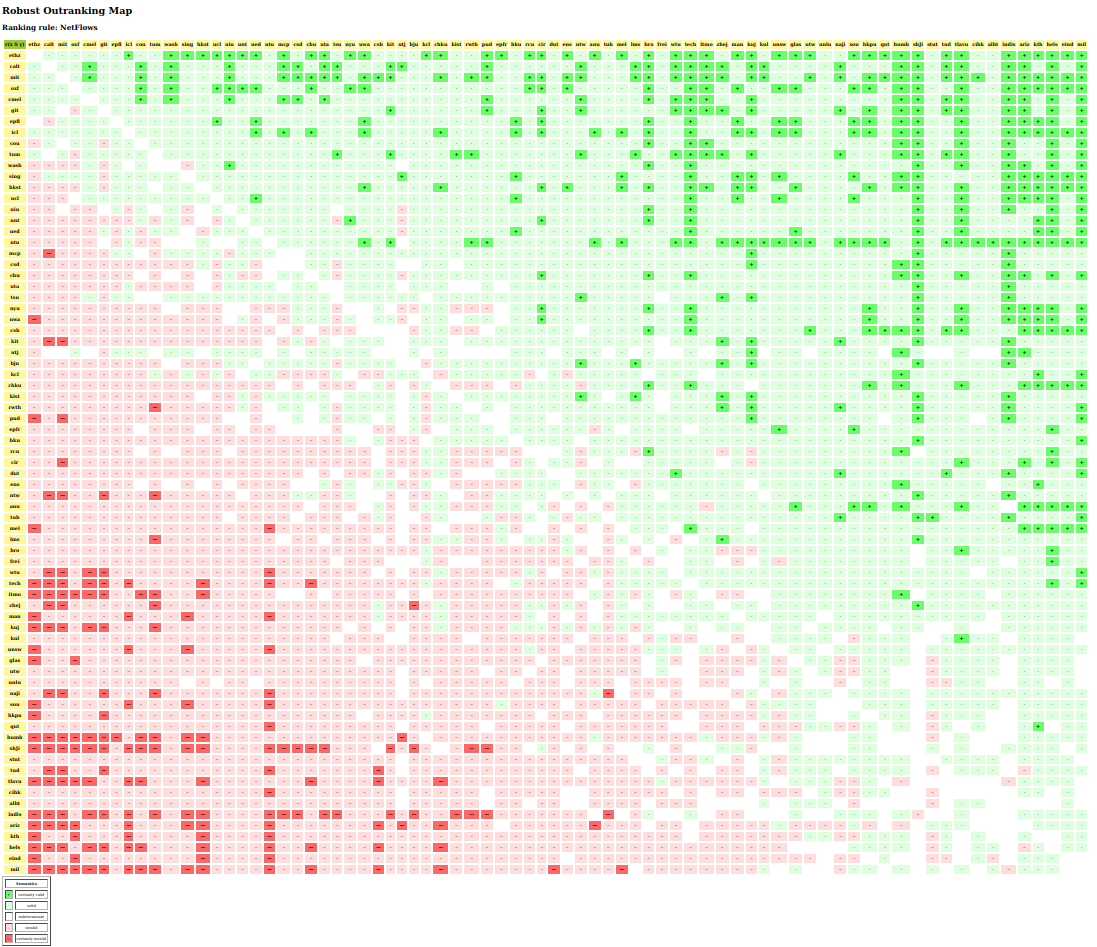
\includegraphics[width=\hsize]{Figures/13-2-the_cs_RelationMap.png}
\caption{Relation map of the robust outranking relation}
\label{fig:13.2}       % Give a unique label
\end{figure}

In Figure~\vref{fig:13.2}, \emph{dark green}, resp. \emph{light green} marked positions show certainly, resp. positively valid outranking situations, whereas \emph{dark red}, resp. \emph{light red} marked positions show certainly, respectively positively valid outranked situations. In the left upper corner one may verify that the five top-ranked Depts ([\texttt{ethz}, \texttt{calt}, \texttt{oxf}, \texttt{mit}, \texttt{cmel}]) are in fact mutually outranking each other and thus are all indifferent one to another. They give even robust \Condorcet winners by robustly outranking all other Depts.

Notice by the way that no certainly valid robust outranking (dark green) and no certainly valid robust outranked situations (dark red) appear in Figure~\vref{fig:13.3} below, resp. above the principal diagonal; none of these robust preferential situations are hence violated by the robust \NetFlows ranking. The non reflexive \emph{white} positions in the relation map, like the one between the Georgia Institute of Technology and the MIT, mark outranking or outranked situations that are not robust with respect to the given significance weight preorder. They become, hence, doubtful and are set to the indeterminate characteristic value $0.0$.

By measuring the ordinal correlation with the underlying pairwise global and marginal robust outranking situations, the quality of the robust \NetFlows ranking result can be formally evaluated with the \texttt{computeRankingCorrelation()} method\index{computeRankingCorrelation@\texttt{computeRankingCorrelation()}} and the \texttt{showCorrelation()} method\index{showCorrelation@\texttt{showCorrelation()}} (see Chap.~\ref{sec:16}).
\begin{lstlisting}[caption={Measuring the quality of the \NetFlows ranking result},label=list:13.13]
>>> corrnf = rdg.computeRankingCorrelation(nfRanking)
>>> rdg.showCorrelation(corrnf)   
  Correlation indexes:
    Crisp ordinal correlation  : +0.901
    Epistemic determination    :  0.563
    Bipolar-valued equivalence : +0.507
\end{lstlisting}

Listing~\vref{list:13.13} Line 4 indicates that the \NetFlows ranking result is indeed highly  correlated ($+0.901$, in \Kendall 's tau index sense) with the pairwise global robust outranking relation. Their bipolar-valued \emph{relational equivalence} index ($+0.51$, Line 6) indicates a more than $75\%$ criteria significance support.

With the \texttt{showRankingConsensusQuality()} method,  we can also check how the \NetFlows ranking rule is actually balancing the five ranking objectives.\index{showRankingConsensusQuality@\texttt{showRankingConsensusQua\-lity()}}
\begin{lstlisting}[caption={Measuring the consensus quality of the \NetFlows ranking result},label=list:13.14]
>>> rdg.showRankingConsensusQuality(nfRanking)
  Criterion (weight): correlation
  -------------------------------
    gtch (0.300): +0.660
    gres (0.300): +0.638
    gcit (0.275): +0.370
    gint (0.075): +0.155
    gind (0.050): +0.101
   Summary:
    Weighted mean marginal correlation (a): +0.508
    Standard deviation (b)                : +0.187
    Ranking fairness (a)-(b)              : +0.321
\end{lstlisting}

The ordinal correlation indexes with the marginal performance criterion rankings are nearly respecting the given significance weights preorder: \texttt{gtch} $\approx$ \texttt{gres} $>$ \texttt{gcit} $>$ \texttt{gint} $>$ \texttt{gind} (see Lines 4-8 above). The mean marginal ordinal correlation index is quite high ($+0.51$). Coupled with a low standard deviation ($0.187$), we obtain a quite fairly balanced ranking result (Lines 10-12). 

We can furthermore inspect with the \texttt{showCriteriaCorrelationTable()} method \index{showCriteriaCorrelationTable@\texttt{showCriteriaCorrelationTable()}} the mutual correlation indexes observed between the individual criterion based marginal robust outranking relations. 
\begin{lstlisting}[caption={Showing the ordinal correlation between the marginal criterion relations},label=list:13.15]
>>> rdg.showCriteriaCorrelationTable()
    Criteria ordinal correlation index
	 |  gcit    gind    gint    gres    gtch   
    -----|------------------------------------------
    gcit | +1.00   -0.11   +0.24   +0.13   +0.17   
    gind |         +1.00   -0.18   +0.15   +0.15   
    gint |                 +1.00   +0.04   -0.00   
    gres |                         +1.00   +0.67   
    gtch |                                 +1.00   
\end{lstlisting}

Slightly contradictory ($-0.11$) appear the \emph{Citations} and \emph{Industrial income} criteria (Line 5 Column 3 in List.~\vref{list:13.15}). Due perhaps to potential confidentiality clauses, it seams perhaps not always possible to publish industrially relevant research results in highly ranked journals. However, criteria \emph{Citations} and \emph{International outlook} show a slightly positive correlation ($+0.24$, Column 4), whereas the \emph{International outlook} criterion shows no apparent correlation with both the major \emph{Teaching} and \emph{Research} criteria. The latter are however highly correlated ($+0.67$. Line 9 Column 6).

A Principal Component Analysis may well illustrate with the \texttt{export3Dplot\-OfCriteriaCorrelation()} method the previous findings \citep{CPSTAT-L2}. \index{export3DplotOfCriteriaCorrelation@\texttt{export3DplotOfCriteria\-Correlation()}}
\begin{lstlisting}
>>> rdg.export3DplotOfCriteriaCorrelation(graphType='pdf')
\end{lstlisting}
\begin{figure}[ht]
%\sidecaption
\includegraphics[width=\hsize]{Figures/13-3-3DCorrelation.pdf}
\caption{3D PCA plot of the pairwise criteria correlation table}
\label{fig:13.3}       % Give a unique label
\end{figure}

In Figure~\vref{fig:13.3}, one may notice first that more than $80\%$ of the total variance of the previous correlation table is explained by the apparent opposition between the marginal outrankings of criteria: \emph{Teaching}, \emph{Research} and \emph{Industry income} on the left side, and the marginal outrankings of criteria: \emph{Citations} and \emph{International outlook} on the right side. Notice also in the left lower corner the nearly identical positions of the marginal outrankings of the major \emph{Teaching} and \emph{Research} criteria. In the factors 2 and 3 plot, about $30\%$ of the total variance is captured by the opposition between the marginal outrankings of the \emph{Teaching} and \emph{Research} criteria and the marginal outrankings of the \emph{Industrial income} criterion. Finally, in the factors 1 and 3 plot, nearly $15\%$ of the total variance is explained by the opposition between the marginal outrankings of the \emph{International outlook} criterion and the marginal outrankings of the \emph{Citations} criterion.

It is, finally, interesting to similarly assess the ordinal correlation between the THE average scores-based ranking and the robust outranking digraph.
\begin{lstlisting}[caption={Computing the ordinal quality of the THE ranking},label=list:13.16]
>>> # theScores = [(xScore_1,x_1), (xScore_2,x_2),... ]
>>> # is sorted in decreasing order of xscores
>>> theRanking = [item[1] for item in theScores]
>>> corrthe = rdg.computeRankingCorrelation(theRanking)
>>> rdg.showCorrelation(corrthe)
    Correlation indexes:
     Crisp ordinal correlation  : +0.907
     Epistemic determination    :  0.563
     Bipolar-valued equivalence : +0.511
>>> rdg.showRankingConsensusQuality(theRanking)
    Criterion (weight): correlation
    -------------------------------
     gtch (0.300): +0.683
     gres (0.300): +0.670
     gcit (0.275): +0.319
     gint (0.075): +0.161
     gind (0.050): +0.106
    Summary:
     Weighted mean marginal correlation (a): +0.511
     Standard deviation (b)                : +0.210
     Ranking fairness (a)-(b)              : +0.302
\end{lstlisting}

The THE ranking result is similarly correlated ($+0.907$, Line 7 in List.~\ref{list:13.16}) with the pairwise global robust outranking situations. By its overall weighted scoring rule, the THE ranking naturally induces marginal criterion correlations that are compatible with the given significance weight preorder (Lines 13-17). Notice that the mean marginal correlation is of a similar value ($+0.51$, Line 19) as the robust \NetFlows ranking. Yet, its standard deviation is slightly higher, which leads to a less fairer balancing of the three major ranking criteria.

To conclude, let us emphasise, that, without any commensurability hypothesis and by taking, furthermore, into account, first, the always present more or less imprecision of any performance evaluation and, secondly, solely ordinal criteria significance weights, we may obtain here with our robust outranking approach a very similar ranking result with a slightly better preference modelling quality. A convincing heatmap view of the 25 first-ranked Institutions may eventually be generated in the default system browser with following command.
\begin{lstlisting}
>>> rdg.showHTMLPerformanceHeatmap(
...            WithActionNames=True,\
...            outrankingModel='this',\
...            rankingRule='NetFlows',\
...            ndigits=1,\
...            Correlations=True,\
...            fromIndex=0,toIndex=25)
\end{lstlisting}
\begin{figure}[ht]
%\sidecaption
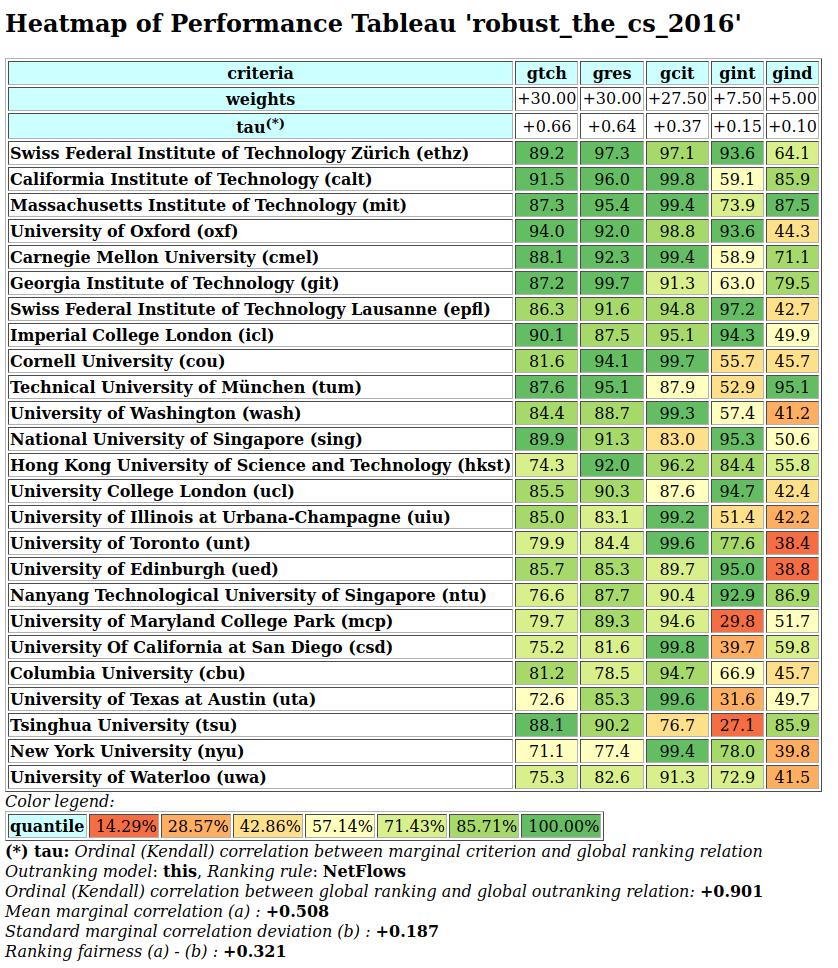
\includegraphics[width=\hsize]{Figures/13-4-theHeatmap.png}
\caption{Extract of a heatmap browser view on the \NetFlows ranking result}
\label{fig:13.4}       % Give a unique label
\end{figure}

As an exercise, the reader is invited to try out other robust outranking based ranking heuristics. Notice also that we have not challenged in this case study the THE provided criteria significance preorder. It would be very interesting to consider the five ranking objectives as equally important and, consequently, consider the ranking criteria to be equisignificant. Curious to see the ranking results under such settings.
 
%%%%%%% The chapter bibliography
%\normallatexbib
%\clearpage
\phantomsection
\addcontentsline{toc}{section}{Chapter Bibliography}
\chapter{The best academic Computer Science Depts: A ranking case study}
\label{sec:13}

\abstract*{ In this case study, we are solving with our \Digraph resources a ranking decision problem based on published data from the \emph{Times Higher Education} (THE) \emph{World University Rankings} 2016 by \emph{Computer Science} (CS) subject. Several hundred academic CS Departments, from all over the world, were ranked that year following an overall numerical score based on the weighted average of five performance criteria: \emph{Teaching} (the learning environment, $30\%$), \emph{Research} (volume, income and reputation, $30\%$), \emph{Citations} (research influence, $27.5\%$), \emph{International outlook} (staff, students, and research, $7.5\%$), and \emph{Industry income} (innovation, $5\%$). To illustrate our \Digraph programming resources, we shall first have a look into the THE ranking data with short Python scripts. In a second section, we shall relax the commensurability hypothesis of the ranking criteria and show how to similarly rank with multiple incommensurable performance criteria of solely ordinal significance. A third Section is finally devoted to introduce quality measures for qualifying ranking results.}

\abstract{ In this case study, we are solving with our \Digraph resources a ranking decision problem based on published data from the \emph{Times Higher Education} (THE) \emph{World University Rankings} 2016 by \emph{Computer Science} (CS) subject. Several hundred academic CS Departments, from all over the world, were ranked that year following an overall numerical score based on the weighted average of five performance criteria: \emph{Teaching} (the learning environment, $30\%$), \emph{Research} (volume, income and reputation, $30\%$), \emph{Citations} (research influence, $27.5\%$), \emph{International outlook} (staff, students, and research, $7.5\%$), and \emph{Industry income} (innovation, $5\%$). To illustrate our \Digraph programming resources, we shall first have a look into the THE multiple-criteria ranking data with short Python scripts. In a second section, we shall relax the commensurability hypothesis of the ranking criteria and show how to similarly rank with multiple incommensurable performance criteria of solely ordinal significance. A third section is finally devoted to introduce quality measures for qualifying ranking results.
}

\section{The THE performance tableau}
\label{sec:13.1}

For this decision making case study, we use an extract of the published \THE (THE) World University rankings 2016 by Computer Science (CS) subject, concerning the 75 first-ranked academic Institutions\footnote{\href{https://www.timeshighereducation.com/world-university-rankings/2017/subject-ranking/computer-science}{THE World University Rankings 2016 by Computer Science subject}}. The multiple-criteria performance tableau data, collected from the THE web pages, is stored in a file named \texttt{the-cs-2016.py} of \texttt{PerformanceTableau} format \footnote{The performance tableau \texttt{the-cs-2016.py} is available in the \texttt{examples} directory of the \Digraph resources \citep{BIS-2021}.}.\index{THE University rankings 2016 by CS subject} 
\begin{lstlisting}[caption={Performance tableau of the },label=list:13.1]
>>> from perfTabs import PerformanceTableau
>>> cspt = PerformanceTableau('the_cs_2016')
>>> cspt
  *------- PerformanceTableau instance description ------*
   Instance class     : PerformanceTableau
   Instance name      : the-cs-2016
   Actions            : 75
   Objectives         : 5
   Criteria           : 5
   NaN proportion (%) : 0.0
   Attributes         : ['name','description','actions',
                           'objectives','criteria',
			   'weightPreorder','NA','evaluation']
\end{lstlisting}

Potential decision alternatives, in our case here, are the 75 THE best-ranked CS Departments in 2016, all of them located at world renowned Institutions, like California Institute of Technology, Swiss Federal Institute of Technology Zurich, Technical University München, University of Oxford or the National University of Singapore (see List.~\vref{list:13.2} below). 

Instead of using prefigured \Digraph \texttt{show...()} methods, readily available for inspecting \texttt{PerformanceTableau} instances, Listing~\vref{list:13.2} illustrates how to write small Python scripts for printing out its content.   
\begin{lstlisting}[caption={Printing the CS Departments},label=list:13.2,basicstyle=\ttfamily\scriptsize]
>>> for x in cspt.actions:
...     print('%s:\t%s (%s)' %\
...        (x,cspt.actions[x]['name'],cspt.actions[x]['comment']) )
  albt:	University of Alberta (CA)
  anu:	Australian National University (AU)
  ariz:	Arizona State University (US)
  bju:	Beijing University (CN)
  bro:	Brown University (US)
  calt:	California Institute of Technology (US)
  cbu:	Columbia University (US)
  chku:	Chinese University of Hong Kong (HK)
  cihk:	City University of Hong Kong (HK)
  cir:	University of California at Irvine (US)
  cmel:	Carnegie Mellon University (US)
  cou:	Cornell University (US)
  csb:	University of California at Santa Barbara (US)
  csd:	University Of California at San Diego (US)
  dut:	Delft University of Technology (NL)
  eind:	Eindhoven University of Technology (NL)
  ens:	Superior Normal School at Paris (FR)
  epfl:	Swiss Federal Institute of Technology Lausanne (CH)
  epfr:	Polytechnic school of Paris (FR)
  ethz:	Swiss Federal Institute of Technology Zurich (CH)
  frei:	University of Freiburg (DE)
  git:	Georgia Institute of Technology (US)
  glas:	University of Glasgow (UK)
  hels:	University of Helsinki (FI)
  hkpu:	Hong Kong Polytechnic University (CN)
  hkst:	Hong Kong University of Science and Technology (HK)
  hku:	Hong Kong University (HK)
  humb:	Berlin Humboldt University (DE)
  icl:	Imperial College London (UK)
  indis:Indian Institute of Science (IN)
  itmo:	ITMO University (RU)
  kcl:	King's College London (UK)
  kist:	Korea Adv. Institute of Science and Technology (KR)
  kit:	Karlsruhe Institute of Technology (DE)
  kth:	KTH Royal Institute of Technology (SE)
  kuj:	Kyoto University (JP)
  kul:	Catholic University Leuven (BE)
  lms:	Lomonosov Moscow State University (RU)
  man:	University of Manchester (UK)
  mcp:	University of Maryland College Park (US)
  mel:	University of Melbourne (AU)
  mil:	Polytechnic University of Milan (IT)
  mit:	Massachusetts Institute of Technology (US)
  naji:	Nanjing University (CN)
  ntu:	Nanyang Technological University of Singapore (SG)
  ntw:	National Taiwan University (TW)
  nyu:	New York University (US)
  oxf:	University of Oxford (UK)
  pud:	Purdue University (US)
  qut:	Queensland University of Technology (AU)
  rcu:	Rice University (US)
  rwth:	RWTH Aachen University (DE)
  shJi:	Shanghai Jiao Tong University (CN)
  sing:	National University of Singapore (SG)
  sou:	University of Southhampton (UK)
  stut:	University of Stuttgart (DE)
  tech:	Technion - Israel Institute of Technology (IL)
  tlavu:Tel Aviv University (IR)
  tsu:	Tsinghua University (CN)
  tub:	Technical University of Berlin (DE)
  tud:	Technical University of Darmstadt (DE)
  tum:	Technical University of Muenchen (DE)
  ucl:	University College London (UK)
  ued:	University of Edinburgh (UK)
  uiu:	University of Illinois at Urbana-Champagne (US)
  unlu:	University of Luxembourg (LU)
  unsw:	University of New South Wales (AU)
  unt:	University of Toronto (CA)
  uta:	University of Texas at Austin (US)
  utj:	University of Tokyo (JP)
  utw:	University of Twente (NL)
  uwa:	University of Waterloo (CA)
  wash:	University of Washington (US)
  wtu:	Vienna University of Technology (AUS)
  zhej:	Zhejiang University (CN)
\end{lstlisting}

The THE authors base their 2016 ranking on five decision objectives \citep{THE-2016}.
\begin{lstlisting}[caption={The THE ranking objectives},label=list:13.3,basicstyle=\ttfamily\scriptsize]
>>> for obj in cspt.objectives:
...     print('%s: %s (%.1f%%),\n\t%s' %\
...                (obj,cspt.objectives[obj]['name'],\
...                 cspt.objectives[obj]['weight'],
...                 cspt.objectives[obj]['comment'])\
...           ) 
 Teaching: Best learning environment (30.0%)
   Reputation survey; Staff-to-student ration;
   Doctorate-to-student ratio;
   Doctorate-to-academic-staff ratio;
   Institutional income.
 Research: Highest volume and reputation (30.0%)
   Reputation survey;
   Research income;
   Research productivity.
 Citations: Highest research influence (27.5%)
   Impact.
 International outlook: Most international staff,
                        students and research (7.5%)
   Proportions of international students;
   Proportions of international staff;
   International collaborations.
 Industry income: Best knowledge transfer (5.0%)
   Volume.
\end{lstlisting}

With a cumulated importance of $87\%$ (see above), \emph{Teaching}, \emph{Research} and \emph{Citations} represent clearly the major ranking objectives. \emph{International outlook} and \emph{Industry income} are considered of minor importance ($12.5\%$).

THE authors do, unfortunately, not publish the detail of their performance assessments for evaluating CS Depts with respect to each one of performance criteria per ranking objective.  \footnote{THE gives some insight on the subject and significance of the actual ranking criteria used for evaluating along each ranking objective on her website \citep{THE-2016}}. The THE 2016 ranking publication reveals solely a compound assessment on a single performance criteria per ranking objective. The five retained performance criteria may be printed out as follows.
\begin{lstlisting}
>>> for g in cspt.criteria:
...     print('%s:\t%s, %s (%.1f%%)' %\
...       (g,cspt.criteria[g]['name'],cspt.criteria[g]['comment'],\
...        cspt.criteria[g]['weight']) )  
  gtch:	Teaching, The learning environment (30.0%)
  gres:	Research, Volume, income and reputation (30.0%)
  gcit:	Citations, Research influence (27.5%)
  gint:	International outlook, In staff, students and research (7.5%)
  gind:	Industry income, knowledge transfer (5.0%)
\end{lstlisting}

The largest part ($87.5\%$) of criteria significance is, hence canonically, allocated to the major ranking criteria: \emph{Teaching} ($30\%$), \emph{Research} ($30\%$) and \emph{Citations} ($27.5\%$). The small remaining part ($12.5\%$) goes to \emph{International outlook} ($7.5\%$) and \emph{Industry income} ($5\%$).

In order to render commensurable these performance criteria, the THE authors replace, per criterion, the actual performance evaluation obtained by each University with the corresponding \emph{quantile} observed in the cumulative distribution of the performance evaluations obtained by all the surveyed institutions \citep{THE-2016}. The THE ranking is eventually determined by an \emph{overall score} per University which corresponds to the weighted average of these five criteria quantiles, as illustrated in Listing~\vref{list:13.4}.     
\begin{lstlisting}[caption={Computing the THE overall scores},label=list:13.4]
>>> theScores = []
>>> for x in cspt.actions:
...     xscore = Decimal('0')
...     for g in cspt.criteria:
...         xscore += cspt.evaluation[g][x] *\
...          (cspt.criteria[g]['weight']/Decimal('100'))
...	   theScores.append((xscore,x))
\end{lstlisting}

In Listing~\vref{list:13.5} (Lines 15-16), we may thus notice that, in the 2016 edition of the THE World University rankings by CS subject, the Swiss Federal Institute of Technology Zürich is first-ranked with an overall score of $92.9$; followed by the California Institute of Technology (overall score: $92.4$) \footnote{The author's own Computer Science Dept at the University of Luxembourg was ranked on position 63 with an overall score of $58.0$.}.
\begin{lstlisting}[caption={Printing the ranked performance table},label=list:13.5,basicstyle=\ttfamily\scriptsize]
>>> theScores.sort(reverse = True)
>>> print('##  Univ \tgtch  gres  gcit  gint  gind  overall')
>>> print('-------------------------------------------------') 
>>> i = 1
>>> for it in theScores:
...     x = it[1]
...     xScore = it[0]
...     print('%2d: %s' % (i,x), end=' \t')
...     for g in cspt.criteria:
...         print('%.1f ' % (cspt.evaluation[g][x]),end=' ')
...	    print(' %.1f' % xScore)
...         i += 1   
    ##  Univ 	gtch  gres  gcit  gint  gind  overall
    -------------------------------------------------
     1: ethz 	89.2  97.3  97.1  93.6  64.1   92.9
     2: calt 	91.5  96.0  99.8  59.1  85.9   92.4
     3: oxf 	94.0  92.0  98.8  93.6  44.3   92.2
     4: mit 	87.3  95.4  99.4  73.9  87.5   92.1
     5: git 	87.2  99.7  91.3  63.0  79.5   89.9
     6: cmel 	88.1  92.3  99.4  58.9  71.1   89.4
     7: icl 	90.1  87.5  95.1  94.3  49.9   89.0
     8: epfl 	86.3  91.6  94.8  97.2  42.7   88.9
     9: tum 	87.6  95.1  87.9  52.9  95.1   87.7
    10: sing 	89.9  91.3  83.0  95.3  50.6   86.9
    11: cou 	81.6  94.1  99.7  55.7  45.7   86.6
    12: ucl 	85.5  90.3  87.6  94.7  42.4   86.1
    13: wash 	84.4  88.7  99.3  57.4  41.2   85.6
    14: hkst 	74.3  92.0  96.2  84.4  55.8   85.5
    15: ntu 	76.6  87.7  90.4  92.9  86.9   85.5
    16: ued 	85.7  85.3  89.7  95.0  38.8   85.0
    17: unt 	79.9  84.4  99.6  77.6  38.4   84.4
    18: uiu 	85.0  83.1  99.2  51.4  42.2   83.7
    19: mcp 	79.7  89.3  94.6  29.8  51.7   81.5
    20: cbu 	81.2  78.5  94.7  66.9  45.7   81.3
    21: tsu 	88.1  90.2  76.7  27.1  85.9   80.9
    22: csd 	75.2  81.6  99.8  39.7  59.8   80.5
    23: uwa 	75.3  82.6  91.3  72.9  41.5   80.0
    24: nyu 	71.1  77.4  99.4  78.0  39.8   79.7
    25: uta 	72.6  85.3  99.6  31.6  49.7   79.6
    26: kit 	73.8  85.5  84.4  41.3  76.8   77.9
    27: bju 	83.0  85.3  70.1  30.7  99.4   77.0
    28: csb 	65.6  70.9  94.8  72.9  74.9   76.2
    29: rwth 	77.8  85.0  70.8  43.7  89.4   76.1
    30: hku 	77.0  73.0  77.0  96.8  39.5   75.4
    31: pud 	76.9  84.8  70.8  58.1  56.7   75.2
    32: kist 	79.4  88.2  64.2  31.6  92.8   74.9
    33: kcl 	45.5  94.6  86.3  95.1  38.3   74.8
    34: chku 	64.1  69.3  94.7  75.6  49.9   74.2
    35: epfr 	81.7  60.6  78.1  85.3  62.9   73.7
    36: dut 	64.1  78.3  76.3  69.8  90.1   73.4
    37: tub 	66.2  82.4  71.0  55.4  99.9   73.3
    38: utj 	92.0  91.7  48.7  25.8  49.6   72.9
    39: cir 	68.8  64.6  93.0  65.1  40.4   72.5
    40: ntw 	81.5  79.8  66.6  25.5  67.6   72.0
    41: anu 	47.2  73.0  92.2  90.0  48.1   70.6
    42: rcu 	64.1  53.8  99.4  63.7  46.1   69.8
    43: mel 	56.1  70.2  83.7  83.3  50.4   69.7
    44: lms 	81.5  68.1  61.0  31.1  87.8   68.4
    45: ens 	71.8  40.9  98.7  69.6  43.5   68.3
    46: wtu 	61.8  73.5  73.7  51.9  62.2   67.9
    47: tech 	54.9  71.0  85.1  51.7  40.1   67.1
    48: bro 	58.5  54.9  96.8  52.3  38.6   66.5
    49: man 	63.5  71.9  62.9  84.1  42.1   66.3
    50: zhej 	73.5  70.4  60.7  22.6  75.7   65.3
    51: frei 	54.2  51.6  89.5  49.7  99.9   65.1
    52: unsw 	60.2  58.2  70.5  87.0  44.3   63.6
    53: kuj 	75.4  72.8  49.5  28.3  51.4   62.8
    54: sou 	48.2  60.7  75.5  87.4  43.2   62.1
    55: shJi 	66.9  68.3  62.4  22.8  38.5   61.4
    56: itmo 	58.0  32.0  98.7  39.2  68.7   60.5
    57: kul 	35.2  55.8  92.0  46.0  88.3   60.5
    58: glas 	35.2  52.5  91.2  85.8  39.2   59.8
    59: utw 	38.2  52.8  87.0  69.0  60.0   59.4
    60: stut 	54.2  60.6  61.1  36.3  97.8   58.9
    61: naji 	51.4  76.9  48.8  39.7  74.4   58.6
    62: tud 	46.6  53.6  75.9  53.7  66.5   58.3
    63: unlu 	35.2  44.2  87.4  99.7  54.1   58.0
    64: qut 	45.5  42.6  82.8  75.2  63.0   58.0
    65: hkpu 	46.8  36.5  91.4  73.2  41.5   57.7
    66: albt 	39.2  53.3  69.9  91.9  75.4   57.6
    67: mil 	46.4  64.3  69.2  44.1  38.5   57.5
    68: hels 	48.8  49.6  80.4  50.6  39.5   57.4
    69: cihk 	42.4  44.9  80.1  76.2  67.9   57.3
    70: tlavu 	34.1  57.2  89.0  45.3  38.6   57.2
    71: indis 	56.9  76.1  49.3  20.1  41.5   57.0
    72: ariz 	28.4  61.8  84.3  59.3  42.0   56.8
    73: kth 	44.8  42.0  83.6  71.6  39.2   56.4
    74: humb 	48.4  31.3  94.7  41.5  45.5   55.3
    75: eind 	32.4  48.4  81.5  72.2  45.8   54.4
\end{lstlisting}

It is important to notice that a ranking by weighted average scores requires \emph{commensurable ranking criteria} of precise decimal significance and on wich precise decimal performance evaluations are given. It is very unlikely that the THE 2016 performance assessments verify indeed these conditions. Here we show how to relax these methodological requirements --precise commensurable criteria and decimal evaluations-- by following instead a bipolar-valued epistemic logic based ranking methodology (see Chap.~\ref{sec:8}).

\section{Ranking with multiple criteria of ordinal significance}
\label{sec:13.2}

Let us, first, have a critical look in Figure~\vref{fig:13.1} at the THE performance criteria.
\begin{lstlisting}
>>> cspt.showHTMLCriteria(Sorted=False)
\end{lstlisting}
\begin{figure}[ht]
%\sidecaption
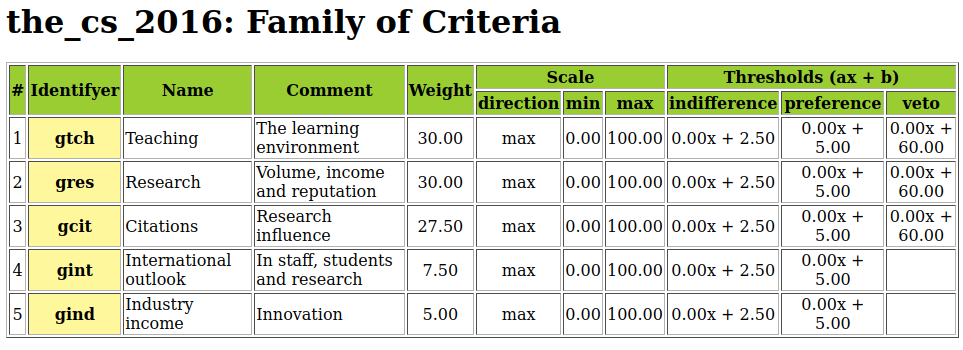
\includegraphics[width=\hsize]{Figures/13-1-the_cs_2016Criteria.png}
\caption{The THE ranking criteria}
\label{fig:13.1}       % Give a unique label
\end{figure}

Considering a very likely imprecision of the performance evaluation procedure, followed by some potential violation of uniform distributed quantile classes, we assume here that a performance quantile difference of up to $2.5\%$ is \emph{insignificant}, whereas a difference of $5\%$ and more warrants a \emph{clearly better}, resp. \emph{clearly less good} performance. With quantiles $94\%$, resp. $87.3\%$, Oxford's CS teaching environment, for instance, is thus clearly better evaluated than that of the MIT (see List.~\vref{list:13.5} Lines 27-28). We shall furthermore assume that a \emph{considerable} performance quantile difference of $60\%$, observed on the three major ranking criteria: \emph{Teaching}, \emph{Research} and \emph{Citations}, will trigger the polarisation of pairwise outranking, respectively outranked situations \citep{BIS-2013}.

The effect these performance discrimination thresholds induce on the outranking modelling can be inspected with the \texttt{showCriteria()} method\index{showCriteria@\texttt{showCriteria()}}.
\begin{lstlisting}[caption={Inspecting the performance discrimination thresholds},label=list:13.6]
>>> cspt.showCriteria()
  *----  criteria -----*
    gtch 'Teaching'
      Scale = (Decimal('0.00'), Decimal('100.00'))
      Weight = 0.300 
      Threshold ind : 2.50 + 0.00x ;   percentile:  8.07
      Threshold pref : 5.00 + 0.00x ;  percentile: 15.75
      Threshold veto : 60.00 + 0.00x ; percentile: 99.75
    gres 'Research'
      Scale = (Decimal('0.00'), Decimal('100.00'))
      Weight = 0.300 
      Threshold ind : 2.50 + 0.00x ;   percentile:  7.86
      Threshold pref : 5.00 + 0.00x ;  percentile: 16.14
      Threshold veto : 60.00 + 0.00x ; percentile: 99.21
    gcit 'Citations'
      Scale = (Decimal('0.00'), Decimal('100.00'))
      Weight = 0.275 
      Threshold ind : 2.50 + 0.00x ;   percentile:  11.82
      Threshold pref : 5.00 + 0.00x ;  percentile:  22.99
      Threshold veto : 60.00 + 0.00x ; percentile: 100.00
    gint 'International outlook'
      Scale = (Decimal('0.00'), Decimal('100.00'))
      Weight = 0.075 
      Threshold ind : 2.50 + 0.00x ;  percentile:  6.45
      Threshold pref : 5.00 + 0.00x ; percentile: 11.75
    gind 'Industry income'
      Scale = (Decimal('0.00'), Decimal('100.00'))
      Weight = 0.050 
      Threshold ind : 2.50 + 0.00x ;  percentile: 11.82
      Threshold pref : 5.00 + 0.00x ; percentile: 21.51
\end{lstlisting}

Between $6\%$ and $12\%$ of the observed quantile differences are, hence, considered to be \emph{insignificant}. Similarly, between $77\%$ and $88\%$ are considered to be \emph{significant}. Less than $1\%$ correspond to \emph{considerable} quantile differences on both the \emph{Teaching} and \emph{Research} criteria; actually triggering an epistemic polarisation effect \citep{BIS-2013}.

Beside the likely imprecise performance discrimination, the \emph{precise decimal significance weights}, as allocated by the THE authors to the five ranking criteria are, as well, quite \emph{questionable}. Criteria significance weights may carry sometimes hidden strategies for rendering the performance evaluations commensurable in view of a numerical computation of the overall ranking scores. The eventual ranking result is, the case given, as much depending on the precise values of the given criteria significance weights as, vice versa, the given precise significance weights are depending on the subjectively expected and accepted ranking results \footnote{In a social choice context, this potential double bind between voting profiles and election result, corresponds to voting manipulation strategies.}. We will therefore drop these precise decimal weights and, instead, only require a corresponding criteria significance preorder: \texttt{gtch} $=$ \texttt{gres} $>$ \texttt{gcit} $>$ \texttt{gint} $>$ \texttt{gind}. \emph{Teaching environment} and \emph{Research volume and reputation} are equally considered most significant, followed by \emph{Research influence}. Then comes \emph{International outlook in staff, students and research} and, least significant finally, \emph{Industry income and innovation}.

Both these working hypotheses: --performance discrimination thresholds and --solely ordinal criteria significance, give us way to a ranking methodology based on \emph{robust pairwise outranking} situations (see Chap.~\ref{sec:19} and \citep{BIS-2004b}).
\begin{definition}[Robust outranking situations with ordinal criteria significance weights]\label{def:13.1}
\begin{itemize}[topsep=1pt]
\item We say that CS Dept $x$ \emph{robustly outranks} CS Dept $y$ when $x$ positively outranks $y$ with \textbf{all} significance weight vectors that are compatible with the significance preorder: \texttt{gtch} $=$ \texttt{gres} $>$ \texttt{gcit} $>$ \texttt{gint} $>$ \texttt{gind};
\item We say that CS Dept $x$ is \emph{robustly outranked} by CS Dept $y$ when $x$ is positively outranked by $y$ with \textbf{all} significance weight vectors that are compatible with the significance preorder: \texttt{gtch} $=$ \texttt{gres} $>$ \texttt{gcit} $>$ \texttt{gint} $>$ \texttt{gind};
\item Otherwise, CS Depts $x$ and $y$ are considered to be \emph{incomparable}.
\end{itemize}
\end{definition}

A corresponding digraph constructor is provided by the \texttt{RobustOutranking\-Digraph} class\index{RobustOutrankingDigraph@\texttt{RobustOutrankingDigraph} class}.
\begin{lstlisting}[caption={Computing the robust outranking digraph},label=list:13.7]
>>> from outrankingDigraphs import RobustOutrankingDigraph	     
>>> rdg = RobustOutrankingDigraph(cspt)
>>> rdg
  *------- Object instance description ------*
   Instance class       : RobustOutrankingDigraph
   Instance name        : robust_the_cs_2016
   Actions              : 75
   Criteria             : 5
   Size                 : 2993
   Determinateness (%)  : 78.16
   Valuation domain     : [-1.00;1.00]
>>> rdg.computeIncomparabilityDegree(Comments=True)
  Incomparability degree (%) of digraph <robust_the_cs_2016>:
   links x<->y y: 2775, incomparable: 102, comparable: 2673
   (incomparable/links) =  0.037
>>> rdg.computeTransitivityDegree(Comments=True)
  Transitivity degree of digraph <robust_the_cs_2016>:
   triples x>y>z: 405150, closed: 218489, open: 186661
   (closed/triples) =  0.539
>>> rdg.computeSymmetryDegree(Comments=True)
  Symmetry degree (%) of digraph <robust_the_cs_2016>:
   arcs x>y: 2673, symmetric: 320, asymmetric: 2353
   (symmetric/arcs) =  0.12
\end{lstlisting}

In the resulting digraph instance \texttt{rdg} (see Line 9 in Listing~\vref{list:13.7}), we observe $2993$ such robust pairwise outranking situations validated with a mean significance of $78\%$ (Line 10). Unfortunately, in the case here, they do not deliver any complete linear ranking. The robust outranking digraph \texttt{rdg} contains 102 incomparability situations ($3.7\%$, Line 15); nearly half of its transitive closure is missing ($46.1\%$, Line 19) and $12\%$ of the positive outranking situations correspond in fact to symmetric indifference situations (Line 23).

Worse even, the digraph \texttt{rdg} admits a really high number of outranking circuits \footnote{The \texttt{computeChordlessCircuits()} and \texttt{showChordlessCircuits()} methods are separate because there are various methods available for enumerating the chordless circuits in a digraph \citep{BIS-2010}.}.\index{showChordlessCircuits@\texttt{showChordlessCircuits()}}
\begin{lstlisting}[caption={Inspecting outranking circuits},label=list:13.8]
>>> rdg.computeChordlessCircuits()
>>> rdg.showChordlessCircuits()
 *---- Chordless circuits ----*
  145 circuits.
  1:  ['albt','unlu','ariz','hels'], cred. : 0.300
  2:  ['albt','tlavu','hels'], cred. : 0.150
  3:  ['anu', 'man', 'itmo'], cred. : 0.250
  4:  ['anu', 'zhej', 'rcu'], cred. : 0.250
    ...
    ...
  82:  ['csb','epfr','rwth'], cred. : 0.250
  83:  ['csb','epfr','pud','nyu'], cred. : 0.250
  84:  ['csd','kcl','kist'], cred. : 0.250
    ...
    ...
  142:  ['kul','qut','mil'], cred. : 0.250
  143:  ['lms','rcu','tech'], cred. : 0.300
  144:  ['mil','stut','qut'], cred. : 0.300
  145:  ['mil','stut','tud'], cred. : 0.300
\end{lstlisting}

Among the 145 detected robust outranking circuits reported in Listing \vref{list:13.8}, we notice, for instance, two outranking circuits of length 4 (see circuits 1 and 83).

Let us inspect below the bipolar-valued robust outranking characteristics of the first circuit.
\begin{lstlisting}[caption={Showing the relation table with stability denotation},label=list:13.9]
>>> rdg.showRelationTable(actionsSubset=\
...         ['albt','unlu','ariz','hels'],\
...         Sorted=False) 
  * ---- Relation Table -----
   r/(stab)|  'albt' 'unlu' 'ariz' 'hels'   
      -----|-----------------------------
    'albt' |  +1.00  +0.30  +0.00  +0.00  
           |   (+4)   (+2)   (-1)   (-1)  
    'unlu' |  +0.00  +1.00  +0.40  +0.00  
           |   (+0)   (+4)   (+2)   (-1)  
    'ariz' |  +0.00  -0.12  +1.00  +0.40  
           |   (+1)   (-2)   (+4)   (+2)  
    'hels' |  +0.45  +0.00  -0.03  +1.00  
           |   (+2)   (+1)   (-2)   (+4)  
   Valuation domain: [-1.0; 1.0]
   Stability denotation semantics:
   +4|-4 : unanimous outranking | outranked situation;
   +2|-2 : outranking | outranked situation validated
      with all potential significance weights that are
      compatible with the given significance preorder;
   +1|-1 : validated outranking | outranked situation
      with the given significance weights;
     0   : indeterminate relational situation.
\end{lstlisting}

In Listing~\vref{list:13.9}, we notice that the robust outranking circuit \texttt{[albt,} \texttt{unlu,} \texttt{ariz,} \texttt{hels]}  will reappear with all potential criteria significance weight vectors that are compatible with given preorder: \texttt{gtch} $=$ \texttt{gres} $>$ \texttt{gcit} $>$ \texttt{gint} $>$ \texttt{gind}. Notice also the ($\pm 1$) marked outranking situations, like the one between \texttt{albt} and \texttt{ariz}. The statement that ``\emph{Arizona State University strictly  outranks University of Alberta}'' is in fact valid with the precise THE criteria significance weights, but not with all potential significance weights vectors that are compatible with the given significance preorder. All these ($\pm 1$)  marked outranking situations become hence \emph{doubtful} ($r(x \succsim y) = 0.00$) and the corresponding CS Depts, like University of Alberta and Arizona State University, become \emph{incomparable} in a robust outranking sense.  

Showing many incomparabilities and indifferences; not being transitive and containing many robust outranking circuits; all these relational characteristics, make that no ranking algorithm, applied to digraph \texttt{rdg}, does exist that would produce a \emph{unique} optimal linear ranking result. Methodologically, we are only left with ranking heuristics. In Chapter~\ref{sec:8} on ranking with multiple criteria we have now seen several potential heuristic ranking rules that can be used for ranking with an outranking digraph; yet, they may deliver potentially more or less diverging results. Considering the order of digraph \texttt{rdg} (75) and the largely unequal THE criteria significance weights, we rather opt, in this tutorial, for the \NetFlows ranking rule \footnote{The reader might try other ranking rules, like the \Copeland or \Kohler rules. Mind that the latter ranking-by-choosing rule is more complex (see Chap.~\ref{sec:8}).}. Its complexity in $O(n^2)$ is indeed quite tractable and, by avoiding potential \emph{tyranny of short majority} effects, the \NetFlows rule may specifically take the ranking criteria significance weights into a more fairly balanced account.

The \NetFlows ranking result of the CS Depts can be directly computed with the \texttt{computeNetFlowsRanking()} method\index{computeNetFlowsRanking@\texttt{computeNetFlowsRanking()}}. 
\begin{lstlisting}[caption={Computing a robust \NetFlows ranking},label=list:13.10]
>>> nfRanking = rdg.computeNetFlowsRanking()
>>> nfRanking
  ['ethz','calt','mit', 'oxf',  'cmel','git', 'epfl',
   'icl', 'cou', 'tum', 'wash', 'sing','hkst','ucl',
   'uiu', 'unt', 'ued', 'ntu',  'mcp', 'csd', 'cbu',
   'uta', 'tsu', 'nyu', 'uwa',  'csb', 'kit', 'utj',
   'bju', 'kcl', 'chku','kist', 'rwth','pud', 'epfr',
   'hku', 'rcu', 'cir', 'dut',  'ens', 'ntw', 'anu',
   'tub', 'mel', 'lms', 'bro',  'frei','wtu', 'tech',
   'itmo','zhej','man', 'kuj',  'kul', 'unsw','glas',
   'utw', 'unlu','naji','sou',  'hkpu','qut', 'humb',
   'shJi','stut','tud', 'tlavu','cihk','albt','indis',
   'ariz','kth', 'hels','eind', 'mil']
\end{lstlisting}

We actually obtain in Listing~\vref{list:13.10} a very similar ranking result as the one obtained with the THE average scores. The same group of seven Depts: \texttt{ethz}, \texttt{calt}, \texttt{mit}, \texttt{oxf}, \texttt{cmel}, \texttt{git} and \texttt{epfl}, is top-ranked. And a same group of Depts: \texttt{tlavu}, \texttt{cihk}, \texttt{indis}, \texttt{ariz}, \texttt{kth}, \texttt{hels}, \texttt{eind}, and \texttt{mil} appears at the end of the list.

We can print out the difference between the overall scores based THE ranking and the \NetFlows ranking above with the following short Python script, where we make use of an ordered Python dictionary with net-flow scores, stored in the \texttt{rdg.netFlowsRankingDict} attribute by the previous computation.
\begin{lstlisting}[caption={Comparing the robust \NetFlows ranking with the THE ranking},label=list:13.11,basicstyle=\ttfamily\scriptsize]
>>> # rdg.netFlowsRankingDict: ordered dictionary with net flow
>>> # scores stored in rdg by the computeNetFlowsRanking() method
>>> # theScores = [(xScore_1,x_1), (xScore_2,x_2),... ]
>>> # is sorted in decreasing order of xscores_i
>>> print(\
...  ' NetFlows ranking   gtch  gres  gcit  gint  gind   THE ranking')
>>> for i in range(75):
...     x = nfRanking[i]
...     xScore = rdg.netFlowsRankingDict[x]['netFlow']
...     thexScore,thex = theScores[i]
...     print('%2d: %s (%.2f) ' % (i+1,x,xScore), end=' \t')
...     for g in rdg.criteria:
...         print('%.1f ' % (t.evaluation[g][x]),end=' ')
...     print(' %s (%.2f)' % (thex,thexScore) )  
  NetFlows ranking   gtch  gres  gcit  gint  gind   THE ranking
   1: ethz (116.95)  89.2  97.3  97.1  93.6  64.1   ethz (92.88)
   2: calt (116.15)  91.5  96.0  99.8  59.1  85.9   calt (92.42)
   3: mit (112.72)   87.3  95.4  99.4  73.9  87.5   oxf (92.20)
   4: oxf (112.00)   94.0  92.0  98.8  93.6  44.3   mit (92.06)
   5: cmel (101.60)  88.1  92.3  99.4  58.9  71.1   git (89.88)
   6: git (93.40)    87.2  99.7  91.3  63.0  79.5   cmel (89.43)
   7: epfl (90.88)   86.3  91.6  94.8  97.2  42.7   icl (89.00)
   8: icl (90.62)    90.1  87.5  95.1  94.3  49.9   epfl (88.86)
   9: cou (84.60)    81.6  94.1  99.7  55.7  45.7   tum (87.70)
  10: tum (80.42)    87.6  95.1  87.9  52.9  95.1   sing (86.86)
  11: wash (76.28)   84.4  88.7  99.3  57.4  41.2   cou (86.59)
  12: sing (73.05)   89.9  91.3  83.0  95.3  50.6   ucl (86.05)
  13: hkst (71.05)   74.3  92.0  96.2  84.4  55.8   wash (85.60)
  14: ucl (66.78)    85.5  90.3  87.6  94.7  42.4   hkst (85.47)
  15: uiu (64.80)    85.0  83.1  99.2  51.4  42.2   ntu (85.46)
  16: unt (62.65)    79.9  84.4  99.6  77.6  38.4   ued (85.03)
  17: ued (58.67)    85.7  85.3  89.7  95.0  38.8   unt (84.42)
  18: ntu (57.88)    76.6  87.7  90.4  92.9  86.9   uiu (83.67)
  19: mcp (54.08)    79.7  89.3  94.6  29.8  51.7   mcp (81.53)
  20: csd (46.62)    75.2  81.6  99.8  39.7  59.8   cbu (81.25)
  21: cbu (44.27)    81.2  78.5  94.7  66.9  45.7   tsu (80.91)
  22: uta (43.27)    72.6  85.3  99.6  31.6  49.7   csd (80.45)
  23: tsu (42.42)    88.1  90.2  76.7  27.1  85.9   uwa (80.02)
  24: nyu (35.30)    71.1  77.4  99.4  78.0  39.8   nyu (79.72)
  25: uwa (28.88)    75.3  82.6  91.3  72.9  41.5   uta (79.61)
  26: csb (18.18)    65.6  70.9  94.8  72.9  74.9   kit (77.94)
  27: kit (16.32)    73.8  85.5  84.4  41.3  76.8   bju (77.04)
  28: utj (15.95)    92.0  91.7  48.7  25.8  49.6   csb (76.23)
  29: bju (15.45)    83.0  85.3  70.1  30.7  99.4   rwth (76.06)
  30: kcl (11.95)    45.5  94.6  86.3  95.1  38.3   hku (75.41)
  31: chku (9.43)    64.1  69.3  94.7  75.6  49.9   pud (75.17)
  32: kist (7.30)    79.4  88.2  64.2  31.6  92.8   kist (74.94)
  33: rwth (5.00)    77.8  85.0  70.8  43.7  89.4   kcl (74.81)
  34: pud (2.40)     76.9  84.8  70.8  58.1  56.7   chku (74.23)
  35: epfr (-1.70)   81.7  60.6  78.1  85.3  62.9   epfr (73.71)
  36: hku (-3.83)    77.0  73.0  77.0  96.8  39.5   dut (73.44)
  37: rcu (-6.38)    64.1  53.8  99.4  63.7  46.1   tub (73.25)
  38: cir (-8.20)    68.8  64.6  93.0  65.1  40.4   utj (72.92)
  39: dut (-8.85)    64.1  78.3  76.3  69.8  90.1   cir (72.50)
  40: ens (-8.97)    71.8  40.9  98.7  69.6  43.5   ntw (72.00)
  41: ntw (-11.15)   81.5  79.8  66.6  25.5  67.6   anu (70.57)
  42: anu (-11.50)   47.2  73.0  92.2  90.0  48.1   rcu (69.79)
  43: tub (-12.20)   66.2  82.4  71.0  55.4  99.9   mel (69.67)
  44: mel (-23.98)   56.1  70.2  83.7  83.3  50.4   lms (68.38)
  45: lms (-25.43)   81.5  68.1  61.0  31.1  87.8   ens (68.35)
  46: bro (-27.18)   58.5  54.9  96.8  52.3  38.6   wtu (67.86)
  47: frei (-34.42)  54.2  51.6  89.5  49.7  99.9   tech (67.06)
  48: wtu (-35.05)   61.8  73.5  73.7  51.9  62.2   bro (66.49)
  49: tech (-37.95)  54.9  71.0  85.1  51.7  40.1   man (66.33)
  50: itmo (-38.50)  58.0  32.0  98.7  39.2  68.7   zhej (65.34)
  51: zhej (-43.70)  73.5  70.4  60.7  22.6  75.7   frei (65.08)
  52: man (-44.83)   63.5  71.9  62.9  84.1  42.1   unsw (63.65)
  53: kuj (-47.40)   75.4  72.8  49.5  28.3  51.4   kuj (62.77)
  54: kul (-49.98)   35.2  55.8  92.0  46.0  88.3   sou (62.15)
  55: unsw (-54.88)  60.2  58.2  70.5  87.0  44.3   shJi (61.35)
  56: glas (-56.98)  35.2  52.5  91.2  85.8  39.2   itmo (60.52)
  57: utw (-59.27)   38.2  52.8  87.0  69.0  60.0   kul (60.47)
  58: unlu (-60.08)  35.2  44.2  87.4  99.7  54.1   glas (59.78)
  59: naji (-60.52)  51.4  76.9  48.8  39.7  74.4   utw (59.40)
  60: sou (-60.83)   48.2  60.7  75.5  87.4  43.2   stut (58.85)
  61: hkpu (-62.05)  46.8  36.5  91.4  73.2  41.5   naji (58.61)
  62: qut (-66.17)   45.5  42.6  82.8  75.2  63.0   tud (58.28)
  63: humb (-68.10)  48.4  31.3  94.7  41.5  45.5   unlu (58.04)
  64: shJi (-69.72)  66.9  68.3  62.4  22.8  38.5   qut (57.99)
  65: stut (-69.90)  54.2  60.6  61.1  36.3  97.8   hkpu (57.69)
  66: tud (-70.83)   46.6  53.6  75.9  53.7  66.5   albt (57.63)
  67: tlavu (-71.50) 34.1  57.2  89.0  45.3  38.6   mil (57.47)
  68: cihk (-72.20)  42.4  44.9  80.1  76.2  67.9   hels (57.40)
  69: albt (-72.33)  39.2  53.3  69.9  91.9  75.4   cihk (57.33)
  70: indis (-72.53) 56.9  76.1  49.3  20.1  41.5   tlavu (57.19)
  71: ariz (-75.10)  28.4  61.8  84.3  59.3  42.0   indis (57.04)
  72: kth (-77.10)   44.8  42.0  83.6  71.6  39.2   ariz (56.79)
  73: hels (-79.55)  48.8  49.6  80.4  50.6  39.5   kth (56.36)
  74: eind (-82.85)  32.4  48.4  81.5  72.2  45.8   humb (55.34)
  75: mil (-83.67)   46.4  64.3  69.2  44.1  38.5   eind (54.36)
\end{lstlisting}

The first inversion we observe in Listing~\vref{list:13.11} (Lines 18-19) concerns Oxford University and the MIT, switching positions 3 and 4. Most inversions are similarly short and concern only switching very close positions in either way. There are some slightly more important inversions concerning, for instance, the Hong Kong University CS Dept, ranked into position 30 in the THE ranking and here in the position 36 (Line 51). The opposite situation may also happen; the Berlin Humboldt University CS Dept, occupying the 74th position in the THE ranking, advances in the robust \NetFlows ranking to position 63 (Line 78).

In our bipolar-valued epistemic framework, the \NetFlows score of any CS Dept $x$ corresponds to the criteria significance support for the logical statement ``$x$ \emph{is first-ranked}''. Formally 
\begin{equation}\label{eq:13.1}
  r(x \; \text{is first-ranked}) \; = \; \sum_{y \neq x} r\big((x \succsim y) \,+\, (y \not\succsim x)\big) \;=\; \sum_{y \neq x} \big(r(x \succsim y) - r(y \succsim x)\big).
\end{equation}

Using the robust outranking characteristics of digraph \texttt{rdg}, we can thus explicitly compute, for instance, ETH Zürich's \NetFlows score, denoted \texttt{nfx} below.
\begin{lstlisting}
>>> x = 'ethz'
>>> nfx = Decimal('0')
>>> for y in rdg.actions:
...     if x != y:
...         nfx += (rdg.relation[x][y]\
...                - rdg.relation[y][x])  
>>> print(x, nfx)
  ethz 116.950
\end{lstlisting}

In Listing~\vref{list:13.11} (Line 16), one may now verify that ETH Zürich obtains indeed the highest \NetFlows score $116.95$, and gives, hence the \emph{most credible} first-ranked CS Dept of the 75 potential candidates.

Yet, how may we now convince the reader, that the outranking based ranking result here appears more objective and trustworthy, than the classic value theory based THE ranking by average quantile scores?  

\section{How to judge the quality of a ranking result?}
\label{sec:13.3}

In a multiple-criteria based ranking problem, inspecting pairwise marginal performance differences may give objectivity to global preferential statements. That a CS Dept $x$ convincingly outranks Dept $y$ can conveniently be checked with the \texttt{showPairwiseOutrankings()} method.\index{showPairwiseOutrankings@\texttt{showPairwiseOutrankings()}}. The ETH Zürich CS Dept is, for instance, first ranked before Caltech's Dept in both previous rankings. Lest us check the preferential reasons.
\begin{lstlisting}[caption={Comparing pairwise criteria performances},label=list:13.12,basicstyle=\ttfamily\scriptsize]
>>> rdg.showPairwiseOutrankings('ethz','calt')
  *------------  pairwise comparisons ----*
  Valuation in range: -100.00 to +100.00
  Comparing actions : ('ethz', 'calt')
  crit.    wght.  g(ethz)  g(calt) diff  | ind  pref     r()  | 
  --------------------------------------   -------------------
  'gcit'   27.50   97.10   99.80   -2.70 | 2.50  5.00   +0.00 | 
  'gind'    5.00   64.10   85.90  -21.80 | 2.50  5.00   -5.00 | 
  'gint'    7.50   93.60   59.10  +34.50 | 2.50  5.00   +7.50 | 
  'gres'   30.00   97.30   96.00   +1.30 | 2.50  5.00  +30.00 | 
  'gtch'   30.00   89.20   91.50   -2.30 | 2.50  5.00  +30.00 |
                                                     ------
                                         r(x >= y):  +62.50
  crit.    wght.  g(calt)  g(ethz) diff  | ind   pref    r()  |
  ---------------------------------------   -----------------
  'gcit'   27.50   99.80   97.10   +2.70 | 2.50  5.00  +27.50 | 
  'gind'    5.00   85.90   64.10  +21.80 | 2.50  5.00   +5.00 | 
  'gint'    7.50   59.10   93.60  -34.50 | 2.50  5.00   -7.50 | 
  'gres'   30.00   96.00   97.30   -1.30 | 2.50  5.00  +30.00 | 
  'gtch'   30.00   91.50   89.20   +2.30 | 2.50  5.00  +30.00 |
                                                      -------
                                            r(y >= x): +85.00
\end{lstlisting}

A significant positive performance difference ($+34.50$), concerning the \emph{International outlook} criterion (of $7,5\%$ significance), is observed in Listing~\vref{list:13.12} in favour of the ETH Zürich Dept (Line 9 above). Similarly, a significant positive performance difference ($+21.80$), concerning the \emph{Industry income} criterion (of $5\%$ significance), is observed, this time, in favour of the Caltech Dept (Line 17). The former, larger positive, performance difference, observed on a more significant criterion, gives so far a first convincing argument of $12.5\%$ significance for putting ETH Zürich first, before Caltech. Yet, the slightly positive performance difference ($+2.70$, Line 16) between Caltech and ETH Zürich on the \emph{Citations} criterion (of $27.5\%$ significance) confirms an ``\emph{at least as well evaluated as}'' situation in favour of the Caltech Dept.

The inverse negative performance difference ($-2.70$, Line 7), however, is neither \emph{significant} ($< -5.00$), nor \emph{insignificant} ($> -2.50$), and does hence neither confirm nor infirm a ``\emph{not at least as well evaluated as}'' situation in disfavour of ETH Zürich. We observe here a convincing argument of $27.5\%$ significance for ranking Caltech first, before ETH Zürich.

Notice finally, that, on the \emph{Teaching} and \emph{Research} criteria of total significance $60\%$, both Depts do, with performance differences $(< \mid 2.50 \mid)$, perform one as well as the other. As these two major performance criteria together necessarily admit always the highest significance with the imposed significance weight preorder: \texttt{gtch} $=$ \texttt{gres} $>$ \texttt{gcit} $>$ \texttt{gint} $>$ \texttt{gind}, both outranking situations get in fact globally confirmed at stability level $+2$ (see Chap.~\ref{sec:19}).

A browser view of the corresponding robust relation map, ordering the CS Depts again with the same \NetFlows ranking rule, well illustrates all such \emph{stable outranking} situations.
\begin{lstlisting}
>>> rdg.showHTMLRelationMap(\
...            tableTitle='Robust Outranking Map',
...            rankingRule='NetFlows')
\end{lstlisting}
\begin{figure}[ht]
%\sidecaption
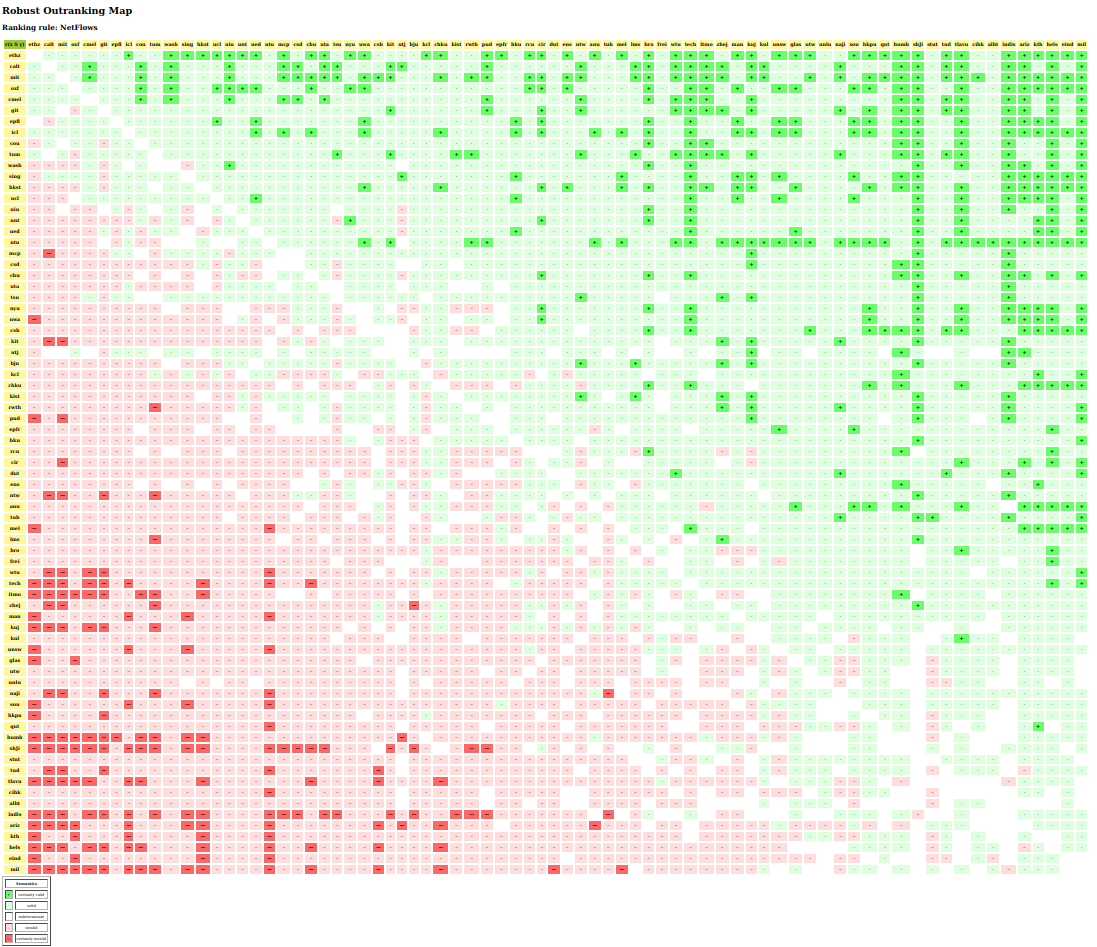
\includegraphics[width=\hsize]{Figures/13-2-the_cs_RelationMap.png}
\caption{Relation map of the robust outranking relation}
\label{fig:13.2}       % Give a unique label
\end{figure}

In Figure~\vref{fig:13.2}, \emph{dark green}, resp. \emph{light green} marked positions show certainly, resp. positively valid outranking situations, whereas \emph{dark red}, resp. \emph{light red} marked positions show certainly, respectively positively valid outranked situations. In the left upper corner one may verify that the five top-ranked Depts ([\texttt{ethz}, \texttt{calt}, \texttt{oxf}, \texttt{mit}, \texttt{cmel}]) are in fact mutually outranking each other and thus are all indifferent one to another. They give even robust \Condorcet winners by robustly outranking all other Depts.

Notice by the way that no certainly valid robust outranking (dark green) and no certainly valid robust outranked situations (dark red) appear in Figure~\vref{fig:13.3} below, resp. above the principal diagonal; none of these robust preferential situations are hence violated by the robust \NetFlows ranking. The non reflexive \emph{white} positions in the relation map, like the one between the Georgia Institute of Technology and the MIT, mark outranking or outranked situations that are not robust with respect to the given significance weight preorder. They become, hence, doubtful and are set to the indeterminate characteristic value $0.0$.

By measuring the ordinal correlation with the underlying pairwise global and marginal robust outranking situations, the quality of the robust \NetFlows ranking result can be formally evaluated with the \texttt{computeRankingCorrelation()} method\index{computeRankingCorrelation@\texttt{computeRankingCorrelation()}} and the \texttt{showCorrelation()} method\index{showCorrelation@\texttt{showCorrelation()}} (see Chap.~\ref{sec:16}).
\begin{lstlisting}[caption={Measuring the quality of the \NetFlows ranking result},label=list:13.13]
>>> corrnf = rdg.computeRankingCorrelation(nfRanking)
>>> rdg.showCorrelation(corrnf)   
  Correlation indexes:
    Crisp ordinal correlation  : +0.901
    Epistemic determination    :  0.563
    Bipolar-valued equivalence : +0.507
\end{lstlisting}

Listing~\vref{list:13.13} Line 4 indicates that the \NetFlows ranking result is indeed highly  correlated ($+0.901$, in \Kendall 's tau index sense) with the pairwise global robust outranking relation. Their bipolar-valued \emph{relational equivalence} index ($+0.51$, Line 6) indicates a more than $75\%$ criteria significance support.

With the \texttt{showRankingConsensusQuality()} method,  we can also check how the \NetFlows ranking rule is actually balancing the five ranking objectives.\index{showRankingConsensusQuality@\texttt{showRankingConsensusQua\-lity()}}
\begin{lstlisting}[caption={Measuring the consensus quality of the \NetFlows ranking result},label=list:13.14]
>>> rdg.showRankingConsensusQuality(nfRanking)
  Criterion (weight): correlation
  -------------------------------
    gtch (0.300): +0.660
    gres (0.300): +0.638
    gcit (0.275): +0.370
    gint (0.075): +0.155
    gind (0.050): +0.101
   Summary:
    Weighted mean marginal correlation (a): +0.508
    Standard deviation (b)                : +0.187
    Ranking fairness (a)-(b)              : +0.321
\end{lstlisting}

The ordinal correlation indexes with the marginal performance criterion rankings are nearly respecting the given significance weights preorder: \texttt{gtch} $\approx$ \texttt{gres} $>$ \texttt{gcit} $>$ \texttt{gint} $>$ \texttt{gind} (see Lines 4-8 above). The mean marginal ordinal correlation index is quite high ($+0.51$). Coupled with a low standard deviation ($0.187$), we obtain a quite fairly balanced ranking result (Lines 10-12). 

We can furthermore inspect with the \texttt{showCriteriaCorrelationTable()} method \index{showCriteriaCorrelationTable@\texttt{showCriteriaCorrelationTable()}} the mutual correlation indexes observed between the individual criterion based marginal robust outranking relations. 
\begin{lstlisting}[caption={Showing the ordinal correlation between the marginal criterion relations},label=list:13.15]
>>> rdg.showCriteriaCorrelationTable()
    Criteria ordinal correlation index
	 |  gcit    gind    gint    gres    gtch   
    -----|------------------------------------------
    gcit | +1.00   -0.11   +0.24   +0.13   +0.17   
    gind |         +1.00   -0.18   +0.15   +0.15   
    gint |                 +1.00   +0.04   -0.00   
    gres |                         +1.00   +0.67   
    gtch |                                 +1.00   
\end{lstlisting}

Slightly contradictory ($-0.11$) appear the \emph{Citations} and \emph{Industrial income} criteria (Line 5 Column 3 in List.~\vref{list:13.15}). Due perhaps to potential confidentiality clauses, it seams perhaps not always possible to publish industrially relevant research results in highly ranked journals. However, criteria \emph{Citations} and \emph{International outlook} show a slightly positive correlation ($+0.24$, Column 4), whereas the \emph{International outlook} criterion shows no apparent correlation with both the major \emph{Teaching} and \emph{Research} criteria. The latter are however highly correlated ($+0.67$. Line 9 Column 6).

A Principal Component Analysis may well illustrate with the \texttt{export3Dplot\-OfCriteriaCorrelation()} method the previous findings \citep{CPSTAT-L2}. \index{export3DplotOfCriteriaCorrelation@\texttt{export3DplotOfCriteria\-Correlation()}}
\begin{lstlisting}
>>> rdg.export3DplotOfCriteriaCorrelation(graphType='pdf')
\end{lstlisting}
\begin{figure}[ht]
%\sidecaption
\includegraphics[width=\hsize]{Figures/13-3-3DCorrelation.pdf}
\caption{3D PCA plot of the pairwise criteria correlation table}
\label{fig:13.3}       % Give a unique label
\end{figure}

In Figure~\vref{fig:13.3}, one may notice first that more than $80\%$ of the total variance of the previous correlation table is explained by the apparent opposition between the marginal outrankings of criteria: \emph{Teaching}, \emph{Research} and \emph{Industry income} on the left side, and the marginal outrankings of criteria: \emph{Citations} and \emph{International outlook} on the right side. Notice also in the left lower corner the nearly identical positions of the marginal outrankings of the major \emph{Teaching} and \emph{Research} criteria. In the factors 2 and 3 plot, about $30\%$ of the total variance is captured by the opposition between the marginal outrankings of the \emph{Teaching} and \emph{Research} criteria and the marginal outrankings of the \emph{Industrial income} criterion. Finally, in the factors 1 and 3 plot, nearly $15\%$ of the total variance is explained by the opposition between the marginal outrankings of the \emph{International outlook} criterion and the marginal outrankings of the \emph{Citations} criterion.

It is, finally, interesting to similarly assess the ordinal correlation between the THE average scores-based ranking and the robust outranking digraph.
\begin{lstlisting}[caption={Computing the ordinal quality of the THE ranking},label=list:13.16]
>>> # theScores = [(xScore_1,x_1), (xScore_2,x_2),... ]
>>> # is sorted in decreasing order of xscores
>>> theRanking = [item[1] for item in theScores]
>>> corrthe = rdg.computeRankingCorrelation(theRanking)
>>> rdg.showCorrelation(corrthe)
    Correlation indexes:
     Crisp ordinal correlation  : +0.907
     Epistemic determination    :  0.563
     Bipolar-valued equivalence : +0.511
>>> rdg.showRankingConsensusQuality(theRanking)
    Criterion (weight): correlation
    -------------------------------
     gtch (0.300): +0.683
     gres (0.300): +0.670
     gcit (0.275): +0.319
     gint (0.075): +0.161
     gind (0.050): +0.106
    Summary:
     Weighted mean marginal correlation (a): +0.511
     Standard deviation (b)                : +0.210
     Ranking fairness (a)-(b)              : +0.302
\end{lstlisting}

The THE ranking result is similarly correlated ($+0.907$, Line 7 in List.~\ref{list:13.16}) with the pairwise global robust outranking situations. By its overall weighted scoring rule, the THE ranking naturally induces marginal criterion correlations that are compatible with the given significance weight preorder (Lines 13-17). Notice that the mean marginal correlation is of a similar value ($+0.51$, Line 19) as the robust \NetFlows ranking. Yet, its standard deviation is slightly higher, which leads to a less fairer balancing of the three major ranking criteria.

To conclude, let us emphasise, that, without any commensurability hypothesis and by taking, furthermore, into account, first, the always present more or less imprecision of any performance evaluation and, secondly, solely ordinal criteria significance weights, we may obtain here with our robust outranking approach a very similar ranking result with a slightly better preference modelling quality. A convincing heatmap view of the 25 first-ranked Institutions may eventually be generated in the default system browser with following command.
\begin{lstlisting}
>>> rdg.showHTMLPerformanceHeatmap(
...            WithActionNames=True,\
...            outrankingModel='this',\
...            rankingRule='NetFlows',\
...            ndigits=1,\
...            Correlations=True,\
...            fromIndex=0,toIndex=25)
\end{lstlisting}
\begin{figure}[ht]
%\sidecaption
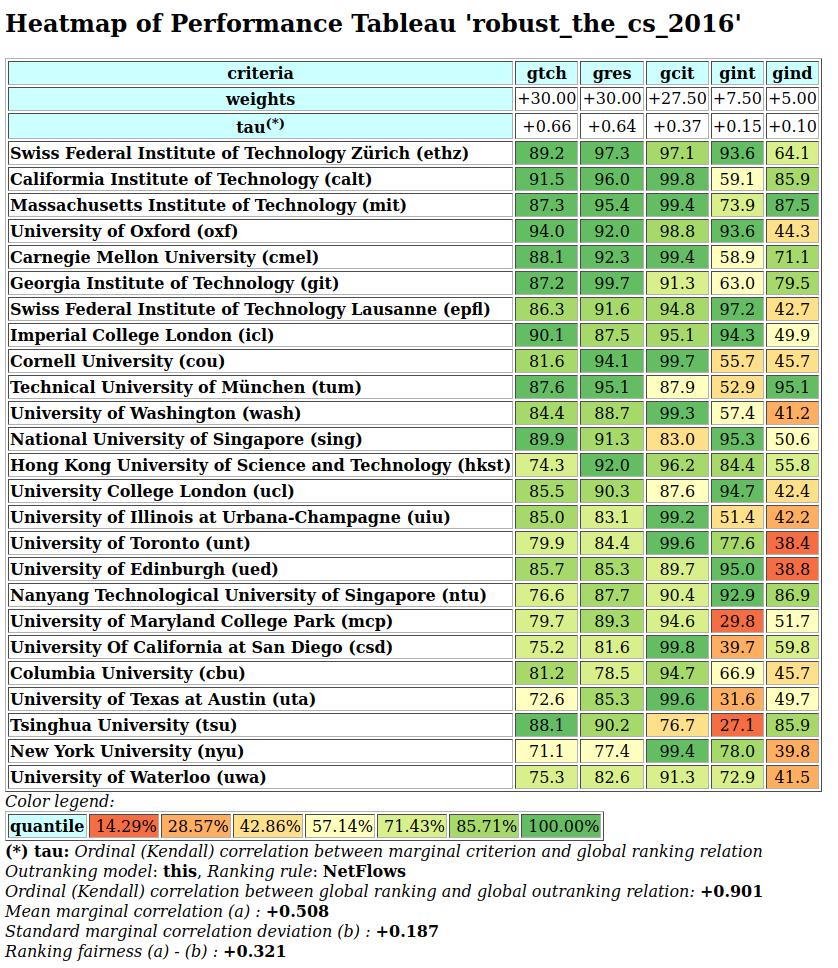
\includegraphics[width=\hsize]{Figures/13-4-theHeatmap.png}
\caption{Extract of a heatmap browser view on the \NetFlows ranking result}
\label{fig:13.4}       % Give a unique label
\end{figure}

As an exercise, the reader is invited to try out other robust outranking based ranking heuristics. Notice also that we have not challenged in this case study the THE provided criteria significance preorder. It would be very interesting to consider the five ranking objectives as equally important and, consequently, consider the ranking criteria to be equisignificant. Curious to see the ranking results under such settings.
 
%%%%%%% The chapter bibliography
%\normallatexbib
%\clearpage
\phantomsection
\addcontentsline{toc}{section}{Chapter Bibliography}
\chapter{The best academic Computer Science Depts: A ranking case study}
\label{sec:13}

\abstract*{ In this case study, we are solving with our \Digraph resources a ranking decision problem based on published data from the \emph{Times Higher Education} (THE) \emph{World University Rankings} 2016 by \emph{Computer Science} (CS) subject. Several hundred academic CS Departments, from all over the world, were ranked that year following an overall numerical score based on the weighted average of five performance criteria: \emph{Teaching} (the learning environment, $30\%$), \emph{Research} (volume, income and reputation, $30\%$), \emph{Citations} (research influence, $27.5\%$), \emph{International outlook} (staff, students, and research, $7.5\%$), and \emph{Industry income} (innovation, $5\%$). To illustrate our \Digraph programming resources, we shall first have a look into the THE ranking data with short Python scripts. In a second section, we shall relax the commensurability hypothesis of the ranking criteria and show how to similarly rank with multiple incommensurable performance criteria of solely ordinal significance. A third Section is finally devoted to introduce quality measures for qualifying ranking results.}

\abstract{ In this case study, we are solving with our \Digraph resources a ranking decision problem based on published data from the \emph{Times Higher Education} (THE) \emph{World University Rankings} 2016 by \emph{Computer Science} (CS) subject. Several hundred academic CS Departments, from all over the world, were ranked that year following an overall numerical score based on the weighted average of five performance criteria: \emph{Teaching} (the learning environment, $30\%$), \emph{Research} (volume, income and reputation, $30\%$), \emph{Citations} (research influence, $27.5\%$), \emph{International outlook} (staff, students, and research, $7.5\%$), and \emph{Industry income} (innovation, $5\%$). To illustrate our \Digraph programming resources, we shall first have a look into the THE multiple-criteria ranking data with short Python scripts. In a second section, we shall relax the commensurability hypothesis of the ranking criteria and show how to similarly rank with multiple incommensurable performance criteria of solely ordinal significance. A third section is finally devoted to introduce quality measures for qualifying ranking results.
}

\section{The THE performance tableau}
\label{sec:13.1}

For this decision making case study, we use an extract of the published \THE (THE) World University rankings 2016 by Computer Science (CS) subject, concerning the 75 first-ranked academic Institutions\footnote{\href{https://www.timeshighereducation.com/world-university-rankings/2017/subject-ranking/computer-science}{THE World University Rankings 2016 by Computer Science subject}}. The multiple-criteria performance tableau data, collected from the THE web pages, is stored in a file named \texttt{the-cs-2016.py} of \texttt{PerformanceTableau} format \footnote{The performance tableau \texttt{the-cs-2016.py} is available in the \texttt{examples} directory of the \Digraph resources \citep{BIS-2021}.}.\index{THE University rankings 2016 by CS subject} 
\begin{lstlisting}[caption={Performance tableau of the },label=list:13.1]
>>> from perfTabs import PerformanceTableau
>>> cspt = PerformanceTableau('the_cs_2016')
>>> cspt
  *------- PerformanceTableau instance description ------*
   Instance class     : PerformanceTableau
   Instance name      : the-cs-2016
   Actions            : 75
   Objectives         : 5
   Criteria           : 5
   NaN proportion (%) : 0.0
   Attributes         : ['name','description','actions',
                           'objectives','criteria',
			   'weightPreorder','NA','evaluation']
\end{lstlisting}

Potential decision alternatives, in our case here, are the 75 THE best-ranked CS Departments in 2016, all of them located at world renowned Institutions, like California Institute of Technology, Swiss Federal Institute of Technology Zurich, Technical University München, University of Oxford or the National University of Singapore (see List.~\vref{list:13.2} below). 

Instead of using prefigured \Digraph \texttt{show...()} methods, readily available for inspecting \texttt{PerformanceTableau} instances, Listing~\vref{list:13.2} illustrates how to write small Python scripts for printing out its content.   
\begin{lstlisting}[caption={Printing the CS Departments},label=list:13.2,basicstyle=\ttfamily\scriptsize]
>>> for x in cspt.actions:
...     print('%s:\t%s (%s)' %\
...        (x,cspt.actions[x]['name'],cspt.actions[x]['comment']) )
  albt:	University of Alberta (CA)
  anu:	Australian National University (AU)
  ariz:	Arizona State University (US)
  bju:	Beijing University (CN)
  bro:	Brown University (US)
  calt:	California Institute of Technology (US)
  cbu:	Columbia University (US)
  chku:	Chinese University of Hong Kong (HK)
  cihk:	City University of Hong Kong (HK)
  cir:	University of California at Irvine (US)
  cmel:	Carnegie Mellon University (US)
  cou:	Cornell University (US)
  csb:	University of California at Santa Barbara (US)
  csd:	University Of California at San Diego (US)
  dut:	Delft University of Technology (NL)
  eind:	Eindhoven University of Technology (NL)
  ens:	Superior Normal School at Paris (FR)
  epfl:	Swiss Federal Institute of Technology Lausanne (CH)
  epfr:	Polytechnic school of Paris (FR)
  ethz:	Swiss Federal Institute of Technology Zurich (CH)
  frei:	University of Freiburg (DE)
  git:	Georgia Institute of Technology (US)
  glas:	University of Glasgow (UK)
  hels:	University of Helsinki (FI)
  hkpu:	Hong Kong Polytechnic University (CN)
  hkst:	Hong Kong University of Science and Technology (HK)
  hku:	Hong Kong University (HK)
  humb:	Berlin Humboldt University (DE)
  icl:	Imperial College London (UK)
  indis:Indian Institute of Science (IN)
  itmo:	ITMO University (RU)
  kcl:	King's College London (UK)
  kist:	Korea Adv. Institute of Science and Technology (KR)
  kit:	Karlsruhe Institute of Technology (DE)
  kth:	KTH Royal Institute of Technology (SE)
  kuj:	Kyoto University (JP)
  kul:	Catholic University Leuven (BE)
  lms:	Lomonosov Moscow State University (RU)
  man:	University of Manchester (UK)
  mcp:	University of Maryland College Park (US)
  mel:	University of Melbourne (AU)
  mil:	Polytechnic University of Milan (IT)
  mit:	Massachusetts Institute of Technology (US)
  naji:	Nanjing University (CN)
  ntu:	Nanyang Technological University of Singapore (SG)
  ntw:	National Taiwan University (TW)
  nyu:	New York University (US)
  oxf:	University of Oxford (UK)
  pud:	Purdue University (US)
  qut:	Queensland University of Technology (AU)
  rcu:	Rice University (US)
  rwth:	RWTH Aachen University (DE)
  shJi:	Shanghai Jiao Tong University (CN)
  sing:	National University of Singapore (SG)
  sou:	University of Southhampton (UK)
  stut:	University of Stuttgart (DE)
  tech:	Technion - Israel Institute of Technology (IL)
  tlavu:Tel Aviv University (IR)
  tsu:	Tsinghua University (CN)
  tub:	Technical University of Berlin (DE)
  tud:	Technical University of Darmstadt (DE)
  tum:	Technical University of Muenchen (DE)
  ucl:	University College London (UK)
  ued:	University of Edinburgh (UK)
  uiu:	University of Illinois at Urbana-Champagne (US)
  unlu:	University of Luxembourg (LU)
  unsw:	University of New South Wales (AU)
  unt:	University of Toronto (CA)
  uta:	University of Texas at Austin (US)
  utj:	University of Tokyo (JP)
  utw:	University of Twente (NL)
  uwa:	University of Waterloo (CA)
  wash:	University of Washington (US)
  wtu:	Vienna University of Technology (AUS)
  zhej:	Zhejiang University (CN)
\end{lstlisting}

The THE authors base their 2016 ranking on five decision objectives \citep{THE-2016}.
\begin{lstlisting}[caption={The THE ranking objectives},label=list:13.3,basicstyle=\ttfamily\scriptsize]
>>> for obj in cspt.objectives:
...     print('%s: %s (%.1f%%),\n\t%s' %\
...                (obj,cspt.objectives[obj]['name'],\
...                 cspt.objectives[obj]['weight'],
...                 cspt.objectives[obj]['comment'])\
...           ) 
 Teaching: Best learning environment (30.0%)
   Reputation survey; Staff-to-student ration;
   Doctorate-to-student ratio;
   Doctorate-to-academic-staff ratio;
   Institutional income.
 Research: Highest volume and reputation (30.0%)
   Reputation survey;
   Research income;
   Research productivity.
 Citations: Highest research influence (27.5%)
   Impact.
 International outlook: Most international staff,
                        students and research (7.5%)
   Proportions of international students;
   Proportions of international staff;
   International collaborations.
 Industry income: Best knowledge transfer (5.0%)
   Volume.
\end{lstlisting}

With a cumulated importance of $87\%$ (see above), \emph{Teaching}, \emph{Research} and \emph{Citations} represent clearly the major ranking objectives. \emph{International outlook} and \emph{Industry income} are considered of minor importance ($12.5\%$).

THE authors do, unfortunately, not publish the detail of their performance assessments for evaluating CS Depts with respect to each one of performance criteria per ranking objective.  \footnote{THE gives some insight on the subject and significance of the actual ranking criteria used for evaluating along each ranking objective on her website \citep{THE-2016}}. The THE 2016 ranking publication reveals solely a compound assessment on a single performance criteria per ranking objective. The five retained performance criteria may be printed out as follows.
\begin{lstlisting}
>>> for g in cspt.criteria:
...     print('%s:\t%s, %s (%.1f%%)' %\
...       (g,cspt.criteria[g]['name'],cspt.criteria[g]['comment'],\
...        cspt.criteria[g]['weight']) )  
  gtch:	Teaching, The learning environment (30.0%)
  gres:	Research, Volume, income and reputation (30.0%)
  gcit:	Citations, Research influence (27.5%)
  gint:	International outlook, In staff, students and research (7.5%)
  gind:	Industry income, knowledge transfer (5.0%)
\end{lstlisting}

The largest part ($87.5\%$) of criteria significance is, hence canonically, allocated to the major ranking criteria: \emph{Teaching} ($30\%$), \emph{Research} ($30\%$) and \emph{Citations} ($27.5\%$). The small remaining part ($12.5\%$) goes to \emph{International outlook} ($7.5\%$) and \emph{Industry income} ($5\%$).

In order to render commensurable these performance criteria, the THE authors replace, per criterion, the actual performance evaluation obtained by each University with the corresponding \emph{quantile} observed in the cumulative distribution of the performance evaluations obtained by all the surveyed institutions \citep{THE-2016}. The THE ranking is eventually determined by an \emph{overall score} per University which corresponds to the weighted average of these five criteria quantiles, as illustrated in Listing~\vref{list:13.4}.     
\begin{lstlisting}[caption={Computing the THE overall scores},label=list:13.4]
>>> theScores = []
>>> for x in cspt.actions:
...     xscore = Decimal('0')
...     for g in cspt.criteria:
...         xscore += cspt.evaluation[g][x] *\
...          (cspt.criteria[g]['weight']/Decimal('100'))
...	   theScores.append((xscore,x))
\end{lstlisting}

In Listing~\vref{list:13.5} (Lines 15-16), we may thus notice that, in the 2016 edition of the THE World University rankings by CS subject, the Swiss Federal Institute of Technology Zürich is first-ranked with an overall score of $92.9$; followed by the California Institute of Technology (overall score: $92.4$) \footnote{The author's own Computer Science Dept at the University of Luxembourg was ranked on position 63 with an overall score of $58.0$.}.
\begin{lstlisting}[caption={Printing the ranked performance table},label=list:13.5,basicstyle=\ttfamily\scriptsize]
>>> theScores.sort(reverse = True)
>>> print('##  Univ \tgtch  gres  gcit  gint  gind  overall')
>>> print('-------------------------------------------------') 
>>> i = 1
>>> for it in theScores:
...     x = it[1]
...     xScore = it[0]
...     print('%2d: %s' % (i,x), end=' \t')
...     for g in cspt.criteria:
...         print('%.1f ' % (cspt.evaluation[g][x]),end=' ')
...	    print(' %.1f' % xScore)
...         i += 1   
    ##  Univ 	gtch  gres  gcit  gint  gind  overall
    -------------------------------------------------
     1: ethz 	89.2  97.3  97.1  93.6  64.1   92.9
     2: calt 	91.5  96.0  99.8  59.1  85.9   92.4
     3: oxf 	94.0  92.0  98.8  93.6  44.3   92.2
     4: mit 	87.3  95.4  99.4  73.9  87.5   92.1
     5: git 	87.2  99.7  91.3  63.0  79.5   89.9
     6: cmel 	88.1  92.3  99.4  58.9  71.1   89.4
     7: icl 	90.1  87.5  95.1  94.3  49.9   89.0
     8: epfl 	86.3  91.6  94.8  97.2  42.7   88.9
     9: tum 	87.6  95.1  87.9  52.9  95.1   87.7
    10: sing 	89.9  91.3  83.0  95.3  50.6   86.9
    11: cou 	81.6  94.1  99.7  55.7  45.7   86.6
    12: ucl 	85.5  90.3  87.6  94.7  42.4   86.1
    13: wash 	84.4  88.7  99.3  57.4  41.2   85.6
    14: hkst 	74.3  92.0  96.2  84.4  55.8   85.5
    15: ntu 	76.6  87.7  90.4  92.9  86.9   85.5
    16: ued 	85.7  85.3  89.7  95.0  38.8   85.0
    17: unt 	79.9  84.4  99.6  77.6  38.4   84.4
    18: uiu 	85.0  83.1  99.2  51.4  42.2   83.7
    19: mcp 	79.7  89.3  94.6  29.8  51.7   81.5
    20: cbu 	81.2  78.5  94.7  66.9  45.7   81.3
    21: tsu 	88.1  90.2  76.7  27.1  85.9   80.9
    22: csd 	75.2  81.6  99.8  39.7  59.8   80.5
    23: uwa 	75.3  82.6  91.3  72.9  41.5   80.0
    24: nyu 	71.1  77.4  99.4  78.0  39.8   79.7
    25: uta 	72.6  85.3  99.6  31.6  49.7   79.6
    26: kit 	73.8  85.5  84.4  41.3  76.8   77.9
    27: bju 	83.0  85.3  70.1  30.7  99.4   77.0
    28: csb 	65.6  70.9  94.8  72.9  74.9   76.2
    29: rwth 	77.8  85.0  70.8  43.7  89.4   76.1
    30: hku 	77.0  73.0  77.0  96.8  39.5   75.4
    31: pud 	76.9  84.8  70.8  58.1  56.7   75.2
    32: kist 	79.4  88.2  64.2  31.6  92.8   74.9
    33: kcl 	45.5  94.6  86.3  95.1  38.3   74.8
    34: chku 	64.1  69.3  94.7  75.6  49.9   74.2
    35: epfr 	81.7  60.6  78.1  85.3  62.9   73.7
    36: dut 	64.1  78.3  76.3  69.8  90.1   73.4
    37: tub 	66.2  82.4  71.0  55.4  99.9   73.3
    38: utj 	92.0  91.7  48.7  25.8  49.6   72.9
    39: cir 	68.8  64.6  93.0  65.1  40.4   72.5
    40: ntw 	81.5  79.8  66.6  25.5  67.6   72.0
    41: anu 	47.2  73.0  92.2  90.0  48.1   70.6
    42: rcu 	64.1  53.8  99.4  63.7  46.1   69.8
    43: mel 	56.1  70.2  83.7  83.3  50.4   69.7
    44: lms 	81.5  68.1  61.0  31.1  87.8   68.4
    45: ens 	71.8  40.9  98.7  69.6  43.5   68.3
    46: wtu 	61.8  73.5  73.7  51.9  62.2   67.9
    47: tech 	54.9  71.0  85.1  51.7  40.1   67.1
    48: bro 	58.5  54.9  96.8  52.3  38.6   66.5
    49: man 	63.5  71.9  62.9  84.1  42.1   66.3
    50: zhej 	73.5  70.4  60.7  22.6  75.7   65.3
    51: frei 	54.2  51.6  89.5  49.7  99.9   65.1
    52: unsw 	60.2  58.2  70.5  87.0  44.3   63.6
    53: kuj 	75.4  72.8  49.5  28.3  51.4   62.8
    54: sou 	48.2  60.7  75.5  87.4  43.2   62.1
    55: shJi 	66.9  68.3  62.4  22.8  38.5   61.4
    56: itmo 	58.0  32.0  98.7  39.2  68.7   60.5
    57: kul 	35.2  55.8  92.0  46.0  88.3   60.5
    58: glas 	35.2  52.5  91.2  85.8  39.2   59.8
    59: utw 	38.2  52.8  87.0  69.0  60.0   59.4
    60: stut 	54.2  60.6  61.1  36.3  97.8   58.9
    61: naji 	51.4  76.9  48.8  39.7  74.4   58.6
    62: tud 	46.6  53.6  75.9  53.7  66.5   58.3
    63: unlu 	35.2  44.2  87.4  99.7  54.1   58.0
    64: qut 	45.5  42.6  82.8  75.2  63.0   58.0
    65: hkpu 	46.8  36.5  91.4  73.2  41.5   57.7
    66: albt 	39.2  53.3  69.9  91.9  75.4   57.6
    67: mil 	46.4  64.3  69.2  44.1  38.5   57.5
    68: hels 	48.8  49.6  80.4  50.6  39.5   57.4
    69: cihk 	42.4  44.9  80.1  76.2  67.9   57.3
    70: tlavu 	34.1  57.2  89.0  45.3  38.6   57.2
    71: indis 	56.9  76.1  49.3  20.1  41.5   57.0
    72: ariz 	28.4  61.8  84.3  59.3  42.0   56.8
    73: kth 	44.8  42.0  83.6  71.6  39.2   56.4
    74: humb 	48.4  31.3  94.7  41.5  45.5   55.3
    75: eind 	32.4  48.4  81.5  72.2  45.8   54.4
\end{lstlisting}

It is important to notice that a ranking by weighted average scores requires \emph{commensurable ranking criteria} of precise decimal significance and on wich precise decimal performance evaluations are given. It is very unlikely that the THE 2016 performance assessments verify indeed these conditions. Here we show how to relax these methodological requirements --precise commensurable criteria and decimal evaluations-- by following instead a bipolar-valued epistemic logic based ranking methodology (see Chap.~\ref{sec:8}).

\section{Ranking with multiple criteria of ordinal significance}
\label{sec:13.2}

Let us, first, have a critical look in Figure~\vref{fig:13.1} at the THE performance criteria.
\begin{lstlisting}
>>> cspt.showHTMLCriteria(Sorted=False)
\end{lstlisting}
\begin{figure}[ht]
%\sidecaption
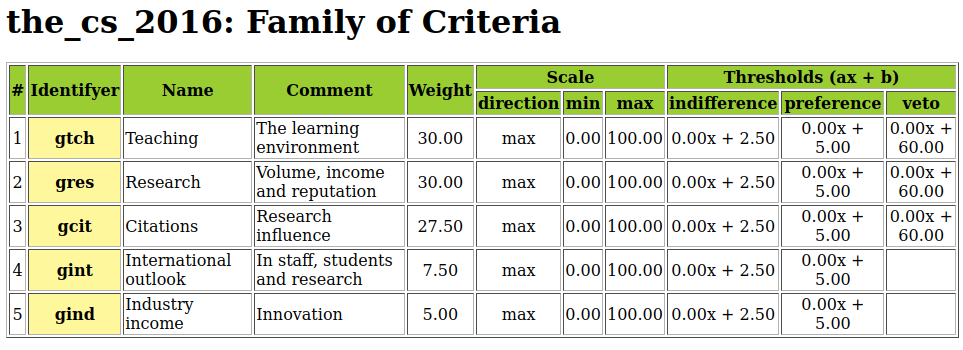
\includegraphics[width=\hsize]{Figures/13-1-the_cs_2016Criteria.png}
\caption{The THE ranking criteria}
\label{fig:13.1}       % Give a unique label
\end{figure}

Considering a very likely imprecision of the performance evaluation procedure, followed by some potential violation of uniform distributed quantile classes, we assume here that a performance quantile difference of up to $2.5\%$ is \emph{insignificant}, whereas a difference of $5\%$ and more warrants a \emph{clearly better}, resp. \emph{clearly less good} performance. With quantiles $94\%$, resp. $87.3\%$, Oxford's CS teaching environment, for instance, is thus clearly better evaluated than that of the MIT (see List.~\vref{list:13.5} Lines 27-28). We shall furthermore assume that a \emph{considerable} performance quantile difference of $60\%$, observed on the three major ranking criteria: \emph{Teaching}, \emph{Research} and \emph{Citations}, will trigger the polarisation of pairwise outranking, respectively outranked situations \citep{BIS-2013}.

The effect these performance discrimination thresholds induce on the outranking modelling can be inspected with the \texttt{showCriteria()} method\index{showCriteria@\texttt{showCriteria()}}.
\begin{lstlisting}[caption={Inspecting the performance discrimination thresholds},label=list:13.6]
>>> cspt.showCriteria()
  *----  criteria -----*
    gtch 'Teaching'
      Scale = (Decimal('0.00'), Decimal('100.00'))
      Weight = 0.300 
      Threshold ind : 2.50 + 0.00x ;   percentile:  8.07
      Threshold pref : 5.00 + 0.00x ;  percentile: 15.75
      Threshold veto : 60.00 + 0.00x ; percentile: 99.75
    gres 'Research'
      Scale = (Decimal('0.00'), Decimal('100.00'))
      Weight = 0.300 
      Threshold ind : 2.50 + 0.00x ;   percentile:  7.86
      Threshold pref : 5.00 + 0.00x ;  percentile: 16.14
      Threshold veto : 60.00 + 0.00x ; percentile: 99.21
    gcit 'Citations'
      Scale = (Decimal('0.00'), Decimal('100.00'))
      Weight = 0.275 
      Threshold ind : 2.50 + 0.00x ;   percentile:  11.82
      Threshold pref : 5.00 + 0.00x ;  percentile:  22.99
      Threshold veto : 60.00 + 0.00x ; percentile: 100.00
    gint 'International outlook'
      Scale = (Decimal('0.00'), Decimal('100.00'))
      Weight = 0.075 
      Threshold ind : 2.50 + 0.00x ;  percentile:  6.45
      Threshold pref : 5.00 + 0.00x ; percentile: 11.75
    gind 'Industry income'
      Scale = (Decimal('0.00'), Decimal('100.00'))
      Weight = 0.050 
      Threshold ind : 2.50 + 0.00x ;  percentile: 11.82
      Threshold pref : 5.00 + 0.00x ; percentile: 21.51
\end{lstlisting}

Between $6\%$ and $12\%$ of the observed quantile differences are, hence, considered to be \emph{insignificant}. Similarly, between $77\%$ and $88\%$ are considered to be \emph{significant}. Less than $1\%$ correspond to \emph{considerable} quantile differences on both the \emph{Teaching} and \emph{Research} criteria; actually triggering an epistemic polarisation effect \citep{BIS-2013}.

Beside the likely imprecise performance discrimination, the \emph{precise decimal significance weights}, as allocated by the THE authors to the five ranking criteria are, as well, quite \emph{questionable}. Criteria significance weights may carry sometimes hidden strategies for rendering the performance evaluations commensurable in view of a numerical computation of the overall ranking scores. The eventual ranking result is, the case given, as much depending on the precise values of the given criteria significance weights as, vice versa, the given precise significance weights are depending on the subjectively expected and accepted ranking results \footnote{In a social choice context, this potential double bind between voting profiles and election result, corresponds to voting manipulation strategies.}. We will therefore drop these precise decimal weights and, instead, only require a corresponding criteria significance preorder: \texttt{gtch} $=$ \texttt{gres} $>$ \texttt{gcit} $>$ \texttt{gint} $>$ \texttt{gind}. \emph{Teaching environment} and \emph{Research volume and reputation} are equally considered most significant, followed by \emph{Research influence}. Then comes \emph{International outlook in staff, students and research} and, least significant finally, \emph{Industry income and innovation}.

Both these working hypotheses: --performance discrimination thresholds and --solely ordinal criteria significance, give us way to a ranking methodology based on \emph{robust pairwise outranking} situations (see Chap.~\ref{sec:19} and \citep{BIS-2004b}).
\begin{definition}[Robust outranking situations with ordinal criteria significance weights]\label{def:13.1}
\begin{itemize}[topsep=1pt]
\item We say that CS Dept $x$ \emph{robustly outranks} CS Dept $y$ when $x$ positively outranks $y$ with \textbf{all} significance weight vectors that are compatible with the significance preorder: \texttt{gtch} $=$ \texttt{gres} $>$ \texttt{gcit} $>$ \texttt{gint} $>$ \texttt{gind};
\item We say that CS Dept $x$ is \emph{robustly outranked} by CS Dept $y$ when $x$ is positively outranked by $y$ with \textbf{all} significance weight vectors that are compatible with the significance preorder: \texttt{gtch} $=$ \texttt{gres} $>$ \texttt{gcit} $>$ \texttt{gint} $>$ \texttt{gind};
\item Otherwise, CS Depts $x$ and $y$ are considered to be \emph{incomparable}.
\end{itemize}
\end{definition}

A corresponding digraph constructor is provided by the \texttt{RobustOutranking\-Digraph} class\index{RobustOutrankingDigraph@\texttt{RobustOutrankingDigraph} class}.
\begin{lstlisting}[caption={Computing the robust outranking digraph},label=list:13.7]
>>> from outrankingDigraphs import RobustOutrankingDigraph	     
>>> rdg = RobustOutrankingDigraph(cspt)
>>> rdg
  *------- Object instance description ------*
   Instance class       : RobustOutrankingDigraph
   Instance name        : robust_the_cs_2016
   Actions              : 75
   Criteria             : 5
   Size                 : 2993
   Determinateness (%)  : 78.16
   Valuation domain     : [-1.00;1.00]
>>> rdg.computeIncomparabilityDegree(Comments=True)
  Incomparability degree (%) of digraph <robust_the_cs_2016>:
   links x<->y y: 2775, incomparable: 102, comparable: 2673
   (incomparable/links) =  0.037
>>> rdg.computeTransitivityDegree(Comments=True)
  Transitivity degree of digraph <robust_the_cs_2016>:
   triples x>y>z: 405150, closed: 218489, open: 186661
   (closed/triples) =  0.539
>>> rdg.computeSymmetryDegree(Comments=True)
  Symmetry degree (%) of digraph <robust_the_cs_2016>:
   arcs x>y: 2673, symmetric: 320, asymmetric: 2353
   (symmetric/arcs) =  0.12
\end{lstlisting}

In the resulting digraph instance \texttt{rdg} (see Line 9 in Listing~\vref{list:13.7}), we observe $2993$ such robust pairwise outranking situations validated with a mean significance of $78\%$ (Line 10). Unfortunately, in the case here, they do not deliver any complete linear ranking. The robust outranking digraph \texttt{rdg} contains 102 incomparability situations ($3.7\%$, Line 15); nearly half of its transitive closure is missing ($46.1\%$, Line 19) and $12\%$ of the positive outranking situations correspond in fact to symmetric indifference situations (Line 23).

Worse even, the digraph \texttt{rdg} admits a really high number of outranking circuits \footnote{The \texttt{computeChordlessCircuits()} and \texttt{showChordlessCircuits()} methods are separate because there are various methods available for enumerating the chordless circuits in a digraph \citep{BIS-2010}.}.\index{showChordlessCircuits@\texttt{showChordlessCircuits()}}
\begin{lstlisting}[caption={Inspecting outranking circuits},label=list:13.8]
>>> rdg.computeChordlessCircuits()
>>> rdg.showChordlessCircuits()
 *---- Chordless circuits ----*
  145 circuits.
  1:  ['albt','unlu','ariz','hels'], cred. : 0.300
  2:  ['albt','tlavu','hels'], cred. : 0.150
  3:  ['anu', 'man', 'itmo'], cred. : 0.250
  4:  ['anu', 'zhej', 'rcu'], cred. : 0.250
    ...
    ...
  82:  ['csb','epfr','rwth'], cred. : 0.250
  83:  ['csb','epfr','pud','nyu'], cred. : 0.250
  84:  ['csd','kcl','kist'], cred. : 0.250
    ...
    ...
  142:  ['kul','qut','mil'], cred. : 0.250
  143:  ['lms','rcu','tech'], cred. : 0.300
  144:  ['mil','stut','qut'], cred. : 0.300
  145:  ['mil','stut','tud'], cred. : 0.300
\end{lstlisting}

Among the 145 detected robust outranking circuits reported in Listing \vref{list:13.8}, we notice, for instance, two outranking circuits of length 4 (see circuits 1 and 83).

Let us inspect below the bipolar-valued robust outranking characteristics of the first circuit.
\begin{lstlisting}[caption={Showing the relation table with stability denotation},label=list:13.9]
>>> rdg.showRelationTable(actionsSubset=\
...         ['albt','unlu','ariz','hels'],\
...         Sorted=False) 
  * ---- Relation Table -----
   r/(stab)|  'albt' 'unlu' 'ariz' 'hels'   
      -----|-----------------------------
    'albt' |  +1.00  +0.30  +0.00  +0.00  
           |   (+4)   (+2)   (-1)   (-1)  
    'unlu' |  +0.00  +1.00  +0.40  +0.00  
           |   (+0)   (+4)   (+2)   (-1)  
    'ariz' |  +0.00  -0.12  +1.00  +0.40  
           |   (+1)   (-2)   (+4)   (+2)  
    'hels' |  +0.45  +0.00  -0.03  +1.00  
           |   (+2)   (+1)   (-2)   (+4)  
   Valuation domain: [-1.0; 1.0]
   Stability denotation semantics:
   +4|-4 : unanimous outranking | outranked situation;
   +2|-2 : outranking | outranked situation validated
      with all potential significance weights that are
      compatible with the given significance preorder;
   +1|-1 : validated outranking | outranked situation
      with the given significance weights;
     0   : indeterminate relational situation.
\end{lstlisting}

In Listing~\vref{list:13.9}, we notice that the robust outranking circuit \texttt{[albt,} \texttt{unlu,} \texttt{ariz,} \texttt{hels]}  will reappear with all potential criteria significance weight vectors that are compatible with given preorder: \texttt{gtch} $=$ \texttt{gres} $>$ \texttt{gcit} $>$ \texttt{gint} $>$ \texttt{gind}. Notice also the ($\pm 1$) marked outranking situations, like the one between \texttt{albt} and \texttt{ariz}. The statement that ``\emph{Arizona State University strictly  outranks University of Alberta}'' is in fact valid with the precise THE criteria significance weights, but not with all potential significance weights vectors that are compatible with the given significance preorder. All these ($\pm 1$)  marked outranking situations become hence \emph{doubtful} ($r(x \succsim y) = 0.00$) and the corresponding CS Depts, like University of Alberta and Arizona State University, become \emph{incomparable} in a robust outranking sense.  

Showing many incomparabilities and indifferences; not being transitive and containing many robust outranking circuits; all these relational characteristics, make that no ranking algorithm, applied to digraph \texttt{rdg}, does exist that would produce a \emph{unique} optimal linear ranking result. Methodologically, we are only left with ranking heuristics. In Chapter~\ref{sec:8} on ranking with multiple criteria we have now seen several potential heuristic ranking rules that can be used for ranking with an outranking digraph; yet, they may deliver potentially more or less diverging results. Considering the order of digraph \texttt{rdg} (75) and the largely unequal THE criteria significance weights, we rather opt, in this tutorial, for the \NetFlows ranking rule \footnote{The reader might try other ranking rules, like the \Copeland or \Kohler rules. Mind that the latter ranking-by-choosing rule is more complex (see Chap.~\ref{sec:8}).}. Its complexity in $O(n^2)$ is indeed quite tractable and, by avoiding potential \emph{tyranny of short majority} effects, the \NetFlows rule may specifically take the ranking criteria significance weights into a more fairly balanced account.

The \NetFlows ranking result of the CS Depts can be directly computed with the \texttt{computeNetFlowsRanking()} method\index{computeNetFlowsRanking@\texttt{computeNetFlowsRanking()}}. 
\begin{lstlisting}[caption={Computing a robust \NetFlows ranking},label=list:13.10]
>>> nfRanking = rdg.computeNetFlowsRanking()
>>> nfRanking
  ['ethz','calt','mit', 'oxf',  'cmel','git', 'epfl',
   'icl', 'cou', 'tum', 'wash', 'sing','hkst','ucl',
   'uiu', 'unt', 'ued', 'ntu',  'mcp', 'csd', 'cbu',
   'uta', 'tsu', 'nyu', 'uwa',  'csb', 'kit', 'utj',
   'bju', 'kcl', 'chku','kist', 'rwth','pud', 'epfr',
   'hku', 'rcu', 'cir', 'dut',  'ens', 'ntw', 'anu',
   'tub', 'mel', 'lms', 'bro',  'frei','wtu', 'tech',
   'itmo','zhej','man', 'kuj',  'kul', 'unsw','glas',
   'utw', 'unlu','naji','sou',  'hkpu','qut', 'humb',
   'shJi','stut','tud', 'tlavu','cihk','albt','indis',
   'ariz','kth', 'hels','eind', 'mil']
\end{lstlisting}

We actually obtain in Listing~\vref{list:13.10} a very similar ranking result as the one obtained with the THE average scores. The same group of seven Depts: \texttt{ethz}, \texttt{calt}, \texttt{mit}, \texttt{oxf}, \texttt{cmel}, \texttt{git} and \texttt{epfl}, is top-ranked. And a same group of Depts: \texttt{tlavu}, \texttt{cihk}, \texttt{indis}, \texttt{ariz}, \texttt{kth}, \texttt{hels}, \texttt{eind}, and \texttt{mil} appears at the end of the list.

We can print out the difference between the overall scores based THE ranking and the \NetFlows ranking above with the following short Python script, where we make use of an ordered Python dictionary with net-flow scores, stored in the \texttt{rdg.netFlowsRankingDict} attribute by the previous computation.
\begin{lstlisting}[caption={Comparing the robust \NetFlows ranking with the THE ranking},label=list:13.11,basicstyle=\ttfamily\scriptsize]
>>> # rdg.netFlowsRankingDict: ordered dictionary with net flow
>>> # scores stored in rdg by the computeNetFlowsRanking() method
>>> # theScores = [(xScore_1,x_1), (xScore_2,x_2),... ]
>>> # is sorted in decreasing order of xscores_i
>>> print(\
...  ' NetFlows ranking   gtch  gres  gcit  gint  gind   THE ranking')
>>> for i in range(75):
...     x = nfRanking[i]
...     xScore = rdg.netFlowsRankingDict[x]['netFlow']
...     thexScore,thex = theScores[i]
...     print('%2d: %s (%.2f) ' % (i+1,x,xScore), end=' \t')
...     for g in rdg.criteria:
...         print('%.1f ' % (t.evaluation[g][x]),end=' ')
...     print(' %s (%.2f)' % (thex,thexScore) )  
  NetFlows ranking   gtch  gres  gcit  gint  gind   THE ranking
   1: ethz (116.95)  89.2  97.3  97.1  93.6  64.1   ethz (92.88)
   2: calt (116.15)  91.5  96.0  99.8  59.1  85.9   calt (92.42)
   3: mit (112.72)   87.3  95.4  99.4  73.9  87.5   oxf (92.20)
   4: oxf (112.00)   94.0  92.0  98.8  93.6  44.3   mit (92.06)
   5: cmel (101.60)  88.1  92.3  99.4  58.9  71.1   git (89.88)
   6: git (93.40)    87.2  99.7  91.3  63.0  79.5   cmel (89.43)
   7: epfl (90.88)   86.3  91.6  94.8  97.2  42.7   icl (89.00)
   8: icl (90.62)    90.1  87.5  95.1  94.3  49.9   epfl (88.86)
   9: cou (84.60)    81.6  94.1  99.7  55.7  45.7   tum (87.70)
  10: tum (80.42)    87.6  95.1  87.9  52.9  95.1   sing (86.86)
  11: wash (76.28)   84.4  88.7  99.3  57.4  41.2   cou (86.59)
  12: sing (73.05)   89.9  91.3  83.0  95.3  50.6   ucl (86.05)
  13: hkst (71.05)   74.3  92.0  96.2  84.4  55.8   wash (85.60)
  14: ucl (66.78)    85.5  90.3  87.6  94.7  42.4   hkst (85.47)
  15: uiu (64.80)    85.0  83.1  99.2  51.4  42.2   ntu (85.46)
  16: unt (62.65)    79.9  84.4  99.6  77.6  38.4   ued (85.03)
  17: ued (58.67)    85.7  85.3  89.7  95.0  38.8   unt (84.42)
  18: ntu (57.88)    76.6  87.7  90.4  92.9  86.9   uiu (83.67)
  19: mcp (54.08)    79.7  89.3  94.6  29.8  51.7   mcp (81.53)
  20: csd (46.62)    75.2  81.6  99.8  39.7  59.8   cbu (81.25)
  21: cbu (44.27)    81.2  78.5  94.7  66.9  45.7   tsu (80.91)
  22: uta (43.27)    72.6  85.3  99.6  31.6  49.7   csd (80.45)
  23: tsu (42.42)    88.1  90.2  76.7  27.1  85.9   uwa (80.02)
  24: nyu (35.30)    71.1  77.4  99.4  78.0  39.8   nyu (79.72)
  25: uwa (28.88)    75.3  82.6  91.3  72.9  41.5   uta (79.61)
  26: csb (18.18)    65.6  70.9  94.8  72.9  74.9   kit (77.94)
  27: kit (16.32)    73.8  85.5  84.4  41.3  76.8   bju (77.04)
  28: utj (15.95)    92.0  91.7  48.7  25.8  49.6   csb (76.23)
  29: bju (15.45)    83.0  85.3  70.1  30.7  99.4   rwth (76.06)
  30: kcl (11.95)    45.5  94.6  86.3  95.1  38.3   hku (75.41)
  31: chku (9.43)    64.1  69.3  94.7  75.6  49.9   pud (75.17)
  32: kist (7.30)    79.4  88.2  64.2  31.6  92.8   kist (74.94)
  33: rwth (5.00)    77.8  85.0  70.8  43.7  89.4   kcl (74.81)
  34: pud (2.40)     76.9  84.8  70.8  58.1  56.7   chku (74.23)
  35: epfr (-1.70)   81.7  60.6  78.1  85.3  62.9   epfr (73.71)
  36: hku (-3.83)    77.0  73.0  77.0  96.8  39.5   dut (73.44)
  37: rcu (-6.38)    64.1  53.8  99.4  63.7  46.1   tub (73.25)
  38: cir (-8.20)    68.8  64.6  93.0  65.1  40.4   utj (72.92)
  39: dut (-8.85)    64.1  78.3  76.3  69.8  90.1   cir (72.50)
  40: ens (-8.97)    71.8  40.9  98.7  69.6  43.5   ntw (72.00)
  41: ntw (-11.15)   81.5  79.8  66.6  25.5  67.6   anu (70.57)
  42: anu (-11.50)   47.2  73.0  92.2  90.0  48.1   rcu (69.79)
  43: tub (-12.20)   66.2  82.4  71.0  55.4  99.9   mel (69.67)
  44: mel (-23.98)   56.1  70.2  83.7  83.3  50.4   lms (68.38)
  45: lms (-25.43)   81.5  68.1  61.0  31.1  87.8   ens (68.35)
  46: bro (-27.18)   58.5  54.9  96.8  52.3  38.6   wtu (67.86)
  47: frei (-34.42)  54.2  51.6  89.5  49.7  99.9   tech (67.06)
  48: wtu (-35.05)   61.8  73.5  73.7  51.9  62.2   bro (66.49)
  49: tech (-37.95)  54.9  71.0  85.1  51.7  40.1   man (66.33)
  50: itmo (-38.50)  58.0  32.0  98.7  39.2  68.7   zhej (65.34)
  51: zhej (-43.70)  73.5  70.4  60.7  22.6  75.7   frei (65.08)
  52: man (-44.83)   63.5  71.9  62.9  84.1  42.1   unsw (63.65)
  53: kuj (-47.40)   75.4  72.8  49.5  28.3  51.4   kuj (62.77)
  54: kul (-49.98)   35.2  55.8  92.0  46.0  88.3   sou (62.15)
  55: unsw (-54.88)  60.2  58.2  70.5  87.0  44.3   shJi (61.35)
  56: glas (-56.98)  35.2  52.5  91.2  85.8  39.2   itmo (60.52)
  57: utw (-59.27)   38.2  52.8  87.0  69.0  60.0   kul (60.47)
  58: unlu (-60.08)  35.2  44.2  87.4  99.7  54.1   glas (59.78)
  59: naji (-60.52)  51.4  76.9  48.8  39.7  74.4   utw (59.40)
  60: sou (-60.83)   48.2  60.7  75.5  87.4  43.2   stut (58.85)
  61: hkpu (-62.05)  46.8  36.5  91.4  73.2  41.5   naji (58.61)
  62: qut (-66.17)   45.5  42.6  82.8  75.2  63.0   tud (58.28)
  63: humb (-68.10)  48.4  31.3  94.7  41.5  45.5   unlu (58.04)
  64: shJi (-69.72)  66.9  68.3  62.4  22.8  38.5   qut (57.99)
  65: stut (-69.90)  54.2  60.6  61.1  36.3  97.8   hkpu (57.69)
  66: tud (-70.83)   46.6  53.6  75.9  53.7  66.5   albt (57.63)
  67: tlavu (-71.50) 34.1  57.2  89.0  45.3  38.6   mil (57.47)
  68: cihk (-72.20)  42.4  44.9  80.1  76.2  67.9   hels (57.40)
  69: albt (-72.33)  39.2  53.3  69.9  91.9  75.4   cihk (57.33)
  70: indis (-72.53) 56.9  76.1  49.3  20.1  41.5   tlavu (57.19)
  71: ariz (-75.10)  28.4  61.8  84.3  59.3  42.0   indis (57.04)
  72: kth (-77.10)   44.8  42.0  83.6  71.6  39.2   ariz (56.79)
  73: hels (-79.55)  48.8  49.6  80.4  50.6  39.5   kth (56.36)
  74: eind (-82.85)  32.4  48.4  81.5  72.2  45.8   humb (55.34)
  75: mil (-83.67)   46.4  64.3  69.2  44.1  38.5   eind (54.36)
\end{lstlisting}

The first inversion we observe in Listing~\vref{list:13.11} (Lines 18-19) concerns Oxford University and the MIT, switching positions 3 and 4. Most inversions are similarly short and concern only switching very close positions in either way. There are some slightly more important inversions concerning, for instance, the Hong Kong University CS Dept, ranked into position 30 in the THE ranking and here in the position 36 (Line 51). The opposite situation may also happen; the Berlin Humboldt University CS Dept, occupying the 74th position in the THE ranking, advances in the robust \NetFlows ranking to position 63 (Line 78).

In our bipolar-valued epistemic framework, the \NetFlows score of any CS Dept $x$ corresponds to the criteria significance support for the logical statement ``$x$ \emph{is first-ranked}''. Formally 
\begin{equation}\label{eq:13.1}
  r(x \; \text{is first-ranked}) \; = \; \sum_{y \neq x} r\big((x \succsim y) \,+\, (y \not\succsim x)\big) \;=\; \sum_{y \neq x} \big(r(x \succsim y) - r(y \succsim x)\big).
\end{equation}

Using the robust outranking characteristics of digraph \texttt{rdg}, we can thus explicitly compute, for instance, ETH Zürich's \NetFlows score, denoted \texttt{nfx} below.
\begin{lstlisting}
>>> x = 'ethz'
>>> nfx = Decimal('0')
>>> for y in rdg.actions:
...     if x != y:
...         nfx += (rdg.relation[x][y]\
...                - rdg.relation[y][x])  
>>> print(x, nfx)
  ethz 116.950
\end{lstlisting}

In Listing~\vref{list:13.11} (Line 16), one may now verify that ETH Zürich obtains indeed the highest \NetFlows score $116.95$, and gives, hence the \emph{most credible} first-ranked CS Dept of the 75 potential candidates.

Yet, how may we now convince the reader, that the outranking based ranking result here appears more objective and trustworthy, than the classic value theory based THE ranking by average quantile scores?  

\section{How to judge the quality of a ranking result?}
\label{sec:13.3}

In a multiple-criteria based ranking problem, inspecting pairwise marginal performance differences may give objectivity to global preferential statements. That a CS Dept $x$ convincingly outranks Dept $y$ can conveniently be checked with the \texttt{showPairwiseOutrankings()} method.\index{showPairwiseOutrankings@\texttt{showPairwiseOutrankings()}}. The ETH Zürich CS Dept is, for instance, first ranked before Caltech's Dept in both previous rankings. Lest us check the preferential reasons.
\begin{lstlisting}[caption={Comparing pairwise criteria performances},label=list:13.12,basicstyle=\ttfamily\scriptsize]
>>> rdg.showPairwiseOutrankings('ethz','calt')
  *------------  pairwise comparisons ----*
  Valuation in range: -100.00 to +100.00
  Comparing actions : ('ethz', 'calt')
  crit.    wght.  g(ethz)  g(calt) diff  | ind  pref     r()  | 
  --------------------------------------   -------------------
  'gcit'   27.50   97.10   99.80   -2.70 | 2.50  5.00   +0.00 | 
  'gind'    5.00   64.10   85.90  -21.80 | 2.50  5.00   -5.00 | 
  'gint'    7.50   93.60   59.10  +34.50 | 2.50  5.00   +7.50 | 
  'gres'   30.00   97.30   96.00   +1.30 | 2.50  5.00  +30.00 | 
  'gtch'   30.00   89.20   91.50   -2.30 | 2.50  5.00  +30.00 |
                                                     ------
                                         r(x >= y):  +62.50
  crit.    wght.  g(calt)  g(ethz) diff  | ind   pref    r()  |
  ---------------------------------------   -----------------
  'gcit'   27.50   99.80   97.10   +2.70 | 2.50  5.00  +27.50 | 
  'gind'    5.00   85.90   64.10  +21.80 | 2.50  5.00   +5.00 | 
  'gint'    7.50   59.10   93.60  -34.50 | 2.50  5.00   -7.50 | 
  'gres'   30.00   96.00   97.30   -1.30 | 2.50  5.00  +30.00 | 
  'gtch'   30.00   91.50   89.20   +2.30 | 2.50  5.00  +30.00 |
                                                      -------
                                            r(y >= x): +85.00
\end{lstlisting}

A significant positive performance difference ($+34.50$), concerning the \emph{International outlook} criterion (of $7,5\%$ significance), is observed in Listing~\vref{list:13.12} in favour of the ETH Zürich Dept (Line 9 above). Similarly, a significant positive performance difference ($+21.80$), concerning the \emph{Industry income} criterion (of $5\%$ significance), is observed, this time, in favour of the Caltech Dept (Line 17). The former, larger positive, performance difference, observed on a more significant criterion, gives so far a first convincing argument of $12.5\%$ significance for putting ETH Zürich first, before Caltech. Yet, the slightly positive performance difference ($+2.70$, Line 16) between Caltech and ETH Zürich on the \emph{Citations} criterion (of $27.5\%$ significance) confirms an ``\emph{at least as well evaluated as}'' situation in favour of the Caltech Dept.

The inverse negative performance difference ($-2.70$, Line 7), however, is neither \emph{significant} ($< -5.00$), nor \emph{insignificant} ($> -2.50$), and does hence neither confirm nor infirm a ``\emph{not at least as well evaluated as}'' situation in disfavour of ETH Zürich. We observe here a convincing argument of $27.5\%$ significance for ranking Caltech first, before ETH Zürich.

Notice finally, that, on the \emph{Teaching} and \emph{Research} criteria of total significance $60\%$, both Depts do, with performance differences $(< \mid 2.50 \mid)$, perform one as well as the other. As these two major performance criteria together necessarily admit always the highest significance with the imposed significance weight preorder: \texttt{gtch} $=$ \texttt{gres} $>$ \texttt{gcit} $>$ \texttt{gint} $>$ \texttt{gind}, both outranking situations get in fact globally confirmed at stability level $+2$ (see Chap.~\ref{sec:19}).

A browser view of the corresponding robust relation map, ordering the CS Depts again with the same \NetFlows ranking rule, well illustrates all such \emph{stable outranking} situations.
\begin{lstlisting}
>>> rdg.showHTMLRelationMap(\
...            tableTitle='Robust Outranking Map',
...            rankingRule='NetFlows')
\end{lstlisting}
\begin{figure}[ht]
%\sidecaption
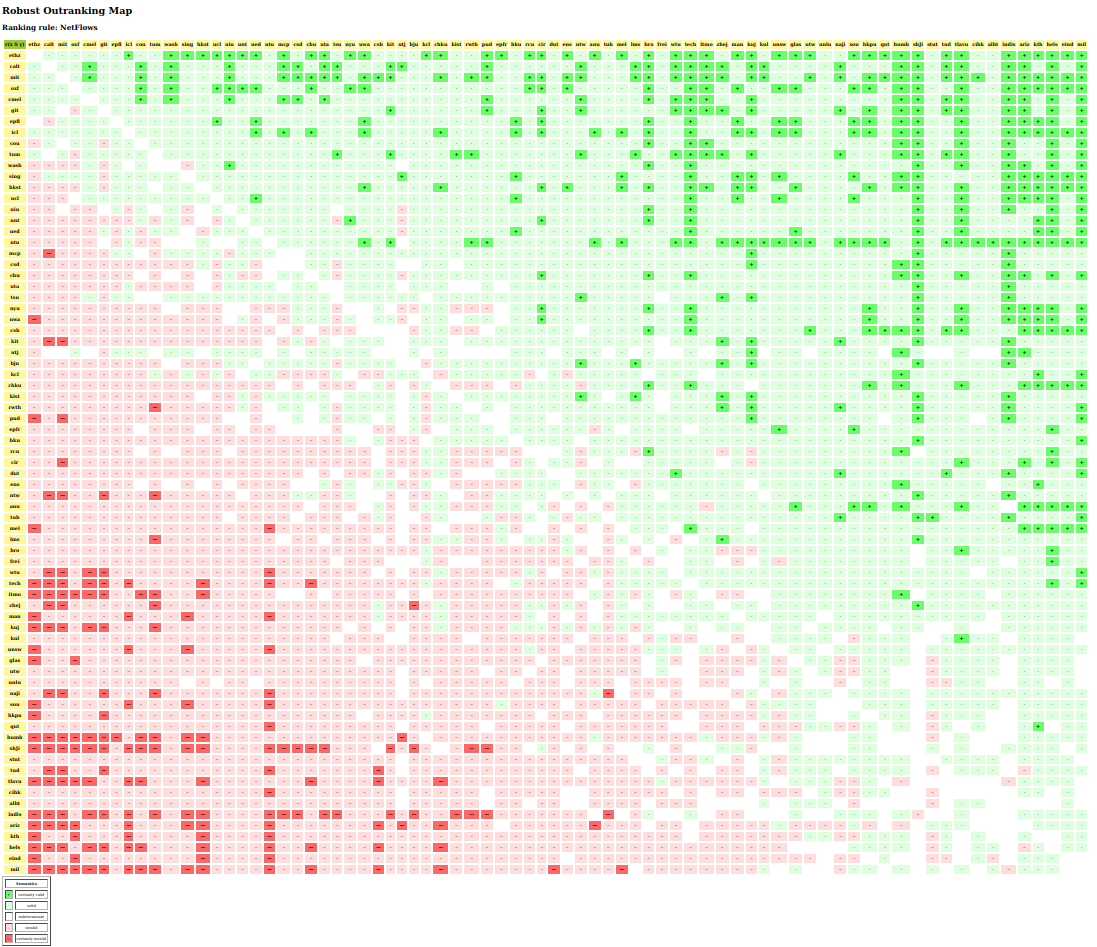
\includegraphics[width=\hsize]{Figures/13-2-the_cs_RelationMap.png}
\caption{Relation map of the robust outranking relation}
\label{fig:13.2}       % Give a unique label
\end{figure}

In Figure~\vref{fig:13.2}, \emph{dark green}, resp. \emph{light green} marked positions show certainly, resp. positively valid outranking situations, whereas \emph{dark red}, resp. \emph{light red} marked positions show certainly, respectively positively valid outranked situations. In the left upper corner one may verify that the five top-ranked Depts ([\texttt{ethz}, \texttt{calt}, \texttt{oxf}, \texttt{mit}, \texttt{cmel}]) are in fact mutually outranking each other and thus are all indifferent one to another. They give even robust \Condorcet winners by robustly outranking all other Depts.

Notice by the way that no certainly valid robust outranking (dark green) and no certainly valid robust outranked situations (dark red) appear in Figure~\vref{fig:13.3} below, resp. above the principal diagonal; none of these robust preferential situations are hence violated by the robust \NetFlows ranking. The non reflexive \emph{white} positions in the relation map, like the one between the Georgia Institute of Technology and the MIT, mark outranking or outranked situations that are not robust with respect to the given significance weight preorder. They become, hence, doubtful and are set to the indeterminate characteristic value $0.0$.

By measuring the ordinal correlation with the underlying pairwise global and marginal robust outranking situations, the quality of the robust \NetFlows ranking result can be formally evaluated with the \texttt{computeRankingCorrelation()} method\index{computeRankingCorrelation@\texttt{computeRankingCorrelation()}} and the \texttt{showCorrelation()} method\index{showCorrelation@\texttt{showCorrelation()}} (see Chap.~\ref{sec:16}).
\begin{lstlisting}[caption={Measuring the quality of the \NetFlows ranking result},label=list:13.13]
>>> corrnf = rdg.computeRankingCorrelation(nfRanking)
>>> rdg.showCorrelation(corrnf)   
  Correlation indexes:
    Crisp ordinal correlation  : +0.901
    Epistemic determination    :  0.563
    Bipolar-valued equivalence : +0.507
\end{lstlisting}

Listing~\vref{list:13.13} Line 4 indicates that the \NetFlows ranking result is indeed highly  correlated ($+0.901$, in \Kendall 's tau index sense) with the pairwise global robust outranking relation. Their bipolar-valued \emph{relational equivalence} index ($+0.51$, Line 6) indicates a more than $75\%$ criteria significance support.

With the \texttt{showRankingConsensusQuality()} method,  we can also check how the \NetFlows ranking rule is actually balancing the five ranking objectives.\index{showRankingConsensusQuality@\texttt{showRankingConsensusQua\-lity()}}
\begin{lstlisting}[caption={Measuring the consensus quality of the \NetFlows ranking result},label=list:13.14]
>>> rdg.showRankingConsensusQuality(nfRanking)
  Criterion (weight): correlation
  -------------------------------
    gtch (0.300): +0.660
    gres (0.300): +0.638
    gcit (0.275): +0.370
    gint (0.075): +0.155
    gind (0.050): +0.101
   Summary:
    Weighted mean marginal correlation (a): +0.508
    Standard deviation (b)                : +0.187
    Ranking fairness (a)-(b)              : +0.321
\end{lstlisting}

The ordinal correlation indexes with the marginal performance criterion rankings are nearly respecting the given significance weights preorder: \texttt{gtch} $\approx$ \texttt{gres} $>$ \texttt{gcit} $>$ \texttt{gint} $>$ \texttt{gind} (see Lines 4-8 above). The mean marginal ordinal correlation index is quite high ($+0.51$). Coupled with a low standard deviation ($0.187$), we obtain a quite fairly balanced ranking result (Lines 10-12). 

We can furthermore inspect with the \texttt{showCriteriaCorrelationTable()} method \index{showCriteriaCorrelationTable@\texttt{showCriteriaCorrelationTable()}} the mutual correlation indexes observed between the individual criterion based marginal robust outranking relations. 
\begin{lstlisting}[caption={Showing the ordinal correlation between the marginal criterion relations},label=list:13.15]
>>> rdg.showCriteriaCorrelationTable()
    Criteria ordinal correlation index
	 |  gcit    gind    gint    gres    gtch   
    -----|------------------------------------------
    gcit | +1.00   -0.11   +0.24   +0.13   +0.17   
    gind |         +1.00   -0.18   +0.15   +0.15   
    gint |                 +1.00   +0.04   -0.00   
    gres |                         +1.00   +0.67   
    gtch |                                 +1.00   
\end{lstlisting}

Slightly contradictory ($-0.11$) appear the \emph{Citations} and \emph{Industrial income} criteria (Line 5 Column 3 in List.~\vref{list:13.15}). Due perhaps to potential confidentiality clauses, it seams perhaps not always possible to publish industrially relevant research results in highly ranked journals. However, criteria \emph{Citations} and \emph{International outlook} show a slightly positive correlation ($+0.24$, Column 4), whereas the \emph{International outlook} criterion shows no apparent correlation with both the major \emph{Teaching} and \emph{Research} criteria. The latter are however highly correlated ($+0.67$. Line 9 Column 6).

A Principal Component Analysis may well illustrate with the \texttt{export3Dplot\-OfCriteriaCorrelation()} method the previous findings \citep{CPSTAT-L2}. \index{export3DplotOfCriteriaCorrelation@\texttt{export3DplotOfCriteria\-Correlation()}}
\begin{lstlisting}
>>> rdg.export3DplotOfCriteriaCorrelation(graphType='pdf')
\end{lstlisting}
\begin{figure}[ht]
%\sidecaption
\includegraphics[width=\hsize]{Figures/13-3-3DCorrelation.pdf}
\caption{3D PCA plot of the pairwise criteria correlation table}
\label{fig:13.3}       % Give a unique label
\end{figure}

In Figure~\vref{fig:13.3}, one may notice first that more than $80\%$ of the total variance of the previous correlation table is explained by the apparent opposition between the marginal outrankings of criteria: \emph{Teaching}, \emph{Research} and \emph{Industry income} on the left side, and the marginal outrankings of criteria: \emph{Citations} and \emph{International outlook} on the right side. Notice also in the left lower corner the nearly identical positions of the marginal outrankings of the major \emph{Teaching} and \emph{Research} criteria. In the factors 2 and 3 plot, about $30\%$ of the total variance is captured by the opposition between the marginal outrankings of the \emph{Teaching} and \emph{Research} criteria and the marginal outrankings of the \emph{Industrial income} criterion. Finally, in the factors 1 and 3 plot, nearly $15\%$ of the total variance is explained by the opposition between the marginal outrankings of the \emph{International outlook} criterion and the marginal outrankings of the \emph{Citations} criterion.

It is, finally, interesting to similarly assess the ordinal correlation between the THE average scores-based ranking and the robust outranking digraph.
\begin{lstlisting}[caption={Computing the ordinal quality of the THE ranking},label=list:13.16]
>>> # theScores = [(xScore_1,x_1), (xScore_2,x_2),... ]
>>> # is sorted in decreasing order of xscores
>>> theRanking = [item[1] for item in theScores]
>>> corrthe = rdg.computeRankingCorrelation(theRanking)
>>> rdg.showCorrelation(corrthe)
    Correlation indexes:
     Crisp ordinal correlation  : +0.907
     Epistemic determination    :  0.563
     Bipolar-valued equivalence : +0.511
>>> rdg.showRankingConsensusQuality(theRanking)
    Criterion (weight): correlation
    -------------------------------
     gtch (0.300): +0.683
     gres (0.300): +0.670
     gcit (0.275): +0.319
     gint (0.075): +0.161
     gind (0.050): +0.106
    Summary:
     Weighted mean marginal correlation (a): +0.511
     Standard deviation (b)                : +0.210
     Ranking fairness (a)-(b)              : +0.302
\end{lstlisting}

The THE ranking result is similarly correlated ($+0.907$, Line 7 in List.~\ref{list:13.16}) with the pairwise global robust outranking situations. By its overall weighted scoring rule, the THE ranking naturally induces marginal criterion correlations that are compatible with the given significance weight preorder (Lines 13-17). Notice that the mean marginal correlation is of a similar value ($+0.51$, Line 19) as the robust \NetFlows ranking. Yet, its standard deviation is slightly higher, which leads to a less fairer balancing of the three major ranking criteria.

To conclude, let us emphasise, that, without any commensurability hypothesis and by taking, furthermore, into account, first, the always present more or less imprecision of any performance evaluation and, secondly, solely ordinal criteria significance weights, we may obtain here with our robust outranking approach a very similar ranking result with a slightly better preference modelling quality. A convincing heatmap view of the 25 first-ranked Institutions may eventually be generated in the default system browser with following command.
\begin{lstlisting}
>>> rdg.showHTMLPerformanceHeatmap(
...            WithActionNames=True,\
...            outrankingModel='this',\
...            rankingRule='NetFlows',\
...            ndigits=1,\
...            Correlations=True,\
...            fromIndex=0,toIndex=25)
\end{lstlisting}
\begin{figure}[ht]
%\sidecaption
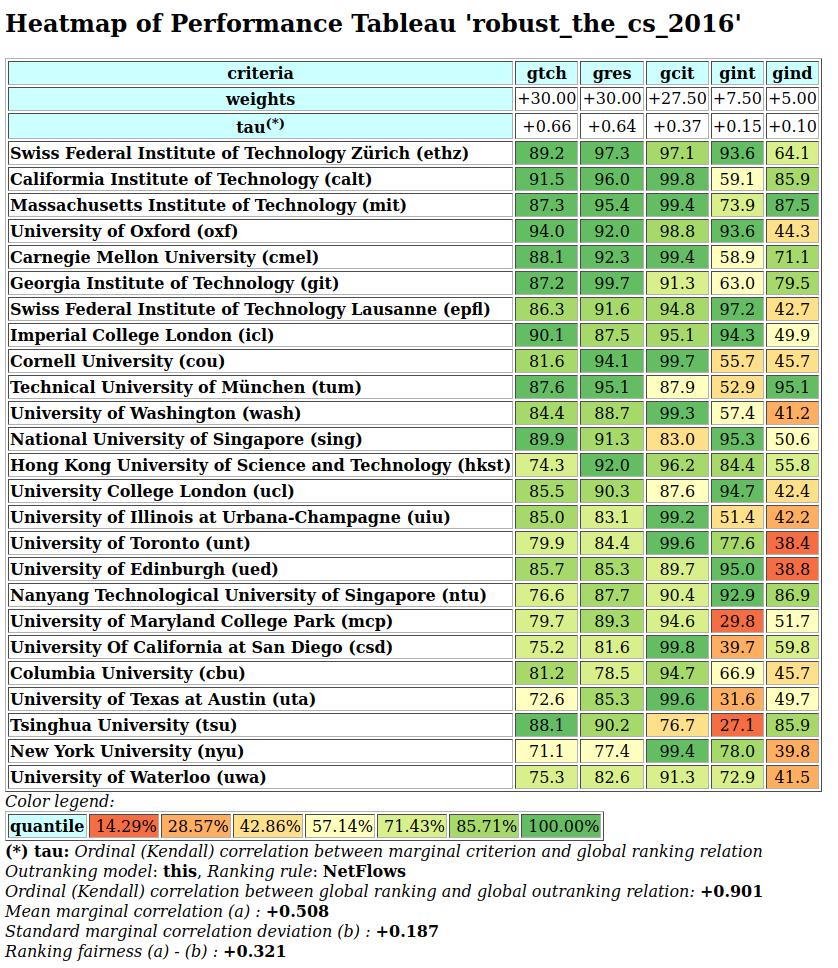
\includegraphics[width=\hsize]{Figures/13-4-theHeatmap.png}
\caption{Extract of a heatmap browser view on the \NetFlows ranking result}
\label{fig:13.4}       % Give a unique label
\end{figure}

As an exercise, the reader is invited to try out other robust outranking based ranking heuristics. Notice also that we have not challenged in this case study the THE provided criteria significance preorder. It would be very interesting to consider the five ranking objectives as equally important and, consequently, consider the ranking criteria to be equisignificant. Curious to see the ranking results under such settings.
 
%%%%%%% The chapter bibliography
%\normallatexbib
%\clearpage
\phantomsection
\addcontentsline{toc}{section}{Chapter Bibliography}
\input{02-mainMatters/13-chapterBestCSDpts.bbl}
%\bibliographystyle{spbasic}
%\bibliography{03-backMatters/reference}

%\bibliographystyle{spbasic}
%\bibliography{03-backMatters/reference}

%\bibliographystyle{spbasic}
%\bibliography{03-backMatters/reference}
